\documentclass[12pt,a4paper]{article}

\usepackage[utf8]{inputenc}
\usepackage[T1]{fontenc}
\usepackage[brazilian]{babel}
\usepackage{amsmath,amssymb}
\usepackage{graphicx}
\usepackage{float}
\usepackage{geometry}
\usepackage{setspace}
\usepackage{hyperref}
\usepackage{bookmark}
\usepackage{multirow}

% Render Unicode replacement characters as plain ASCII question marks.
\DeclareUnicodeCharacter{FFFD}{?}

\usepackage{xcolor}
\usepackage{listings}

\usepackage[nointegrals]{wasysym}

\definecolor{codegreen}{RGB}{0,120,0}
\definecolor{codegray}{RGB}{100,100,100}
\definecolor{codepurple}{RGB}{120,0,120}
\definecolor{backcolour}{RGB}{248,248,248}

% Cores do VS Code Dark+
\definecolor{vscodebackground}{HTML}{1E1E1E}
\definecolor{vscodeforeground}{HTML}{D4D4D4}
\definecolor{vscodeblue}{HTML}{569CD6}
\definecolor{vscodegreen}{HTML}{6A9955}
\definecolor{vscodeorange}{HTML}{CE9178}
\definecolor{vscodelightgreen}{HTML}{B5CEA8}
\definecolor{vscodegray}{HTML}{858585}
\definecolor{vscodecyan}{HTML}{4EC9B0}
\definecolor{vscodeyellow}{HTML}{DCDCAA}

\lstdefinestyle{fortranstyle}{
    language=[90]Fortran,
    backgroundcolor=\color{vscodebackground},
    basicstyle=\ttfamily\small\color{vscodeforeground},
    keywordstyle=\color{vscodeblue},
    commentstyle=\color{vscodegreen},
    stringstyle=\color{vscodeorange},
    numbers=left,
    numberstyle=\tiny\color{vscodegray},
    numbersep=8pt,
    frame=single,
    rulecolor=\color{vscodegray},
    breaklines=true,
    breakatwhitespace=false,
    tabsize=6,
    showstringspaces=false,
    captionpos=b,
    columns=fullflexible,
    keepspaces=true
}

\lstset{
    literate=
        {á}{{\'a}}1
        {à}{{\`a}}1
        {ã}{{\~a}}1
        {â}{{\^a}}1
        {é}{{\'e}}1
        {ê}{{\^e}}1
        {í}{{\'i}}1
        {ó}{{\'o}}1
        {ô}{{\^o}}1
        {õ}{{\~o}}1
        {ú}{{\'u}}1
        {ç}{{\c{c}}}1
        {Á}{{\'A}}1
        {À}{{\`A}}1
        {Ã}{{\~A}}1
        {Â}{{\^A}}1
        {É}{{\'E}}1
        {Ê}{{\^E}}1
        {Í}{{\'I}}1
        {Ó}{{\'O}}1
        {Ô}{{\^O}}1
        {Õ}{{\~O}}1
        {Ú}{{\'U}}1
        {Ç}{{\c{C}}}1
        {ρ}{{\ensuremath{\rho}}}1
        {τ}{{\ensuremath{\tau}}}1
        {♁}{{\ensuremath{\earth}}}1
        {–}{{\textendash}}1
}

% Margens conforme ABNT
\geometry{
    a4paper,
    left=3cm,
    right=2cm,
    top=3cm,
    bottom=2cm
}

\begin{document}

% =========================================================
% CAPA
% =========================================================

\begin{titlepage}

\begin{center}

% Instituição
{\large
UNIVERSIDADE DE SÃO PAULO
}

\vspace{0.3cm}

{\large
INSTITUTO DE FÍSICA DE SÃO CARLOS
}

\vspace{0.3cm}

{\large
BACHARELADO EM FÍSICA
}

\vfill

% Autor
{\large
CAIRO HENRIQUE VAZ COTRIM
}

\vspace{0.3cm}

{\large
No USP: 16814178
}

\vfill

% Título
{\large\bfseries
PROJETO 5 -- LEIS DE KEPLER E O PROBLEMA DE TRÊS CORPOS
}

\vspace{0.5cm}

{\normalsize
7600017 -- INTRODUÇÃO À FÍSICA COMPUTACIONAL
}

\vfill

% Local e ano
{\large
SÃO CARLOS -- SP
}

\vspace{0.3cm}

{\large
2026
}

\end{center}

\end{titlepage}


% =========================================================
% SUMÁRIO
% =========================================================

\tableofcontents
\newpage


% =========================================================
% INÍCIO DO RELATÓRIO
% =========================================================

\section*{Introdução}

O presente relatório apresenta o desenvolvimento do Projeto 5 da disciplina de Introdução à Física Computacional, cujo objetivo é estudar numericamente (com números reais de precisão dupla) o movimento de corpos sob a ação de forças centrais, com ênfase na interação gravitacional e nas leis de Kepler. São investigados problemas com diferentes configurações de sistemas gravitacionais. Os programas foram implementados em FORTRAN-77, o compilador GFortran.

\vspace{0.5cm}
\hrule
\vspace{0.5cm}

\section{Problema 1: Órbitas circulares -- comparação entre os métodos de Euler-Cromer e Verlet}

\subsection{Item (a): Determinação da velocidade inicial para órbitas circulares}

\subsubsection{Descrição do Problema}

Considera-se um planeta submetido exclusivamente à atração gravitacional do Sol, suposto fixo na origem do sistema de coordenadas. A posição inicial do planeta é dada por $\vec{\rho}_0=(a,0)$, em que $a$ corresponde ao semieixo maior da órbita, conforme os valores apresentados na Tabela I do enunciado.

O objetivo é determinar a velocidade inicial necessária para que o planeta descreva uma órbita circular. Adicionalmente, propõe-se, como desafio opcional, determinar a velocidade inicial necessária para produzir uma órbita elíptica com a excentricidade indicada na tabela.

\subsubsection{Resultados Obtidos}

Para determinar a velocidade inicial necessária à obtenção de uma órbita
elíptica de excentricidade $e$, utilizamos as relações da mecânica orbital.
A energia mecânica específica do planeta é dada por

\begin{equation}
    \varepsilon = \frac{v^2}{2} - \frac{GM_{\odot}}{r},
\end{equation}

enquanto o momento angular específico é

\begin{equation}
    h = |\vec{\rho} \times \vec{v}|.
\end{equation}

Para uma órbita elíptica, a energia mecânica específica e o momento angular
específico relacionam-se ao semieixo maior $a$ e à excentricidade $e$ por

\begin{equation}
    \varepsilon = -\frac{GM_{\odot}}{2a}
\end{equation}

e

\begin{equation}
    h^2 = GM_{\odot}a(1-e^2).
\end{equation}

Como a posição inicial é $\vec{\rho}_0=(a,0)$, temos $r_0=a$.
Além disso, escrevendo a velocidade inicial como
$\vec{v}_0=(v_{x,0},v_{y,0})$, obtemos

\begin{equation}
    h = a|v_{y,0}|.
\end{equation}

Substituindo essa expressão na relação do momento angular, resulta

\begin{equation}
    a^2v_{y,0}^2 = GM_{\odot}a(1-e^2),
\end{equation}

de onde segue que

\begin{equation}
    v_{y,0} = \sqrt{\frac{GM_{\odot}(1-e^2)}{a}},
\end{equation}

considerando o sentido positivo do eixo $y$ para a velocidade inicial.

Por sua vez, substituindo $r_0=a$ e
$v_0^2=v_{x,0}^2+v_{y,0}^2$ na expressão da energia mecânica,
temos

\begin{equation}
    \frac{v_{x,0}^2+v_{y,0}^2}{2}
    -\frac{GM_{\odot}}{a}
    =-\frac{GM_{\odot}}{2a}.
\end{equation}

Simplificando,

\begin{equation}
    v_{x,0}^2+v_{y,0}^2
    =\frac{GM_{\odot}}{a}.
\end{equation}

Utilizando o resultado obtido para $v_{y,0}$,

\begin{equation}
    v_{x,0}^2
    =\frac{GM_{\odot}}{a}
    -\frac{GM_{\odot}(1-e^2)}{a}
    =\frac{GM_{\odot}e^2}{a}.
\end{equation}

Portanto,

\begin{equation}
    v_{x,0}=-e\sqrt{\frac{GM_{\odot}}{a}},
\end{equation}

adotando o sinal negativo para que a velocidade radial inicial seja
dirigida para o Sol, conforme a configuração orbital considerada.

Nas unidades normalizadas utilizadas na simulação, em que
$GM_{\odot}=1$, as expressões finais são

\begin{equation}
    \boxed{v_{x,0}=-\frac{e}{\sqrt{a}}}
\end{equation}

\begin{equation}
    \boxed{v_{y,0}=\sqrt{\frac{1-e^2}{a}}}.
\end{equation}

\paragraph{Caso particular: órbita circular ($e=0$)}

Para uma órbita circular, a excentricidade é nula. Substituindo
$e=0$ nas expressões anteriores, obtemos

\begin{equation}
    v_{x,0}=0
\end{equation}

e

\begin{equation}
    v_{y,0}=\frac{1}{\sqrt{a}}.
\end{equation}

Assim, a velocidade inicial é exclusivamente tangencial à trajetória,
com módulo

\begin{equation}
    \boxed{v_0=\frac{1}{\sqrt{a}}}.
\end{equation}

Esse resultado corresponde à velocidade para a qual
a força gravitacional fornece exatamente a força centrípeta do movimento circular uniforme.

\subsection{Item (b): Implementação dos métodos de Euler-Cromer e Verlet}

\subsubsection{Descrição do Problema}

Neste item, deve-se desenvolver um programa em FORTRAN que calcule numericamente a posição $\vec{\rho}(\tau)$ e a velocidade $\vec{\upsilon}(\tau)$ de um planeta em função do tempo, considerando a interação gravitacional com o Sol fixo na origem.

A implementação deve contemplar dois métodos de integração numérica: Euler-Cromer, utilizando as equações discretizadas fornecidas no enunciado, e Verlet, cujas equações devem ser construídas nas unidades adimensionais adotadas. Ambos os métodos devem permitir acompanhar a evolução temporal da órbita planetária.

% ORIENTAÇÕES À IA — ESTRATÉGIA DE SOLUÇÃO
% Leia o código F77 e descreva separadamente a implementação de Euler-Cromer e a de Verlet para o movimento sob a força gravitacional do Sol fixo.
% Apresente as equações discretizadas realmente utilizadas, definindo posição, velocidade, aceleração, passo temporal e tempo adimensional. Explique a ordem de atualização das variáveis em cada método, pois ela distingue os algoritmos.
% Identifique como a aceleração gravitacional é calculada a partir da posição, como são estabelecidas as condições iniciais e como o laço temporal é organizado. Informe o intervalo de integração, o passo e os arquivos/colunas de saída conforme o código.
% Não atribua ao método de Verlet uma fórmula de velocidade ou uma variante que não esteja implementada. Se o código reconstruir a velocidade por diferença finita, explicite esse procedimento.
\subsubsection{Estratégia de Solução}

O movimento do planeta é descrito nas unidades adimensionais
adotadas no enunciado, nas quais a aceleração gravitacional é
dada por

\begin{equation}
    \vec{a}(\tau) =
    -\frac{\vec{\rho}(\tau)}{\rho(\tau)^3},
\end{equation}

em que $\vec{\rho}=(\rho_x,\rho_y)$ representa a posição
adimensional do planeta, $\rho=|\vec{\rho}|$ é sua distância
ao Sol e $\tau$ é o tempo adimensional. Definindo
$\Delta\tau$ como o passo temporal, os dois métodos são
implementados iterativamente a partir das mesmas condições
iniciais.

\paragraph{Método de Euler-Cromer}

No método de Euler-Cromer, a velocidade é atualizada
primeiramente, utilizando a aceleração calculada a partir
da posição no instante atual. Em seguida, a posição é
atualizada utilizando a nova velocidade. Assim, as equações
discretizadas implementadas são

\begin{equation}
    \vec{\upsilon}_{i+1}
    =
    \vec{\upsilon}_i
    -
    \frac{\vec{\rho}_i}{\rho_i^3}\Delta\tau,
\end{equation}

\begin{equation}
    \vec{\rho}_{i+1}
    =
    \vec{\rho}_i
    +
    \vec{\upsilon}_{i+1}\Delta\tau.
\end{equation}

A distância $\rho_i$ é calculada a partir das componentes
da posição no instante atual:

\begin{equation}
    \rho_i =
    \sqrt{\rho_{x,i}^2+\rho_{y,i}^2}.
\end{equation}

No código, as atualizações são realizadas separadamente
para as componentes $x$ e $y$, mantendo a mesma ordem:
primeiro a velocidade e depois a posição. A cada iteração,
o estado do planeta é registrado no arquivo
\texttt{tarefa-1b-saida-1.dat}, contendo, respectivamente,
o tempo adimensional, as posições $\rho_x$ e $\rho_y$ e
as velocidades $\upsilon_x$ e $\upsilon_y$.

\paragraph{Método de Verlet}

Para o método de Verlet, utiliza-se uma equação de
recorrência para calcular diretamente as posições a partir
das posições nos dois instantes anteriores. Como essa
formulação necessita de duas posições iniciais, a segunda
posição é inicialmente estimada por

\begin{equation}
    \vec{\rho}_2 =
    \vec{\rho}_1 +
    \vec{\upsilon}_1\Delta\tau.
\end{equation}

Essa estimativa corresponde à utilização de uma aproximação
de primeira ordem, sem a inclusão do termo de aceleração
na inicialização.

A partir do segundo passo, as posições são atualizadas
pela equação de Verlet:

\begin{equation}
    \vec{\rho}_{i+1}
    =
    2\vec{\rho}_i-\vec{\rho}_{i-1}
    -
    \frac{\vec{\rho}_i}{\rho_i^3}
    \Delta\tau^2.
\end{equation}

Assim como no método anterior, a distância $\rho_i$ é
calculada a partir das componentes da posição atual.
Após a determinação da nova posição, as velocidades são
reconstruídas por meio de diferenças finitas centradas:

\begin{equation}
    \vec{\upsilon}_i =
    \frac{\vec{\rho}_{i+1}-\vec{\rho}_{i-1}}
    {2\Delta\tau}.
\end{equation}

Portanto, diferentemente do método de Euler-Cromer,
a velocidade não é atualizada diretamente por uma
equação de evolução independente, mas estimada a partir
das posições nos instantes anterior e posterior ao
instante considerado.

Os resultados são armazenados no arquivo
\texttt{tarefa-1b-saida-2.dat}, seguindo a mesma organização
de colunas utilizada na saída do método de Euler-Cromer.

\paragraph{Condições iniciais e parâmetros de integração}

Para a simulação apresentada, foram utilizadas as
condições iniciais correspondentes a uma órbita circular,
com semieixo maior $a=1$ e excentricidade $e=0$.
Consequentemente,

\begin{equation}
    \vec{\rho}_0=(1,0),
    \qquad
    \vec{\upsilon}_0=(0,1).
\end{equation}

O período orbital adimensional é determinado pela
terceira lei de Kepler,

\begin{equation}
    T=2\pi a^{3/2}=2\pi.
\end{equation}

A integração é realizada durante dez períodos orbitais,
de modo que o tempo máximo é

\begin{equation}
    \tau_{\max}=10T=20\pi.
\end{equation}

Adotou-se o passo temporal constante
$\Delta\tau=0,01$, resultando em

\begin{equation}
    N=\operatorname{int}\left(
    \frac{\tau_{\max}}{\Delta\tau}
    \right)=6283
\end{equation}

iterações. Os dois métodos utilizam, portanto, as mesmas
condições iniciais, o mesmo intervalo nominal de
integração e o mesmo passo temporal, permitindo comparar
as trajetórias obtidas numericamente.

\begin{lstlisting}[
style=fortranstyle
]
      program tarefa1b
      ! Órbitas circulares: comparação entre os métodos de EC e Verlet.
      ! Utiliza-se a 3a Lei de Kepler GM = 4pi^2 UA^3 ano^(-2).
      ! Grandezas adimensionais rho = r/UA, tau = 2pi*t/ano, v = v/(2pi*UA/ano).
      ! Toma-se o Sol como origem estática e a Terra como corpo em órbita.

      implicit none

      integer*4 i, nsteps
      real*8 a, e, tau, periodo, taumax, dtau
      real*8 rx(10000), ry(10000), vx(10000), vy(10000), r(10000)
      real*8 pi
      parameter (pi = 3.14159265358979323d0)

      ! Condições iniciais adimensionais
      a = 1.0d0 ! semieixo maior da órbita elíptica
      e = 0.0d0 ! excentricidade da órbita elíptica
      rx(1) = a ! posição inicial no eixo x
      ry(1) = 0.0d0 ! posição inicial no eixo y
      vx(1) = - e / sqrt(a) ! velocidade inicial no eixo x
      vy(1) = sqrt((1.0d0-e**2)/a) ! velocidade inicial no eixo y para a órbita elíptica especificada acima

      ! Parâmetros da simulação
      periodo = 2.0d0 * pi * a**(3d0/2d0) ! período adimensional (3a Lei de Kepler)
      taumax = 10.0d0 * periodo ! 10 períodos adimensionais
      dtau = 0.01d0 ! passo de tempo adimensional

      ! Número de passos da simulação
      nsteps = int(taumax/dtau)

      ! Simulação via método de Euler-Cromer
      open(10, file='tarefa-1b-saida-1.dat')

      do i = 1, nsteps

        tau = (i-1)*dtau
        write(10,*) tau, rx(i), ry(i), vx(i), vy(i)

        ! Atualização da distância
        r(i) = sqrt(rx(i)**2 + ry(i)**2)

        ! Atualização das posições e velocidades
        vx(i+1) = vx(i) - (rx(i)/r(i)**3)*dtau
        rx(i+1) = rx(i) + vx(i+1)*dtau
        vy(i+1) = vy(i) - (ry(i)/r(i)**3)*dtau
        ry(i+1) = ry(i) + vy(i+1)*dtau

      end do

      close(10)

      ! Simulação via método de Verlet
      ! Para o método de Verlet, precisamos de uma segunda posição inicial
      ! Calculamos os valores de rx(1), ry(1), vx(1), vy(1)
      ! por meio do método de Euler para calcular a posição do passo i=2
      open(20, file='tarefa-1b-saida-2.dat')

      write(20,*) 0.0d0, rx(1), ry(1), vx(1), vy(1)

      rx(2) = rx(1) + vx(1)*dtau
      ry(2) = ry(1) + vy(1)*dtau

      do i = 2, nsteps

        ! Atualização da distância
        r(i) = sqrt(rx(i)**2 + ry(i)**2)

        ! Atualização das posições
        rx(i+1) = 2.0d0*rx(i) - rx(i-1) - (rx(i)/r(i)**3)*dtau**2
        ry(i+1) = 2.0d0*ry(i) - ry(i-1) - (ry(i)/r(i)**3)*dtau**2

        ! Atualização das velocidades
        vx(i) = (rx(i+1) - rx(i-1))/(2.0d0*dtau)
        vy(i) = (ry(i+1) - ry(i-1))/(2.0d0*dtau)

        tau = (i-1)*dtau
        write(20,*) tau, rx(i), ry(i), vx(i), vy(i)

      end do

      close(20)

      end program
\end{lstlisting}


% ORIENTAÇÕES À IA — RESULTADOS OBTIDOS
% Descreva as trajetórias geradas por cada método e faça referência aos gráficos efetivamente fornecidos, identificando método, condições iniciais e parâmetros relevantes.
% Compare quantitativamente as órbitas: circularidade, raio orbital, período, precessão ou deriva, conforme seja possível avaliar nos dados. Não afirme que as trajetórias coincidem ou diferem sem evidência.
% Relacione as diferenças observadas às propriedades numéricas dos métodos, distinguindo comportamento efetivamente observado de expectativas teóricas.
\subsubsection{Resultados Obtidos}

\subsubsection{Resultados Obtidos}

As Figuras \ref{fig:orbita-euler-cromer} e
\ref{fig:orbita-verlet} apresentam as trajetórias
planetárias obtidas pelos métodos de Euler-Cromer e
Verlet, respectivamente, para as condições iniciais
$a=1$ e $e=0$, com passo temporal $\Delta\tau=0,01$.
Em ambos os casos, a integração foi realizada durante
dez períodos orbitais, com tempo máximo nominal
$\tau_{\max}=20\pi$.

\begin{figure}[htbp]
    \centering
    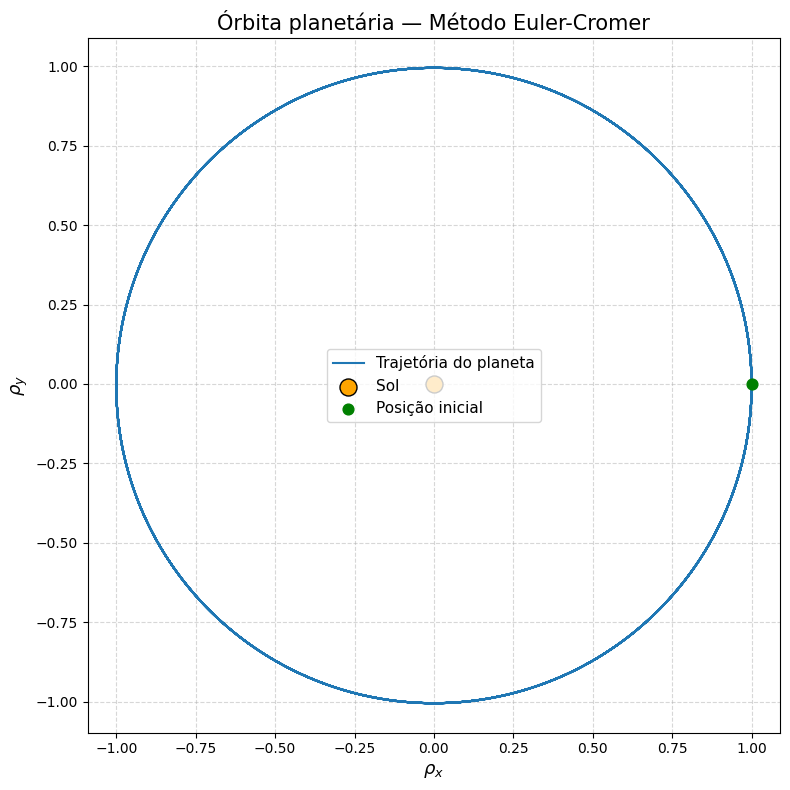
\includegraphics[width=0.75\textwidth]
    {tarefa-1b-grafico-1.png}
    \caption{Trajetória planetária obtida pelo método
    de Euler-Cromer para uma órbita circular.}
    \label{fig:orbita-euler-cromer}
\end{figure}

\begin{figure}[htbp]
    \centering
    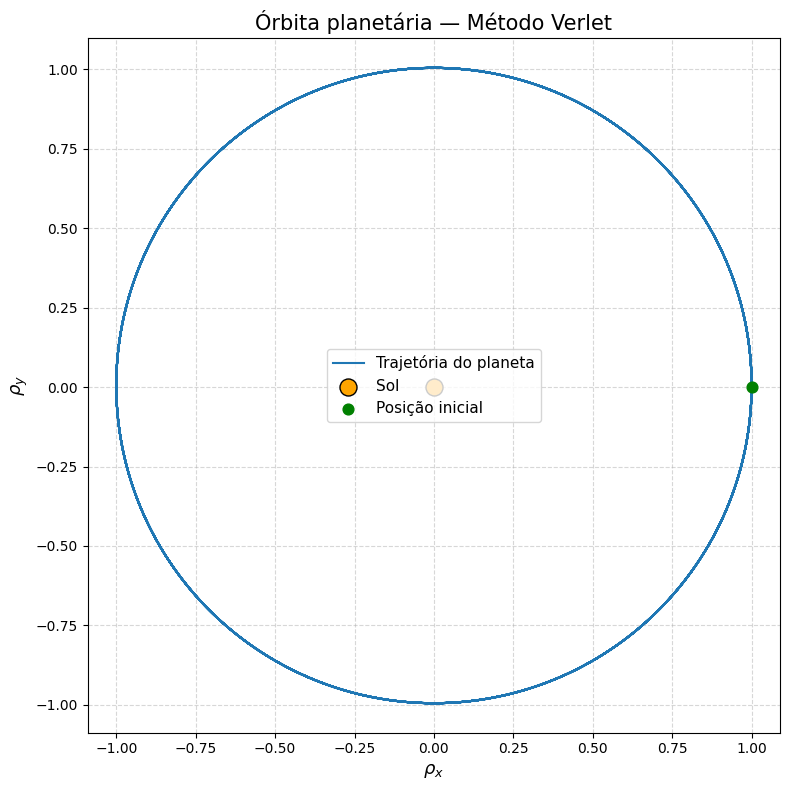
\includegraphics[width=0.75\textwidth]
    {tarefa-1b-grafico-2.png}
    \caption{Trajetória planetária obtida pelo método
    de Verlet para uma órbita circular.}
    \label{fig:orbita-verlet}
\end{figure}

No caso do método de Euler-Cromer, observa-se uma
trajetória aproximadamente circular, centrada na origem
do sistema de coordenadas, onde se encontra o Sol.
O planeta parte da posição inicial
$\vec{\rho}_0=(1,0)$ e percorre uma órbita cujo raio
permanece visualmente próximo de uma unidade ao longo
da simulação.

De maneira análoga, a trajetória obtida pelo método
de Verlet também apresenta formato aproximadamente
circular, com centro na origem e raio orbital próximo
de uma unidade. A posição inicial do planeta coincide
com aquela utilizada na simulação anterior, permitindo
uma comparação direta entre os resultados dos dois
algoritmos.

Comparando as duas figuras, não se observa diferença
visual significativa entre as trajetórias produzidas
pelos métodos de Euler-Cromer e Verlet. Ambas
representam órbitas aproximadamente circulares,
sem evidências visuais de deriva radial ou precessão
apreciável na escala apresentada. Portanto, para as
condições iniciais e o passo temporal adotados,
os dois métodos reproduzem qualitativamente o
movimento circular esperado.

\subsection{Item (c): Estabilidade das órbitas e determinação do passo temporal máximo}

\subsubsection{Descrição do Problema}

Neste item, deve-se investigar a estabilidade numérica das órbitas circulares ao longo de muitas revoluções, para os métodos de Euler-Cromer e Verlet. Para isso, define-se a grandeza

\begin{equation}
    \delta = \frac{\rho_{\max}}{\rho_{\min}}-1,
\end{equation}

em que $\rho_{\max}$ e $\rho_{\min}$ representam, respectivamente, as distâncias máxima e mínima entre o planeta e o Sol durante a simulação.

O objetivo é construir gráficos de $\delta$ em função do passo temporal $\Delta\tau$ e determinar o maior passo temporal $\Delta\tau_{\max}$ para o qual $\delta<10^{-3}$, considerando também todos os passos menores. Deve-se investigar a dependência de $\Delta\tau_{\max}$ com o semieixo maior $a$, verificando se $\Delta\tau_{\max}\propto a^{3/2}$ para ambos os métodos, e relacionar esse comportamento à terceira lei de Kepler.

% ORIENTAÇÕES À IA — ESTRATÉGIA DE SOLUÇÃO
% Examine o código F77 responsável pela varredura de passos temporais e explique como são gerados os valores de Δτ testados para cada semieixo maior e para cada integrador.
% Descreva como o programa acompanha a distância planetária ρ, determina ρ_max e ρ_min e calcula δ = ρ_max/ρ_min - 1. Especifique o número de revoluções ou o intervalo simulado e os critérios usados para selecionar Δτ_max.
% Explique como é garantida a condição do enunciado de que δ < 10-³ também para todos os passos menores, conforme a lógica efetivamente implementada. Descreva a busca pelo limite, as funções auxiliares e eventuais critérios de refinamento presentes no código.
% Explique como Δτ_max é obtido para diferentes valores de a e como é feita a análise de proporcionalidade com a^(3/2), por exemplo, por normalização ou ajuste em escala logarítmica, somente se isso constar no procedimento.
\subsubsection{Estratégia de Solução}

\paragraph{Cálculo de $\delta$}

Foram implementadas duas funções auxiliares,
\texttt{get\_delta\_euler\_cromer} e
\texttt{get\_delta\_verlet}, responsáveis por simular
o movimento planetário com cada integrador e calcular
a grandeza $\delta$.

Em ambas as funções, as condições iniciais são
reinicializadas a cada avaliação. Considerando
a excentricidade $e=0$, a posição e a velocidade
iniciais são dadas por

\begin{equation}
    \vec{\rho}_0=(a,0),
    \qquad
    \vec{\upsilon}_0=
    \left(0,\frac{1}{\sqrt{a}}\right).
\end{equation}

O número de passos de integração é determinado por

\begin{equation}
    N=\operatorname{nint}\left(
    \frac{\tau_{\max}}{\Delta\tau}
    \right),
\end{equation}

em que $\operatorname{nint}$ representa o arredondamento
para o inteiro mais próximo.

No método de Euler-Cromer, a cada iteração são atualizadas
primeiramente as componentes da velocidade e, em seguida,
as componentes da posição, utilizando a aceleração
gravitacional calculada a partir da posição atual.
Após cada atualização, calcula-se a distância

\begin{equation}
    \rho_i=\sqrt{x_i^2+y_i^2},
\end{equation}

que é utilizada para atualizar os extremos por meio
das funções intrínsecas \texttt{min} e \texttt{max}
do FORTRAN.

No método de Verlet, são inicialmente calculadas
duas posições: a posição inicial e uma segunda posição
estimada pelo método de Euler, conforme

\begin{equation}
    \vec{\rho}_1=
    \vec{\rho}_0+\vec{\upsilon}_0\Delta\tau.
\end{equation}

Em seguida, as posições são atualizadas pela relação

\begin{equation}
    \vec{\rho}_{i+1}
    =
    2\vec{\rho}_i-\vec{\rho}_{i-1}
    -
    \frac{\vec{\rho}_i}{\rho_i^3}\Delta\tau^2.
\end{equation}

A cada atualização, a distância ao Sol também é
calculada e utilizada para determinar os valores
máximo e mínimo. Ao término da integração, ambas
as funções retornam

\begin{equation}
    \delta=\frac{\rho_{\max}}{\rho_{\min}}-1.
\end{equation}

\paragraph{Variação do passo temporal}

Primeiramente, investigou-se a dependência de $\delta$
com o passo temporal para o caso particular $a=1$.
O programa realiza dez avaliações, utilizando passos
temporais da forma

\begin{equation}
    \Delta\tau=10^{-i},
    \qquad i=1,2,\ldots,10.
\end{equation}

Para cada valor de $\Delta\tau$, são calculados
separadamente os valores de $\delta$ pelos métodos
de Euler-Cromer e Verlet. Os resultados são armazenados,
respectivamente, nos arquivos
\texttt{tarefa-1c-saida-1.dat} e
\texttt{tarefa-1c-saida-2.dat}.

Em todas essas simulações, o intervalo de integração
corresponde a dez períodos orbitais. Conforme a
terceira lei de Kepler nas unidades adimensionais
adotadas, o período é

\begin{equation}
    T=2\pi a^{3/2},
\end{equation}

de modo que o tempo máximo de integração é

\begin{equation}
    \tau_{\max}=10T=20\pi a^{3/2}.
\end{equation}

\paragraph{Determinação de $\Delta\tau_{\max}$}

Para determinar o maior passo temporal que satisfaz
o critério de estabilidade, foram implementadas
as funções \texttt{get\_dtau\_max\_euler\_cromer}
e \texttt{get\_dtau\_max\_verlet}. Ambas utilizam
o mesmo procedimento de busca, diferenciando-se
apenas pela função de cálculo de $\delta$ empregada.

Inicialmente, estabelece-se um limite superior
$\Delta\tau_{\mathrm{sup}}=10^{-1}$, que é testado
diretamente. Caso satisfaça $\delta<10^{-3}$,
esse valor é retornado. Caso contrário, inicia-se
uma busca progressiva, na qual o limite superior
é sucessivamente dividido por dois. O limite
inferior é definido como

\begin{equation}
    \Delta\tau_{\mathrm{inf}}
    =\frac{\Delta\tau_{\mathrm{sup}}}{2},
\end{equation}

com valor mínimo imposto de $10^{-6}$.

Esse procedimento é repetido até encontrar um passo
que satisfaça o critério de estabilidade ou atingir
o limite mínimo estabelecido no código. Quando
é encontrado um intervalo cujos extremos apresentam
resultados distintos em relação ao critério, realiza-se
um refinamento por busca binária, com vinte iterações.

Em cada iteração do refinamento, calcula-se o ponto
médio do intervalo:

\begin{equation}
    \Delta\tau=
    \frac{\Delta\tau_{\mathrm{inf}}+
    \Delta\tau_{\mathrm{sup}}}{2}.
\end{equation}

Se o valor calculado de $\delta$ for inferior a
$10^{-3}$, atualiza-se o limite inferior. Caso
contrário, atualiza-se o limite superior. Ao final,
a função retorna o limite inferior, correspondente
ao maior passo encontrado dentro da precisão
proporcionada pelo refinamento.

\paragraph{Dependência com o semieixo maior}

Por fim, investiga-se a dependência do passo temporal
máximo com o semieixo maior da órbita. Para isso,
são considerados cem valores de $a$, igualmente
espaçados no intervalo

\begin{equation}
    0,1\leq a\leq 2,0,
\end{equation}

com incremento

\begin{equation}
    \Delta a=\frac{2,0-0,1}{99}.
\end{equation}

Para cada valor de $a$, o período orbital e o tempo
máximo de integração são recalculados. Em seguida,
determina-se $\Delta\tau_{\max}$ separadamente
para os métodos de Euler-Cromer e Verlet, utilizando
as respectivas funções de busca.

Os pares $(a,\Delta\tau_{\max})$ são armazenados
nos arquivos \texttt{tarefa-1c-saida-3.dat} e
\texttt{tarefa-1c-saida-4.dat}, permitindo construir
os gráficos da dependência do passo temporal máximo
com o semieixo maior para os dois integradores.

\begin{lstlisting}[
style=fortranstyle
]
      program tarefa1c
      ! Órbitas circulares: escolhendo dtau para que a órbita seja estável nos métodos de Euler-Cromer e Verlet
      ! e verificando a 3a Lei de Kepler.
      ! Utiliza-se a 3a Lei de Kepler GM = 4pi^2 UA^3 ano^(-2).
      ! Grandezas adimensionais rho = r/UA, tau = 2pi*t/ano, v = v/(2pi*UA/ano).
      ! Toma-se o Sol como origem estática e a Terra como corpo em órbita.

      implicit none

      integer*4 i

      real*8 a, e, periodo, taumax
      real*8 dtau
      real*8 dtau_ec, dtau_v
      real*8 amin, amax, da
      integer*4 num_a

      real*8 get_delta_euler_cromer, get_delta_verlet
      real*8 get_dtau_max_euler_cromer, get_dtau_max_verlet

      real*8 pi
      parameter (pi = 3.14159265358979323d0)

      ! Condicoes iniciais adimensionais
      e = 0.0d0 ! excentricidade da órbita elíptica

      ! Parametros da variacao de a
      num_a = 100 ! numero de valores de a
      amin = 0.1d0 ! a mínimo
      amax = 2.0d0 ! a máximo
      da = (amax-amin)/dble(num_a-1) ! Incremento de a

      ! Arquivos de saida
      open(10, file='tarefa-1c-saida-1.dat')
      open(20, file='tarefa-1c-saida-2.dat')
      open(30, file='tarefa-1c-saida-3.dat')
      open(40, file='tarefa-1c-saida-4.dat')

      ! ! delta em função de dtau ! !
      a = 1.0d0 ! semieixo maior da órbita elíptica
      periodo = 2.0d0*pi*a**(3.0d0/2.0d0)
      taumax = 10.0d0*periodo
      do i = 1, 10

        dtau = 10.0d0**(-dble(i))

        ! Escrita dos resultados
        write(10,*) dtau, get_delta_euler_cromer(
     &     taumax, dtau, a, e)
        write(20,*) dtau, get_delta_verlet(
     &     taumax, dtau, a, e)

      end do

      close(10)
      close(20)

      ! ! dtau_max em função de a ! !
      do i = 1, num_a

        a = amin + dble(i-1)*da

        ! Parâmetros da simulação
        periodo = 2.0d0*pi*a**(3.0d0/2.0d0)
        taumax = 10.0d0*periodo

        ! Metodo de Euler-Cromer
        dtau_ec = get_dtau_max_euler_cromer(
     &       taumax, a, e)

        ! Metodo de Verlet
        dtau_v = get_dtau_max_verlet(
     &       taumax, a, e)

        ! Escrita dos resultados
        write(30,*) a, dtau_ec
        write(40,*) a, dtau_v

      end do

      close(30)
      close(40)

      end program 

      function get_delta_euler_cromer(taumax, dtau, a, e)
      ! Simulação de órbita gravitacional via método de Euler-Cromer
      ! Retorna delta = (rho_max / rho_min) - 1, para verificar a estabilidade da órbita.

        implicit none
        integer*4 i, nsteps
        real*8 taumax, dtau, a, e
        real*8 x, y, vx, vy, r, rmin, rmax
        real*8 get_delta_euler_cromer

        ! Reinicializacao das condicoes iniciais
        x = a
        y = 0.0d0
        vx = -e/sqrt(a)
        vy = sqrt((1.0d0-e**2)/a)

        nsteps = nint(taumax/dtau)

        ! Inicializacao dos extremos
        r = sqrt(x**2 + y**2)
        rmin = r
        rmax = r

        ! Integracao por Euler-Cromer
        do i = 1, nsteps

            r = sqrt(x**2 + y**2)

            ! Atualizacao das velocidades
            vx = vx - (x/r**3)*dtau
            vy = vy - (y/r**3)*dtau

            ! Atualizacao das posicoes
            x = x + vx*dtau
            y = y + vy*dtau

            ! Atualizacao dos extremos do raio
            r = sqrt(x**2 + y**2)

            rmin = min(rmin, r)
            rmax = max(rmax, r)

        end do

        get_delta_euler_cromer = (rmax/rmin) - 1.0d0

      end function


      function get_delta_verlet(taumax, dtau, a, e)
      ! Simulação de órbita gravitacional via método de Verlet
      ! Retorna delta = (rho_max / rho_min) - 1, para verificar a estabilidade da órbita.

        implicit none
        integer*4 i, nsteps
        real*8 taumax, dtau, a, e
        real*8 xprev, yprev, xcurr, ycurr
        real*8 xnext, ynext, vx0, vy0
        real*8 r, rmin, rmax
        real*8 get_delta_verlet

        ! Condicoes iniciais
        xprev = a
        yprev = 0.0d0
        vx0 = -e/sqrt(a)
        vy0 = sqrt((1.0d0-e**2)/a)

        nsteps = nint(taumax/dtau)

        ! Inicializacao dos extremos
        r = sqrt(xprev**2 + yprev**2)
        rmin = r
        rmax = r

        ! Segunda posicao calculada pelo metodo de Euler
        xcurr = xprev + vx0*dtau
        ycurr = yprev + vy0*dtau

        r = sqrt(xcurr**2 + ycurr**2)
        rmin = min(rmin, r)
        rmax = max(rmax, r)

        ! Integracao por Verlet
        do i = 2, nsteps

            r = sqrt(xcurr**2 + ycurr**2)

            ! Atualizacao das posicoes
            xnext = 2.0d0*xcurr - xprev - (xcurr/r**3)*dtau**2

            ynext = 2.0d0*ycurr - yprev - (ycurr/r**3)*dtau**2

            ! Atualizacao dos extremos do raio
            r = sqrt(xnext**2 + ynext**2)

            rmin = min(rmin, r)
            rmax = max(rmax, r)

            ! Avanco dos passos temporais
            xprev = xcurr
            yprev = ycurr

            xcurr = xnext
            ycurr = ynext

        end do

        get_delta_verlet = (rmax/rmin) - 1.0d0

      end function


      function get_dtau_max_euler_cromer(
     &     taumax, a, e)

      implicit none

      real*8 taumax, a, e
      real*8 dtau, delta
      real*8 dtau_inf, dtau_sup
      real*8 get_delta_euler_cromer
      real*8 get_dtau_max_euler_cromer

      integer i

      get_dtau_max_euler_cromer = 0.0d0

      ! Intervalo inicial
      dtau_sup = 1.0d-1

      ! Testa o maior passo inicial
      delta = get_delta_euler_cromer(
     &       taumax, dtau_sup, a, e)

      if (delta .lt. 1.0d-3) then
        get_dtau_max_euler_cromer = dtau_sup
        return
      end if

      ! Busca progressiva do intervalo
      do i = 1, 20

        dtau_inf = dtau_sup/2.0d0

        if (dtau_inf .lt. 1.0d-6) then
          dtau_inf = 1.0d-6
        end if

        delta = get_delta_euler_cromer(
     &         taumax, dtau_inf, a, e)

        if (delta .lt. 1.0d-3) exit

        dtau_sup = dtau_inf

        if (dtau_sup .le. 1.0d-6) return

      end do

      ! Refinamento por busca binaria
      do i = 1, 20

        dtau = (dtau_inf + dtau_sup)/2.0d0

        delta = get_delta_euler_cromer(
     &         taumax, dtau, a, e)

        if (delta .lt. 1.0d-3) then
          dtau_inf = dtau
        else
          dtau_sup = dtau
        end if

      end do

      get_dtau_max_euler_cromer = dtau_inf

      return
      end function


      function get_dtau_max_verlet(
     &     taumax, a, e)

      implicit none

      real*8 taumax, a, e
      real*8 dtau, delta
      real*8 dtau_inf, dtau_sup
      real*8 get_delta_verlet
      real*8 get_dtau_max_verlet

      integer i

      get_dtau_max_verlet = 0.0d0

      ! Intervalo inicial
      dtau_sup = 1.0d-1

      ! Testa o maior passo inicial
      delta = get_delta_verlet(
     &       taumax, dtau_sup, a, e)

      if (delta .lt. 1.0d-3) then
        get_dtau_max_verlet = dtau_sup
        return
      end if

      ! Busca progressiva do intervalo
      do i = 1, 20

        dtau_inf = dtau_sup/2.0d0

        if (dtau_inf .lt. 1.0d-6) then
          dtau_inf = 1.0d-6
        end if

        delta = get_delta_verlet(
     &         taumax, dtau_inf, a, e)

        if (delta .lt. 1.0d-3) exit

        dtau_sup = dtau_inf

        if (dtau_sup .le. 1.0d-6) return

      end do

      ! Refinamento por busca binaria
      do i = 1, 20

        dtau = (dtau_inf + dtau_sup)/2.0d0

        delta = get_delta_verlet(
     &         taumax, dtau, a, e)

        if (delta .lt. 1.0d-3) then
          dtau_inf = dtau
        else
          dtau_sup = dtau
        end if

      end do

      get_dtau_max_verlet = dtau_inf

      return
      end function
\end{lstlisting}


% ORIENTAÇÕES À IA — RESULTADOS OBTIDOS
% Apresente os gráficos de δ em função de Δτ para os casos calculados, distinguindo Euler-Cromer e Verlet. Descreva as regiões que satisfazem ou não o limiar de 10-³.
% Informe os valores de Δτ_max para cada a e método em tabela ou no texto, com precisão compatível com a busca numérica.
% Analise a dependência de Δτ_max com a. Compare os dados com a lei de escala a^(3/2), incluindo constante de proporcionalidade, razão normalizada ou expoente ajustado apenas quando esses valores puderem ser obtidos dos dados.
% Discuta diferenças entre os integradores e possíveis limitações da busca, sem extrapolar além dos casos simulados.
\subsubsection{Resultados Obtidos}

\subsubsection{Resultados Obtidos}

A Figura \ref{fig:estabilidade-dtau} apresenta a
dependência da grandeza $\delta$ com o passo temporal
$\Delta\tau$, para uma órbita circular com semieixo
maior $a=1$. A linha horizontal tracejada representa
o limite de estabilidade estabelecido,
$\delta=10^{-3}$.

\begin{figure}[htbp]
    \centering
    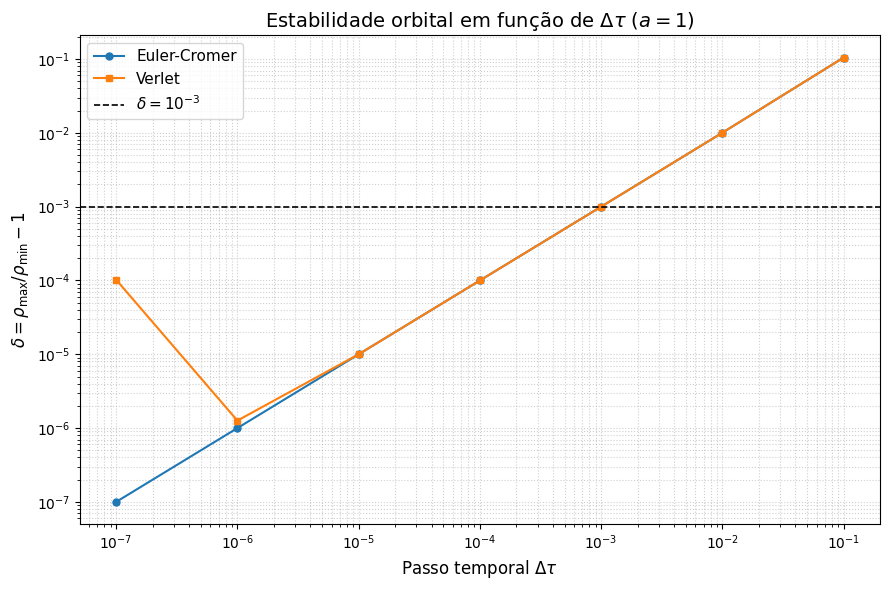
\includegraphics[width=0.9\textwidth]
    {tarefa-1c-grafico-1.png}
    \caption{Estabilidade orbital em função do passo
    temporal para os métodos de Euler-Cromer e Verlet,
    considerando $a=1$. A linha tracejada indica
    o limite $\delta=10^{-3}$.}
    \label{fig:estabilidade-dtau}
\end{figure}

Observa-se que, para ambos os métodos, a grandeza
$\delta$ apresenta uma tendência crescente com o
aumento de $\Delta\tau$. Para os passos temporais
representados no gráfico, os valores de $\delta$
permanecem abaixo do limite estabelecido quando
$\Delta\tau$ é suficientemente pequeno. À medida que
o passo aumenta, a grandeza se aproxima do limiar
e passa a ultrapassá-lo.

Para o método de Euler-Cromer, observa-se uma
relação aproximadamente crescente entre $\delta$
e $\Delta\tau$ ao longo dos pontos apresentados.
No método de Verlet, o comportamento é semelhante
para a maior parte dos passos temporais, embora
o ponto correspondente a $\Delta\tau=10^{-7}$
apresente um valor de $\delta$ aproximadamente
igual a $10^{-4}$, destoando da tendência dos
pontos vizinhos. Apesar dessa particularidade,
esse ponto também permanece abaixo do limite
de estabilidade estabelecido.

A segunda análise consiste na determinação do
passo temporal máximo para diferentes valores do
semieixo maior. Os resultados obtidos são apresentados
na Figura \ref{fig:dtau-max-a}.

\begin{figure}[htbp]
    \centering
    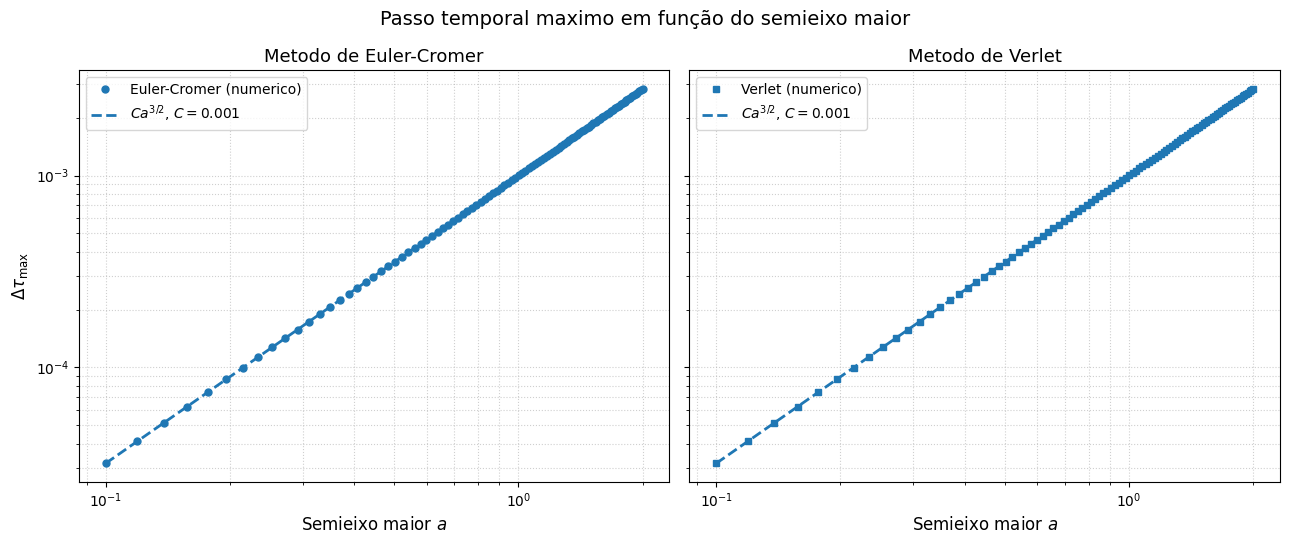
\includegraphics[width=\textwidth]
    {tarefa-1c-grafico-2.png}
    \caption{Dependência do passo temporal máximo
    com o semieixo maior para os métodos de
    Euler-Cromer e Verlet. As linhas tracejadas
    representam a relação de referência
    $\Delta\tau_{\max}=Ca^{3/2}$, com $C=0,001$.}
    \label{fig:dtau-max-a}
\end{figure}

Os resultados mostram que o passo temporal máximo
aumenta com o semieixo maior para ambos os métodos.
Além disso, os pontos numéricos apresentam boa
concordância visual com a curva de referência

\begin{equation}
    \Delta\tau_{\max}=Ca^{3/2},
\end{equation}

utilizada nos gráficos com $C=0,001$. Essa
concordância indica que, para o intervalo de
semieixos maiores investigado, a dependência
encontrada é compatível com

\begin{equation}
    \boxed{\Delta\tau_{\max}\propto a^{3/2}}.
\end{equation}

Esse comportamento pode ser relacionado diretamente
à terceira lei de Kepler, segundo a qual o período
orbital é proporcional a $a^{3/2}$. Como o tempo
de integração corresponde a dez períodos orbitais,
o tempo total simulado também aumenta com essa
mesma potência do semieixo maior. Dessa forma,
a dependência observada para o passo temporal máximo
é compatível com a escala temporal característica
do movimento orbital.

Comparando os dois integradores, observa-se que
as curvas obtidas apresentam comportamento
praticamente coincidente em toda a faixa de
semieixos maiores considerada. Portanto, para
o critério de estabilidade adotado e nas condições
simuladas, não se observa diferença significativa
entre os passos temporais máximos determinados
para Euler-Cromer e Verlet.

\subsection{Item (d): Comparação da energia total nos métodos de Euler-Cromer e Verlet}

\subsubsection{Descrição do Problema}

Neste item, deve-se comparar os métodos de Euler-Cromer e Verlet por meio da evolução temporal da energia total do sistema planeta-Sol. Para isso, deve-se construir um gráfico da energia total em função do tempo para ambos os métodos.

Além disso, é necessário expressar a energia nas unidades adimensionais adotadas no projeto, tomando como referência a unidade de energia $GM_{\odot}m/\mathrm{UA}$, em que $m$ é a massa do planeta.

% ORIENTAÇÕES À IA — ESTRATÉGIA DE SOLUÇÃO
% Consulte o código F77 e apresente como a energia cinética e a energia potencial gravitacional são calculadas a cada passo, verificando a convenção de sinal e as unidades adotadas.
% Explique a normalização da energia pela unidade GM_m/UA e como as grandezas dimensionais são convertidas para as variáveis adimensionais do projeto.
% Descreva em que instante e com quais valores de posição e velocidade a energia é avaliada em cada método. Verifique se há diferenças de sincronização das variáveis entre Euler-Cromer e Verlet.
% Indique o passo temporal, a duração da simulação e a forma como os valores de energia são armazenados para a construção do gráfico.

\subsubsection{Estratégia de Solução}

A energia mecânica total do planeta corresponde à soma das energias cinética e potencial gravitacional. Na forma dimensional, sua expressão é

\begin{equation}
    E=\frac{1}{2}m v^2-\frac{GM_{\odot}m}{r},
\end{equation}

em que $m$ é a massa do planeta, $v$ é o módulo de sua velocidade e $r$ é sua distância ao Sol.

Para expressar a energia nas unidades adimensionais adotadas no projeto, divide-se a expressão pela unidade de energia $GM_{\odot}m/\mathrm{UA}$. Utilizando as definições

\begin{equation}
    \rho=\frac{r}{\mathrm{UA}},
    \qquad
    \upsilon=\frac{v}{2\pi\mathrm{UA}/\mathrm{ano}},
\end{equation}

e a relação $GM_{\odot}=4\pi^2\mathrm{UA}^3/\mathrm{ano}^2$, obtém-se

\begin{equation}
    \varepsilon=\frac{E}{GM_{\odot}m/\mathrm{UA}}
    =\frac{\upsilon^2}{2}-\frac{1}{\rho}.
\end{equation}

Portanto, a energia total adimensional é calculada a partir das componentes da posição e da velocidade segundo

\begin{equation}
    \boxed{
    \varepsilon=
    \frac{1}{2}\left(\upsilon_x^2+\upsilon_y^2\right)
    -\frac{1}{\sqrt{\rho_x^2+\rho_y^2}}
    }.
\end{equation}

Essa expressão é implementada pela função auxiliar \texttt{energia}, que recebe as componentes da posição e da velocidade e retorna a soma da energia cinética com a energia potencial gravitacional. O sinal negativo do segundo termo decorre da natureza atrativa da interação gravitacional.

\paragraph{Cálculo da energia pelo método de Euler-Cromer}

No método de Euler-Cromer, a energia é calculada antes da atualização das variáveis em cada iteração. O instante correspondente é determinado por

\begin{equation}
    \tau_i=(i-1)\Delta\tau,
\end{equation}

e a energia é avaliada utilizando as componentes da posição e da velocidade armazenadas no mesmo índice:

\begin{equation}
    \varepsilon_i=
    \frac{1}{2}\left(v_{x,i}^2+v_{y,i}^2\right)
    -\frac{1}{\sqrt{x_i^2+y_i^2}}.
\end{equation}

Após o registro da energia, são atualizadas a distância ao Sol, as velocidades e, finalmente, as posições, conforme o procedimento de Euler-Cromer. Dessa forma, cada valor de energia registrado corresponde ao estado do planeta no início da respectiva iteração.

Os resultados são armazenados no arquivo \texttt{tarefa-1d-saida-1.dat}, contendo duas colunas: o tempo adimensional $\tau$ e a energia total adimensional $\varepsilon$.

\paragraph{Cálculo da energia pelo método de Verlet}

Para o método de Verlet, inicialmente é registrada a energia correspondente às condições iniciais, no instante $\tau=0$. Em seguida, calcula-se uma segunda posição utilizando a aproximação de Euler:

\begin{equation}
    \vec{\rho}_2=\vec{\rho}_1+\vec{\upsilon}_1\Delta\tau.
\end{equation}

A partir dessa segunda posição, inicia-se a integração pelo método de Verlet. Em cada iteração, primeiro são determinadas as componentes da nova posição por meio da relação de recorrência do método. Em seguida, as componentes da velocidade são reconstruídas por diferenças finitas centradas:

\begin{equation}
    \upsilon_{x,i}=
    \frac{x_{i+1}-x_{i-1}}{2\Delta\tau},
    \qquad
    \upsilon_{y,i}=
    \frac{y_{i+1}-y_{i-1}}{2\Delta\tau}.
\end{equation}

A energia é então calculada utilizando a posição correspondente ao índice $i$ e a velocidade reconstruída nesse mesmo índice:

\begin{equation}
    \varepsilon_i=
    \frac{1}{2}\left(\upsilon_{x,i}^2+\upsilon_{y,i}^2\right)
    -\frac{1}{\sqrt{x_i^2+y_i^2}}.
\end{equation}

Assim, a velocidade utilizada no cálculo da energia não é obtida por uma atualização independente, mas por uma aproximação da derivada temporal da posição. A avaliação é realizada no instante

\begin{equation}
    \tau_i=(i-1)\Delta\tau.
\end{equation}

Os resultados são armazenados no arquivo \texttt{tarefa-1d-saida-2.dat}, também com duas colunas: o tempo adimensional $\tau$ e a energia total adimensional $\varepsilon$.

\paragraph{Parâmetros da simulação}

Para a comparação entre os métodos, foram utilizadas as mesmas condições iniciais, correspondentes a uma órbita circular com semieixo maior $a=1$ e excentricidade $e=0$. Consequentemente,

\begin{equation}
    \vec{\rho}_0=(1,0),
    \qquad
    \vec{\upsilon}_0=(0,1).
\end{equation}

O período orbital adimensional é

\begin{equation}
    T=2\pi a^{3/2}=2\pi.
\end{equation}

A integração é realizada durante dez períodos orbitais, com tempo máximo

\begin{equation}
    \tau_{\max}=20\pi,
\end{equation}

e passo temporal constante

\begin{equation}
    \Delta\tau=0,01.
\end{equation}

O número de passos é determinado por $N=\operatorname{int}(\tau_{\max}/\Delta\tau)=6283$. Dessa maneira, os dois métodos são comparados sob as mesmas condições iniciais e parâmetros de integração, permitindo investigar a conservação da energia mecânica ao longo de aproximadamente dez revoluções completas.

\begin{lstlisting}[
style=fortranstyle
]
      program tarefa1d
      ! Órbitas circulares: comparação da energia em função do tempo
      ! entre os métodos de EC e Verlet.
      ! Utiliza-se a 3a Lei de Kepler GM = 4pi^2 UA^3 ano^(-2).
      ! Grandezas adimensionais rho = r/UA, tau = 2pi*t/ano, v = v/(2pi*UA/ano).
      ! Toma-se o Sol como origem estática e a Terra como corpo em órbita.

      implicit none

      integer*4 i, nsteps
      real*8 a, e, tau, periodo, taumax, dtau
      real*8 rx(10000), ry(10000), vx(10000), vy(10000), r(10000)
      real*8 pi
      parameter (pi = 3.14159265358979323d0)

      real*8 energia

      ! Condições iniciais adimensionais
      a = 1.0d0 ! semieixo maior da órbita elíptica
      e = 0.0d0 ! excentricidade da órbita elíptica
      rx(1) = a ! posição inicial no eixo x
      ry(1) = 0.0d0 ! posição inicial no eixo y
      vx(1) = - e / sqrt(a) ! velocidade inicial no eixo x
      vy(1) = sqrt((1.0d0-e**2)/a) ! velocidade inicial no eixo y para a órbita elíptica especificada acima

      ! Parâmetros da simulação
      periodo = 2.0d0 * pi * a**(3d0/2d0) ! período adimensional (3a Lei de Kepler)
      taumax = 10.0d0 * periodo ! 10 períodos adimensionais
      dtau = 0.01d0 ! passo de tempo adimensional

      ! Número de passos da simulação
      nsteps = int(taumax/dtau)

      ! Simulação via método de Euler-Cromer
      open(10, file='tarefa-1d-saida-1.dat')

      do i = 1, nsteps

        tau = (i-1)*dtau
        write(10,*) tau, energia(rx(i), ry(i), vx(i), vy(i))

        ! Atualização da distância
        r(i) = sqrt(rx(i)**2 + ry(i)**2)

        ! Atualização das posições e velocidades
        vx(i+1) = vx(i) - (rx(i)/r(i)**3)*dtau
        rx(i+1) = rx(i) + vx(i+1)*dtau
        vy(i+1) = vy(i) - (ry(i)/r(i)**3)*dtau
        ry(i+1) = ry(i) + vy(i+1)*dtau

      end do

      close(10)

      ! Simulação via método de Verlet
      ! Para o método de Verlet, precisamos de uma segunda posição inicial
      ! Calculamos os valores de rx(1), ry(1), vx(1), vy(1)
      ! por meio do método de Euler para calcular a posição do passo i=2
      open(20, file='tarefa-1d-saida-2.dat')

      write(20,*) 0.0d0, energia(rx(1), ry(1), vx(1), vy(1))

      rx(2) = rx(1) + vx(1)*dtau
      ry(2) = ry(1) + vy(1)*dtau

      do i = 2, nsteps

        ! Atualização da distância
        r(i) = sqrt(rx(i)**2 + ry(i)**2)

        ! Atualização das posições
        rx(i+1) = 2.0d0*rx(i) - rx(i-1) - (rx(i)/r(i)**3)*dtau**2
        ry(i+1) = 2.0d0*ry(i) - ry(i-1) - (ry(i)/r(i)**3)*dtau**2

        ! Atualização das velocidades
        vx(i) = (rx(i+1) - rx(i-1))/(2.0d0*dtau)
        vy(i) = (ry(i+1) - ry(i-1))/(2.0d0*dtau)

        tau = (i-1)*dtau
        write(20,*) tau, energia(rx(i), ry(i), vx(i), vy(i))

      end do

      close(20)

      end program

      function energia(rx, ry, vx, vy)
      ! Calcula a energia total (cinética + potencial) de um corpo em órbita
      ! em torno de um corpo central, dado a posição (rx, ry) e velocidade (vx, vy)
      ! Unidade: GMm/UA, onde m é a massa do planeta
      
        implicit none
        real*8 rx, ry, vx, vy
        real*8 energia

        ! Energia cinética
        energia = 0.5d0 * (vx**2 + vy**2)

        ! Energia potencial gravitacional
        energia = energia - 1.0d0 / sqrt(rx**2 + ry**2)

      return
      end function
\end{lstlisting}


% ORIENTAÇÕES À IA — RESULTADOS OBTIDOS
% Apresente e interprete o gráfico da energia total adimensional em função do tempo para os dois métodos, identificando claramente cada curva.
% Quantifique, a partir dos dados, a energia inicial, a variação máxima ou amplitude de oscilação e eventual deriva secular, quando essas medidas estiverem disponíveis.
% Compare a conservação de energia observada nos métodos, considerando o mesmo problema físico e os parâmetros utilizados. Não conclua que a energia é exatamente conservada em uma simulação numérica.
\subsubsection{Resultados Obtidos}

A evolução temporal da energia total adimensional obtida pelo método de Euler-Cromer é apresentada na Figura \ref{fig:energia-euler-cromer}. A linha tracejada representa o valor teórico da energia mecânica para a órbita circular considerada, dado por

\begin{equation}
    \varepsilon_{\text{teórica}}=-\frac{1}{2}.
\end{equation}

\begin{figure}[htbp]
    \centering
    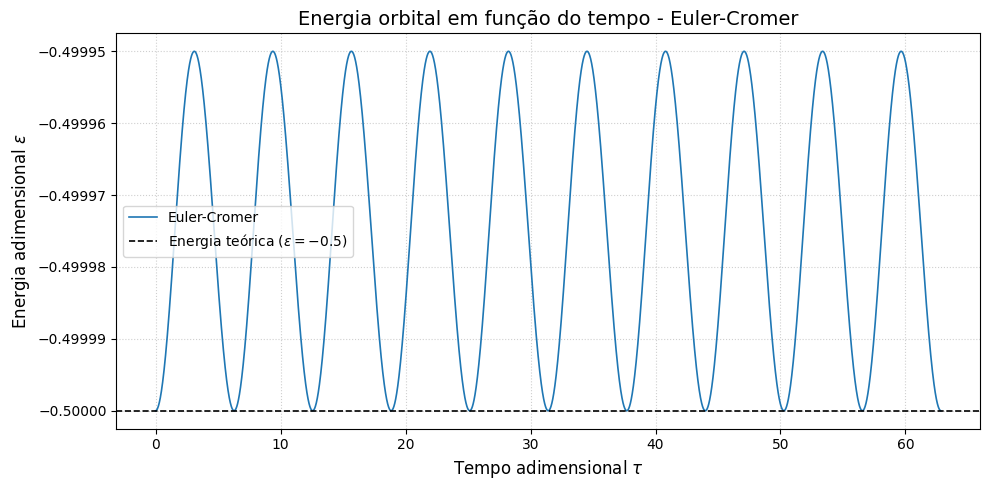
\includegraphics[width=0.9\textwidth]
    {tarefa-1d-grafico-1.png}
    \caption{Energia orbital adimensional em função do tempo para o método de Euler-Cromer. A linha tracejada representa a energia teórica ($\varepsilon=-0,5$).}
    \label{fig:energia-euler-cromer}
\end{figure}

Observa-se que a energia apresenta oscilações periódicas em torno do valor teórico, permanecendo aproximadamente entre $-0,50000$ e $-0,49995$. Portanto, a variação máxima observável no gráfico é da ordem de $5\times10^{-5}$. Ao longo do intervalo de integração, não se identifica uma deriva secular apreciável, mas um comportamento oscilatório limitado em torno da energia teórica.

A Figura \ref{fig:energia-verlet} apresenta os resultados correspondentes ao método de Verlet.

\begin{figure}[htbp]
    \centering
    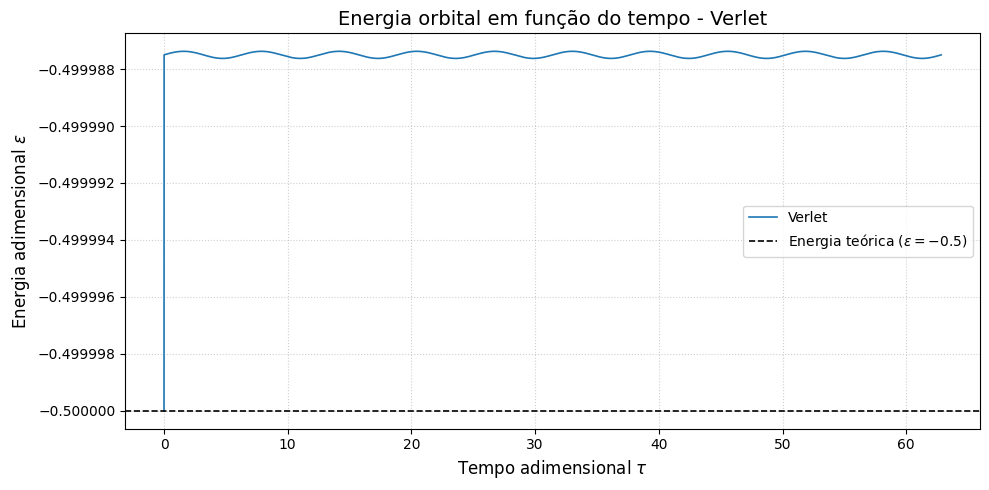
\includegraphics[width=0.9\textwidth]
    {tarefa-1d-grafico-2.png}
    \caption{Energia orbital adimensional em função do tempo para o método de Verlet. A linha tracejada representa a energia teórica ($\varepsilon=-0,5$).}
    \label{fig:energia-verlet}
\end{figure}

Nesse caso, observa-se uma descontinuidade no início da curva: a energia inicialmente registrada corresponde ao valor teórico $-0,5$, mas os valores seguintes passam a oscilar em torno de aproximadamente $-0,4999875$. Após esse desvio inicial, a energia permanece praticamente constante, apresentando oscilações de amplitude visualmente muito pequena e sem deriva secular apreciável ao longo da simulação.

Essa descontinuidade está relacionada ao procedimento de inicialização adotado no código. A primeira energia é calculada utilizando diretamente as condições iniciais, enquanto, a partir dos passos seguintes, as velocidades são reconstruídas por diferenças finitas centradas. Além disso, a segunda posição é obtida por uma aproximação de Euler. Portanto, a mudança observada no início da curva deve ser considerada ao interpretar o comportamento energético do método.

\vspace{0.5cm}
\hrule
\vspace{0.5cm}

\section{Problema 2: O problema de dois corpos -- órbitas limitadas}

\subsection{Item (a): Verificação das três leis de Kepler}

\subsubsection{Descrição do Problema}

Neste item, deve-se utilizar o método de Verlet para simular órbitas não circulares de planetas submetidos à atração gravitacional do Sol. O objetivo é investigar as condições em que as órbitas são fechadas ou não e, para os casos de órbitas fechadas, verificar numericamente as três leis de Kepler:

\begin{enumerate}
    \item Os planetas descrevem órbitas elípticas, tendo o Sol em um dos focos.
    \item O segmento de reta que liga o planeta ao Sol varre áreas iguais em intervalos de tempo iguais.
    \item O quadrado do período orbital $T$ é proporcional ao cubo do semieixo maior $a$, de modo que $T^2/a^3$ é constante para os diferentes planetas.
\end{enumerate}

% ORIENTAÇÕES À IA — ESTRATÉGIA DE SOLUÇÃO
% Leia o código F77 e explique como são escolhidas as condições iniciais não circulares e como o método de Verlet integra a órbita em unidades adimensionais.
% Para a primeira lei, descreva como a trajetória é registrada e como se identifica ou verifica sua compatibilidade com uma elipse com o Sol em um foco. Não afirme que houve ajuste de elipse se o código não o realiza.
% Para a segunda lei, explique como a área varrida é calculada em intervalos de tempo iguais, caso esteja implementado: explicite o método geométrico ou numérico usado e como os intervalos são escolhidos.
% Para a terceira lei, descreva como o período T e o semieixo maior a são obtidos para cada órbita e como se calcula T²/a³. Diferencie valores fornecidos de valores medidos numericamente.
% Informe os passos temporais, tempos de simulação, critérios de identificação do período e arquivos de saída efetivamente utilizados.
\subsubsection{Estratégia de Solução}

A simulação do movimento planetário é realizada utilizando o método de Verlet nas unidades adimensionais adotadas no projeto. A aceleração gravitacional do planeta, considerando o Sol fixo na origem, é dada por

\begin{equation}
    \vec{a}(\tau)=-\frac{\vec{\rho}(\tau)}{\rho(\tau)^3},
\end{equation}

em que $\vec{\rho}=(\rho_x,\rho_y)$ representa a posição do planeta e $\rho=|\vec{\rho}|$ é sua distância ao Sol.

A integração numérica é realizada pela equação de recorrência de Verlet:

\begin{equation}
    \vec{\rho}_{i+1}
    =
    2\vec{\rho}_i-\vec{\rho}_{i-1}
    -
    \frac{\vec{\rho}_i}{\rho_i^3}\Delta\tau^2.
\end{equation}

Assim como nos itens anteriores, são necessárias duas posições iniciais. A segunda posição é estimada pelo método de Euler:

\begin{equation}
    \vec{\rho}_1=
    \vec{\rho}_0+\vec{\upsilon}_0\Delta\tau.
\end{equation}

As velocidades são reconstruídas por diferenças finitas centradas:

\begin{equation}
    \vec{\upsilon}_i=
    \frac{\vec{\rho}_{i+1}-\vec{\rho}_{i-1}}
    {2\Delta\tau}.
\end{equation}

\paragraph{Condições iniciais e classificação das órbitas}

Para investigar diferentes tipos de trajetórias, foram mantidas as mesmas condições iniciais de posição e velocidade radial:

\begin{equation}
    \vec{\rho}_0=(1,0),
    \qquad
    \upsilon_{x,0}=0.
\end{equation}

A velocidade tangencial inicial $\upsilon_{y,0}$ foi variada em cinco casos:

\begin{equation}
    \upsilon_{y,0}\in
    \left\{
    1,1;\;
    1,2;\;
    1,3;\;
    \sqrt{2};\;
    1,5
    \right\}.
\end{equation}

A classificação das trajetórias é realizada a partir da energia mecânica específica adimensional, calculada pela função auxiliar \texttt{energia}:

\begin{equation}
    \varepsilon=
    \frac{1}{2}
    \left(\upsilon_x^2+\upsilon_y^2\right)
    -\frac{1}{\sqrt{\rho_x^2+\rho_y^2}}.
\end{equation}

Para as condições iniciais adotadas, como $\rho_0=1$ e $\upsilon_{x,0}=0$, a energia inicial assume a forma

\begin{equation}
    \varepsilon_0=
    \frac{\upsilon_{y,0}^2}{2}-1.
\end{equation}

Dessa maneira, energias negativas correspondem a órbitas elípticas, energia nula corresponde a uma trajetória parabólica e energias positivas correspondem a trajetórias hiperbólicas.

Para os casos elípticos, o semieixo maior é determinado a partir da energia mecânica inicial, utilizando a relação

\begin{equation}
    a=-\frac{1}{2\varepsilon_0}.
\end{equation}

\paragraph{Verificação da primeira lei de Kepler}

A primeira lei de Kepler é investigada pela representação gráfica das trajetórias obtidas numericamente. Para cada velocidade inicial, são armazenadas as componentes da posição do planeta ao longo do tempo, permitindo construir os gráficos de $\rho_y$ em função de $\rho_x$.

A análise consiste em verificar se as trajetórias limitadas apresentam formato elíptico e se o Sol, localizado na origem do sistema de coordenadas, ocupa uma das posições focais. Não é realizado ajuste geométrico de elipses: a verificação é feita diretamente pela observação das trajetórias calculadas.

\paragraph{Verificação da segunda lei de Kepler}

A segunda lei de Kepler é investigada por meio do cálculo acumulado da área varrida pelo vetor posição do planeta. Em cada passo temporal, a contribuição incremental de área é aproximada por

\begin{equation}
    \Delta A_i=
    \frac{\Delta\tau}{2}
    \left(
    \rho_{x,i}\upsilon_{y,i}
    -
    \rho_{y,i}\upsilon_{x,i}
    \right).
\end{equation}

A área acumulada é, portanto,

\begin{equation}
    A_n=
    \sum_{i=1}^{n}\Delta A_i.
\end{equation}

Esse procedimento é implementado diretamente pela variável \texttt{area} no programa. Para verificar a segunda lei, são construídos gráficos de $A(\tau)$ em função do tempo adimensional. A linearidade dessa relação indica que a área varrida cresce proporcionalmente ao tempo, correspondendo a uma velocidade areolar aproximadamente constante.

A comparação é realizada para as três trajetórias elípticas, considerando os mesmos passos temporais e intervalos de integração.

\paragraph{Verificação da terceira lei de Kepler}

A terceira lei de Kepler é investigada por meio da comparação entre o período orbital e o semieixo maior de cada uma das três órbitas elípticas.

O período é identificado numericamente pelo cruzamento do planeta com o eixo $x$ positivo, considerando a passagem de $\rho_y<0$ para $\rho_y\geq 0$, com $\rho_x>0$. O primeiro cruzamento que satisfaz essas condições após o início da simulação é utilizado como estimativa do período orbital.

A partir dos valores de $T$ e $a$, calcula-se a razão

\begin{equation}
    \frac{T^2}{a^3}.
\end{equation}

Nas unidades adimensionais adotadas, com $GM_{\odot}=1$, espera-se que essa razão seja constante e igual a

\begin{equation}
    \frac{T^2}{a^3}=4\pi^2.
\end{equation}

\paragraph{Parâmetros da simulação}

Todas as trajetórias são calculadas com passo temporal constante

\begin{equation}
    \Delta\tau=0,001
\end{equation}

e tempo máximo de integração

\begin{equation}
    \tau_{\max}=12\pi.
\end{equation}

O número de passos é determinado por

\begin{equation}
    N=\operatorname{int}
    \left(\frac{\tau_{\max}}{\Delta\tau}\right)
    =37699.
\end{equation}

Para cada uma das cinco condições iniciais, o programa gera um arquivo de saída denominado \texttt{tarefa-2a-saida-i.dat}, em que $i$ identifica a simulação. Os arquivos contêm seis colunas: tempo adimensional, componentes da posição, componentes da velocidade e área acumulada.

Ao término de cada simulação, o programa também apresenta o período orbital, o semieixo maior e a razão $T^2/a^3$, quando um período é identificado. Para as trajetórias parabólica e hiperbólica, nas quais não é identificado um período orbital no intervalo simulado, esses valores não são apresentados.

\begin{lstlisting}[
style=fortranstyle
]
      program tarefa2a
      ! O problema de dois corpos: órbitas limitadas com método de Verlet.
      ! Verifica as condições que geram órbitas fechadas
      ! Verifica as 3 leis de Kepler para órbitas elípticas.
      ! Utiliza-se a 3a Lei de Kepler GM = 4pi^2 UA^3 ano^(-2).
      ! Grandezas adimensionais rho = r/UA, tau = 2pi*t/ano, v = v/(2pi*UA/ano).
      ! Toma-se o Sol como origem estática e a Terra como corpo em órbita.

      implicit none

      character(30) filename
      integer*4 i
      real*8 taumax, dtau
      real*8 rx(50000), ry(50000), vx(50000), vy(50000), r(50000)
      real*8 pi
      parameter (pi = 3.14159265358979323d0)

      ! Condições iniciais adimensionais
      rx(1) = 1.0d0 ! posição inicial no eixo x
      ry(1) = 0.0d0 ! posição inicial no eixo y
      vx(1) = 0.0d0 ! velocidade inicial no eixo x

      ! Parâmetros da simulação
      taumax = 12.0d0 * pi ! Tempo adimensional máximo
      dtau = 0.001d0 ! passo de tempo adimensional

      ! Varia a vy(1) para gerar 3 elipses, 1 parábola e 1 hipérbole
      do i = 1,5
        if (i .le. 3) then ! 3 elipses
          vy(1) = 1.0d0 + 0.1d0*dble(i)
        else if (i .eq. 4) then ! parábola
          vy(1) = sqrt(2.0d0)
        else ! hipérbole
          vy(1) = 1.5d0
        end if

        write(filename, '(A,I1,A)') 'tarefa-2a-saida-', i, '.dat'

        call simulacao_orbita(
     &       filename, rx, ry, vx, vy, r, dtau, taumax)
      end do

      end program

      subroutine simulacao_orbita(
     &   filename, rx, ry, vx, vy, r, dtau, taumax)
      ! Simulação via método de Verlet
      ! Retorna tau, rx, ry, vx, vy, area
      implicit none
      character(30) filename
      real*8 rx(50000), ry(50000), vx(50000), vy(50000), r(50000)
      real*8 area, periodo
      real*8 tau, dtau, taumax
      real*8 energia_inicial, a
      real*8 energia
      integer*4 i, nsteps

      energia_inicial = energia(rx(1), ry(1), vx(1), vy(1))
      a = - 1.0d0 / (2.0d0 * energia_inicial) ! semieixo maior da órbita elíptica

      ! Número de passos da simulação
      nsteps = int(taumax/dtau)

      ! Para o método de Verlet, precisamos de uma segunda posição inicial
      ! Calculamos os valores de rx(1), ry(1), vx(1), vy(1)
      ! por meio do método de Euler para calcular a posição do passo i=2
      open(10, file=filename) ! Posições e velocidades

      area = 0.0d0
      periodo = -1.0d0 ! Inicializa o período como -1 para indicar que ainda não foi calculado

      write(10,*) 0.0d0, rx(1), ry(1), vx(1), vy(1), area

      rx(2) = rx(1) + vx(1)*dtau
      ry(2) = ry(1) + vy(1)*dtau
      do i = 2, nsteps

        ! Atualização da distância
        r(i) = sqrt(rx(i)**2 + ry(i)**2)

        ! Atualização das posições
        rx(i+1) = 2.0d0*rx(i) - rx(i-1) - (rx(i)/r(i)**3)*dtau**2
        ry(i+1) = 2.0d0*ry(i) - ry(i-1) - (ry(i)/r(i)**3)*dtau**2

        ! Atualização das velocidades
        vx(i) = (rx(i+1) - rx(i-1))/(2.0d0*dtau)
        vy(i) = (ry(i+1) - ry(i-1))/(2.0d0*dtau)

        ! Cálculo da área varrida pelo vetor posição
        area = area + dtau * 0.5d0 * (rx(i)*vy(i) - ry(i)*vx(i))

        tau = (i-1)*dtau
        write(10,*) tau, rx(i), ry(i), vx(i), vy(i), area

        ! Calcula o período da órbita quando a posição cruza o eixo x positivo
        if (ry(i-1) < 0.0d0 .and.
     &      ry(i) >= 0.0d0 .and.
     &      rx(i) > 0.0d0 .and.
     &      periodo .lt. 0.0d0) then
            periodo = tau
        end if

      end do

      if (periodo .gt. 0.0d0) then
        print *, 'Periodo da orbita: ', periodo
        print *, 'Semieixo maior da orbita: ', a
        print *, 'T^2/a^3: ', periodo**2 / a**3
      else
        print *, 'A orbita nao eh fechada => periodo nao definido.'
      end if

      close(10)
      end subroutine

      function energia(rx, ry, vx, vy)
      ! Calcula a energia total (cinética + potencial) de um corpo em órbita
      ! em torno de um corpo central, dado a posição (rx, ry) e velocidade (vx, vy)
      ! Unidade: GMm/UA, onde m é a massa do planeta
      
        implicit none
        real*8 rx, ry, vx, vy
        real*8 energia

        ! Energia cinética
        energia = 0.5d0 * (vx**2 + vy**2)

        ! Energia potencial gravitacional
        energia = energia - 1.0d0 / sqrt(rx**2 + ry**2)

      return
      end function
\end{lstlisting}


% ORIENTAÇÕES À IA — RESULTADOS OBTIDOS
% Apresente as trajetórias calculadas e discuta, para cada caso, se os dados indicam órbitas fechadas ou desvios em relação ao fechamento esperado.
% Analise a primeira lei com base na forma das trajetórias e na posição do Sol. Para a segunda, compare as áreas varridas em intervalos iguais e quantifique diferenças se os dados permitirem.
% Apresente T, a e T²/a³ para os casos analisados, esclarecendo como cada grandeza foi obtida. Compare a constância da razão entre planetas e com o valor esperado nas unidades adotadas, quando aplicável.
% Discuta limitações numéricas e diferenças entre fechamento visual e periodicidade efetiva.
\subsubsection{Resultados Obtidos}

\paragraph{Primeira lei de Kepler}

A Figura \ref{fig:orbitas-verlet} apresenta as trajetórias obtidas numericamente pelo método de Verlet para as cinco velocidades tangenciais iniciais consideradas.

\begin{figure}[htbp]
    \centering
    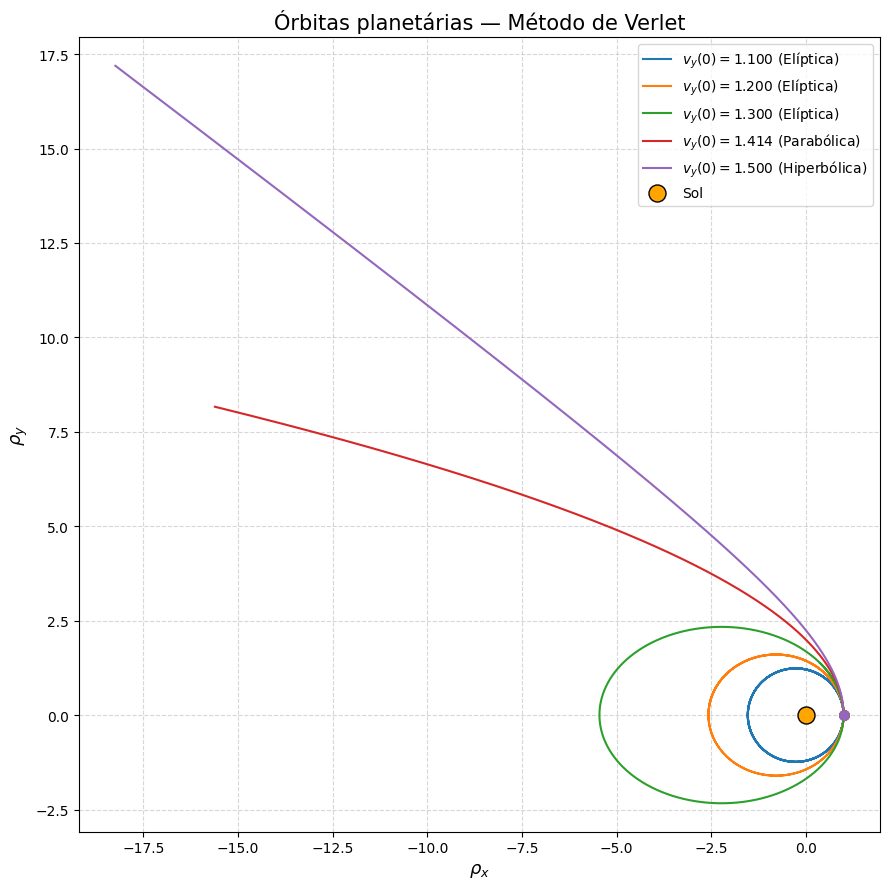
\includegraphics[width=0.9\textwidth]
    {tarefa-2a-grafico-1.png}
    \caption{Trajetórias planetárias obtidas pelo método de Verlet para diferentes velocidades tangenciais iniciais.}
    \label{fig:orbitas-verlet}
\end{figure}

Observa-se que, para as velocidades iniciais $\upsilon_{y,0}=1,1$, $\upsilon_{y,0}=1,2$ e $\upsilon_{y,0}=1,3$, são obtidas trajetórias elípticas fechadas, com o Sol localizado na origem, em uma das posições focais das elipses. Portanto, esses resultados são compatíveis com a primeira lei de Kepler.

Para compreender a diferença entre as trajetórias, pode-se analisar a energia mecânica inicial de cada caso. Como a posição inicial é $(1,0)$ e a velocidade inicial possui apenas componente na direção $y$, obtêm-se as seguintes classificações:

\begin{equation}
    \begin{aligned}
        \upsilon_{y,0}=1,1
        &\Rightarrow \varepsilon_0=-0,395,\\
        \upsilon_{y,0}=1,2
        &\Rightarrow \varepsilon_0=-0,280,\\
        \upsilon_{y,0}=1,3
        &\Rightarrow \varepsilon_0=-0,155,\\
        \upsilon_{y,0}=\sqrt{2}
        &\Rightarrow \varepsilon_0=0,\\
        \upsilon_{y,0}=1,5
        &\Rightarrow \varepsilon_0=0,125.
    \end{aligned}
\end{equation}

Assim, as três primeiras condições iniciais correspondem a energias negativas e, consequentemente, a órbitas elípticas. Para $\upsilon_{y,0}=\sqrt{2}$, a energia inicial é nula, resultando em uma trajetória parabólica. Finalmente, para $\upsilon_{y,0}=1,5$, a energia é positiva, correspondendo a uma trajetória hiperbólica.

As duas últimas trajetórias são abertas e não retornam à configuração inicial durante a simulação. Dessa forma, não apresentam fechamento orbital, em concordância com a classificação obtida a partir da energia mecânica.

\paragraph{Segunda lei de Kepler}

A verificação da segunda lei de Kepler é apresentada na Figura \ref{fig:area-kepler}, que mostra a área acumulada varrida pelo vetor posição em função do tempo para as três órbitas elípticas.

\begin{figure}[htbp]
    \centering
    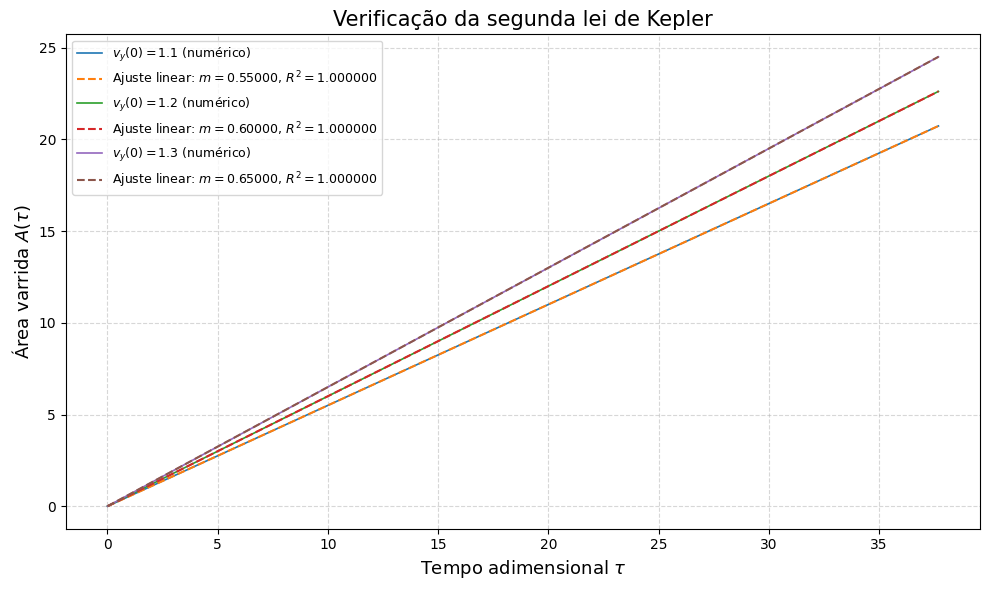
\includegraphics[width=0.9\textwidth]
    {tarefa-2a-grafico-2.png}
    \caption{Área varrida pelo vetor posição em função do tempo para diferentes velocidades tangenciais iniciais, com os respectivos ajustes lineares.}
    \label{fig:area-kepler}
\end{figure}

Observa-se uma dependência linear entre a área acumulada e o tempo para as três trajetórias. Os ajustes lineares apresentados no gráfico fornecem os seguintes coeficientes angulares:

\begin{equation}
    \begin{aligned}
        \upsilon_{y,0}=1,1
        &\Rightarrow m=0,55000,\\
        \upsilon_{y,0}=1,2
        &\Rightarrow m=0,60000,\\
        \upsilon_{y,0}=1,3
        &\Rightarrow m=0,65000.
    \end{aligned}
\end{equation}

Para os três ajustes, o coeficiente de determinação apresentado é $R^2=1,000000$, indicando concordância linear na precisão exibida pelo gráfico.

Esse comportamento pode ser compreendido a partir da velocidade areolar, dada por

\begin{equation}
    \frac{dA}{d\tau}
    =
    \frac{1}{2}
    \left(
    \rho_x\upsilon_y-\rho_y\upsilon_x
    \right).
\end{equation}

A quantidade entre parênteses corresponde ao momento angular específico em relação ao Sol, que permanece constante para uma força central. Portanto, espera-se uma velocidade areolar constante.

Como as condições iniciais são $\vec{\rho}_0=(1,0)$ e $\vec{\upsilon}_0=(0,\upsilon_{y,0})$, o momento angular específico inicial é igual a $\upsilon_{y,0}$. Assim, a velocidade areolar esperada é

\begin{equation}
    \frac{dA}{d\tau}
    =\frac{\upsilon_{y,0}}{2}.
\end{equation}

Consequentemente, os valores teóricos dos coeficientes angulares são, respectivamente, $0,55$, $0,60$ e $0,65$, coincidindo com os valores apresentados pelos ajustes lineares.

Portanto, os resultados numéricos estão em concordância com a segunda lei de Kepler: áreas iguais são varridas em intervalos de tempo iguais, uma vez que a área acumulada cresce linearmente com o tempo.

\paragraph{Terceira lei de Kepler}

Para verificar a terceira lei de Kepler, foram utilizados os semieixos maiores calculados a partir da energia mecânica inicial e os períodos identificados numericamente pelo cruzamento do eixo $x$ positivo.

Os resultados fornecidos pelo programa para as três órbitas elípticas estão organizados na Tabela \ref{tab:terceira-lei}.

\begin{table}[htbp]
    \centering
    \caption{Semieixos maiores, períodos orbitais e razões $T^2/a^3$ obtidos numericamente.}
    \label{tab:terceira-lei}
    \begin{tabular}{c c c c}
        \hline
        $\upsilon_{y,0}$ & $a$ & $T$ & $T^2/a^3$\\
        \hline
        $1,1$ & $1,265823$ & $8,949$ & $39,484832$\\
        $1,2$ & $1,785714$ & $14,994$ & $39,481995$\\
        $1,3$ & $3,225806$ & $36,404$ & $39,480559$\\
        \hline
    \end{tabular}
\end{table}

Observa-se que a razão $T^2/a^3$ apresenta valores praticamente constantes para as três órbitas. Para comparação, o valor teórico esperado nas unidades adimensionais utilizadas é

\begin{equation}
    4\pi^2\approx39,478418.
\end{equation}

As diferenças relativas entre os valores numéricos e o resultado teórico são aproximadamente $0,0162\%$, $0,0091\%$ e $0,0054\%$, respectivamente.

A pequena discrepância observada pode ser associada às aproximações numéricas utilizadas na integração e na determinação dos períodos. Em particular, o período é identificado pelo primeiro passo em que ocorre o cruzamento do eixo $x$ positivo, sem interpolação entre os instantes discretizados. Portanto, sua determinação possui resolução temporal limitada pelo passo $\Delta\tau=0,001$.

Para as trajetórias parabólica e hiperbólica, o programa não identifica um cruzamento que satisfaça o critério estabelecido durante o intervalo de integração. Consequentemente, não é atribuído um período orbital a esses casos, e a razão $T^2/a^3$ não é calculada.

Dessa forma, os resultados das três órbitas elípticas apresentam boa concordância com a terceira lei de Kepler, demonstrando que a razão entre o quadrado do período e o cubo do semieixo maior permanece aproximadamente constante.

\subsection{Item (b): Órbitas sob forças centrais com diferentes expoentes (opcional)}

\subsubsection{Descrição do Problema}

Neste item opcional, propõe-se investigar numericamente órbitas limitadas sob a ação de forças centrais da forma

\begin{equation}
    \vec{F}=-\rho^{\phi}\hat{\rho},
\end{equation}

em que $\phi$ é um expoente variável. Deve-se verificar que, para $\phi=1$, correspondente ao oscilador harmônico, e para $\phi=-2$, correspondente ao problema de Kepler, as órbitas limitadas são fechadas, não se restringindo aos casos de órbitas circulares.

% ORIENTAÇÕES À IA — ESTRATÉGIA DE SOLUÇÃO
% Consulte o código F77 e identifique como a força central F = -ρ^φ r̂ é implementada, inclusive o sinal, a direção radial, a dependência em ρ e o papel do expoente φ.
% Apresente a aceleração e as equações discretizadas utilizadas pelo integrador. Verifique se a constante multiplicativa da força é unitária ou possui outro valor no código.
% Descreva como φ é variado, quais condições iniciais são mantidas ou modificadas, qual passo temporal e intervalo de integração são empregados e como as trajetórias são armazenadas.
% Explique como o programa ou a análise identifica o caráter limitado e o fechamento das órbitas. Não atribua ao código um cálculo de período ou excentricidade que não exista.
\subsubsection{Estratégia de Solução}

O movimento do planeta é integrado numericamente pelo método de Verlet, considerando forças centrais da forma

\begin{equation}
    \vec{F}=-\rho^\phi\hat{\rho},
\end{equation}

em que $\rho$ representa a distância do planeta à origem, $\hat{\rho}$ é o vetor unitário na direção radial e $\phi$ é o expoente que determina a dependência da força com a distância.

Como a massa está normalizada nas unidades adimensionais adotadas, a aceleração possui a mesma expressão numérica da força. Escrevendo a aceleração em componentes cartesianas, obtém-se

\begin{equation}
    a_x=-\frac{\rho_x}{\rho^{1-\phi}},
    \qquad
    a_y=-\frac{\rho_y}{\rho^{1-\phi}},
\end{equation}

em que

\begin{equation}
    \rho=\sqrt{\rho_x^2+\rho_y^2}.
\end{equation}

A expressão corresponde à implementação da função auxiliar \texttt{aceleracao}, que recebe o expoente $\phi$, a componente da posição e a distância total ao centro de força. Observa-se que a constante multiplicativa da força é unitária, não havendo outro parâmetro de intensidade no código.

Foram considerados dois casos particulares:

\begin{equation}
    \phi=-2
    \quad\Longrightarrow\quad
    \vec{F}=-\frac{\hat{\rho}}{\rho^2},
\end{equation}

correspondente à força gravitacional do problema de Kepler, e

\begin{equation}
    \phi=1
    \quad\Longrightarrow\quad
    \vec{F}=-\rho\hat{\rho}=-\vec{\rho},
\end{equation}

correspondente à força restauradora do oscilador harmônico.

\paragraph{Integração pelo método de Verlet}

A evolução temporal das posições é calculada utilizando a equação de recorrência de Verlet:

\begin{equation}
    \vec{\rho}_{i+1}
    =
    2\vec{\rho}_i-\vec{\rho}_{i-1}
    +
    \vec{a}(\vec{\rho}_i)\Delta\tau^2.
\end{equation}

Em componentes cartesianas, as atualizações implementadas são

\begin{equation}
    \rho_{x,i+1}
    =
    2\rho_{x,i}-\rho_{x,i-1}
    +
    a_x(\rho_{x,i},\rho_i)\Delta\tau^2,
\end{equation}

\begin{equation}
    \rho_{y,i+1}
    =
    2\rho_{y,i}-\rho_{y,i-1}
    +
    a_y(\rho_{y,i},\rho_i)\Delta\tau^2.
\end{equation}

Como o método necessita de duas posições iniciais, a segunda posição é calculada por uma aproximação de Euler:

\begin{equation}
    \vec{\rho}_1=
    \vec{\rho}_0+\vec{\upsilon}_0\Delta\tau.
\end{equation}

Diferentemente dos itens anteriores, nesta implementação são armazenadas apenas as componentes da posição, não sendo realizada a reconstrução das velocidades durante a integração.

\paragraph{Condições iniciais e parâmetros da simulação}

Em todas as simulações, são mantidas as mesmas condições iniciais de posição e velocidade radial:

\begin{equation}
    \vec{\rho}_0=(1,0),
    \qquad
    \upsilon_{x,0}=0.
\end{equation}

Para investigar diferentes trajetórias, são utilizadas cinco velocidades tangenciais iniciais:

\begin{equation}
    \upsilon_{y,0}\in
    \{0,70;\;0,85;\;1,00;\;1,10;\;1,20\}.
\end{equation}

Primeiramente, são realizadas cinco simulações com $\phi=-2$, uma para cada velocidade inicial. Em seguida, o procedimento é repetido para $\phi=1$, mantendo-se os mesmos valores de velocidade. Portanto, são obtidas dez trajetórias no total.

O intervalo e o passo temporal são iguais para todas as simulações:

\begin{equation}
    \tau_{\max}=12\pi,
\end{equation}

\begin{equation}
    \Delta\tau=0,001.
\end{equation}

O número de passos é calculado por

\begin{equation}
    N=\operatorname{int}
    \left(\frac{\tau_{\max}}{\Delta\tau}\right)
    =37699.
\end{equation}

As posições são registradas nos arquivos \texttt{tarefa-2b-saida-i.dat}, com $i$ variando de 1 a 10. Cada arquivo contém três colunas: tempo adimensional, posição na direção $x$ e posição na direção $y$.

\paragraph{Identificação do período orbital}

O programa também implementa um procedimento para estimar o período orbital. Para isso, verifica quando a posição do planeta cruza o eixo $x$ positivo, considerando simultaneamente as condições

\begin{equation}
    \rho_{y,i-1}<0,
    \qquad
    \rho_{y,i}\geq 0,
    \qquad
    \rho_{x,i}>0.
\end{equation}

Quando essas condições são satisfeitas pela primeira vez, o instante correspondente é registrado como período da órbita. Caso não seja identificado um cruzamento durante a simulação, o programa informa que o período não foi determinado.

Esse procedimento fornece uma estimativa numérica do período a partir de um cruzamento do eixo, não sendo realizado um teste explícito de coincidência entre as posições e velocidades finais e iniciais. A identificação do fechamento das trajetórias é, portanto, complementada pela análise visual dos gráficos.

\begin{lstlisting}[
style=fortranstyle
]
      program tarefa2b
      ! O problema de dois corpos: órbitas limitadas com método de Verlet.
      ! Gera trajetórias sob forças centrais da forma F F = - rho^phi.
      ! Mostra exemplos com phi = 1 (elástica) e phi = -2 (Kepler)
      ! Utiliza-se a 3a Lei de Kepler GM = 4pi^2 UA^3 ano^(-2).
      ! Grandezas adimensionais rho = r/UA, tau = 2pi*t/ano, v = v/(2pi*UA/ano).
      ! Toma-se o Sol como origem estática e a Terra como corpo em órbita.

      implicit none

      character(30) filename
      integer*4 i
      real*8 phi
      real*8 taumax, dtau
      real*8 rx(50000), ry(50000), vx, vy, r(50000)
      real*8 velocidades(5)
      real*8 pi
      parameter (pi = 3.14159265358979323d0)

      ! Condições iniciais adimensionais
      rx(1) = 1.0d0 ! posição inicial no eixo x
      ry(1) = 0.0d0 ! posição inicial no eixo y
      vx = 0.0d0 ! velocidade inicial no eixo x

      ! Parâmetros da simulação
      taumax = 12.0d0 * pi ! Tempo adimensional máximo
      dtau = 0.001d0 ! passo de tempo adimensional

      ! ! Varia a vy(1) para gerar trajetórias diferentes com diferentes forças centrais ! !

      ! Velocidades iniciais para diferentes órbitas
      velocidades(1) = 0.70d0
      velocidades(2) = 0.85d0
      velocidades(3) = 1.00d0
      velocidades(4) = 1.10d0
      velocidades(5) = 1.20d0

      phi = -2.0d0 ! Kepler: F ~ -1/r^2

      do i = 1,5
        vy = velocidades(i)

        write(filename, '(A,I0,A)')
     &       'tarefa-2b-saida-', i, '.dat'

        call simulacao_orbita(
     &       filename, phi, rx, ry, vx, vy, r, dtau, taumax)
      end do

      phi = 1.0d0 ! Oscilador harmônico: F ~ -r

      do i = 6,10
        vy = velocidades(i-5)

        write(filename, '(A,I0,A)')
     &       'tarefa-2b-saida-', i, '.dat'

        call simulacao_orbita(
     &       filename, phi, rx, ry, vx, vy, r, dtau, taumax)
      end do

      end program

      subroutine simulacao_orbita(
     &   filename, phi, rx, ry, vx, vy, r, dtau, taumax)
      ! Simulação de um corpo sofrendo força central da forma 
      ! F = - rho^phi pelo Sol via método de Verlet
      ! Retorna tau, rx, ry
      implicit none
      character(30) filename
      real*8 phi
      real*8 rx(50000), ry(50000), vx, vy, r(50000)
      real*8 periodo
      real*8 tau, dtau, taumax
      real*8 aceleracao
      integer*4 i, nsteps

      ! Número de passos da simulação
      nsteps = int(taumax/dtau)

      ! Para o método de Verlet, precisamos de uma segunda posição inicial
      ! Calculamos os valores de rx(1), ry(1), vx(1), vy(1)
      ! por meio do método de Euler para calcular a posição do passo i=2
      open(10, file=filename) ! Posições e velocidades

      periodo = -1.0d0 ! Inicializa o período como -1 para indicar que ainda não foi calculado

      write(10,*) 0.0d0, rx(1), ry(1)

      rx(2) = rx(1) + vx*dtau
      ry(2) = ry(1) + vy*dtau
      do i = 2, nsteps

        ! Atualização da distância
        r(i) = sqrt(rx(i)**2 + ry(i)**2)

        ! Atualização das posições
        rx(i+1) = 2.0d0*rx(i) - rx(i-1) +
     &   aceleracao(phi, rx(i), r(i))*dtau**2
        ry(i+1) = 2.0d0*ry(i) - ry(i-1) +
     &   aceleracao(phi, ry(i), r(i))*dtau**2

        tau = (i-1)*dtau
        write(10,*) tau, rx(i), ry(i)

        ! Calcula o período da órbita quando a posição cruza o eixo x positivo
        if (ry(i-1) < 0.0d0 .and.
     &      ry(i) >= 0.0d0 .and.
     &      rx(i) > 0.0d0 .and.
     &      periodo .lt. 0.0d0) then
            periodo = tau
        end if

      end do

      if (periodo .gt. 0.0d0) then
        print *, 'Periodo da orbita: ', periodo
      else
        print *, 'A orbita nao eh fechada => periodo nao definido.'
      end if

      close(10)
      end subroutine

      function aceleracao(phi, r_componente, r)
      ! aceleração na direção de r_componente oriunda de uma força central da forma F = - rho^phi 
      ! onde rho = r/UA, phi é o expoente da força central, r_componente é a componente da posição (rx ou ry)
      ! e r é a distância total (raiz quadrada da soma dos quadrados das componentes)
        implicit none
        real*8 phi, r_componente, r
        real*8 aceleracao
        aceleracao = - (r_componente / r**(-phi + 1.0d0))
      return
      end function

      function energia(rx, ry, vx, vy)
      ! Calcula a energia total (cinética + potencial) de um corpo em órbita
      ! em torno de um corpo central, dado a posição (rx, ry) e velocidade (vx, vy)
      ! Unidade: GMm/UA, onde m é a massa do planeta
      
        implicit none
        real*8 rx, ry, vx, vy
        real*8 energia

        ! Energia cinética
        energia = 0.5d0 * (vx**2 + vy**2)

        ! Energia potencial gravitacional
        energia = energia - 1.0d0 / sqrt(rx**2 + ry**2)

      return
      end function
\end{lstlisting}


% ORIENTAÇÕES À IA — RESULTADOS OBTIDOS
% Apresente as trajetórias para os expoentes efetivamente simulados, destacando separadamente φ = 1 e φ = -2 quando constarem nos resultados.
% Discuta se as órbitas observadas são limitadas e se aparentam fechar, apoiando a análise nos gráficos, nos períodos ou em medidas quantitativas disponíveis.
% Compare os comportamentos associados ao oscilador harmônico e ao problema de Kepler, sem generalizar para valores de φ que não tenham sido simulados.
\subsubsection{Resultados Obtidos}

A Figura \ref{fig:orbitas-forcas-centrais} apresenta as trajetórias obtidas numericamente para os dois potenciais considerados, utilizando diferentes velocidades tangenciais iniciais.

\begin{figure}[htbp]
    \centering
    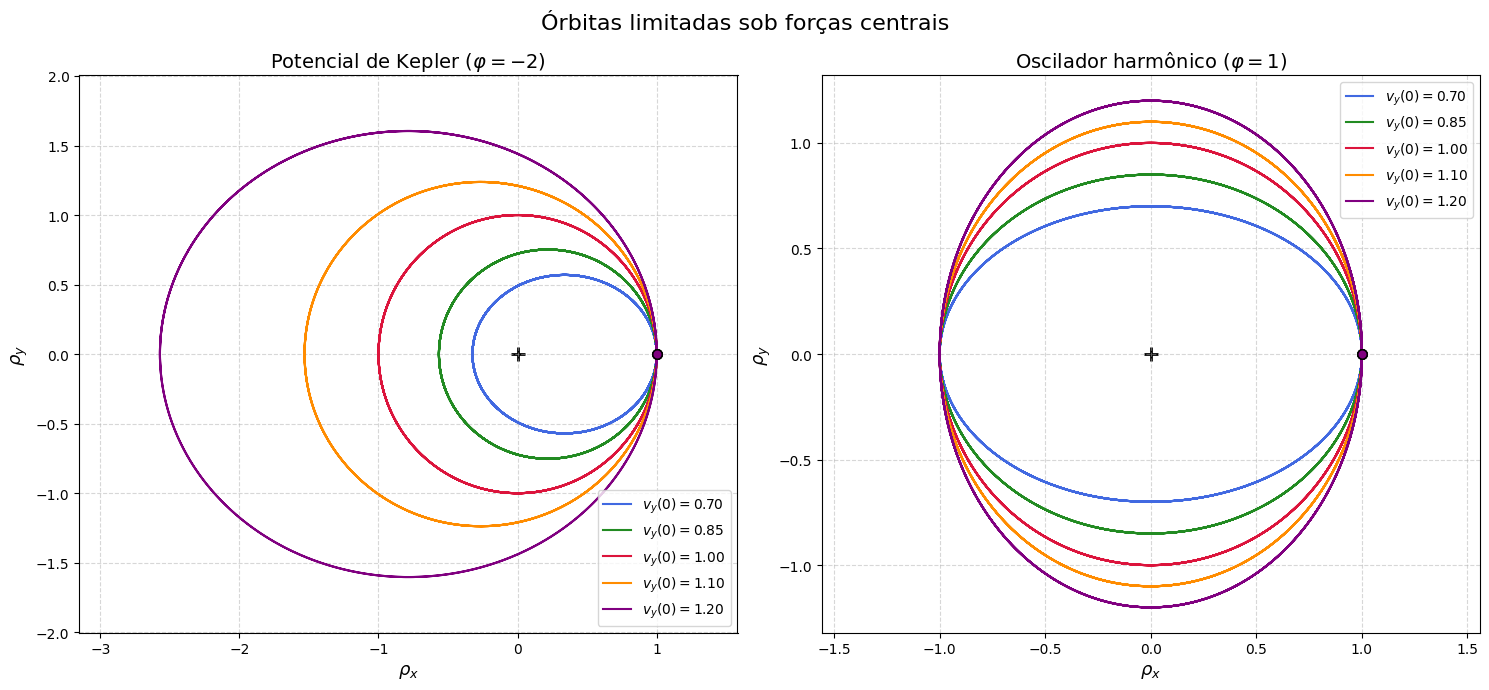
\includegraphics[width=\textwidth]
    {tarefa-2b-grafico-1.png}
    \caption{Trajetórias planetárias obtidas pelo método de Verlet para diferentes velocidades tangenciais iniciais, considerando o potencial de Kepler ($\phi=-2$) e o oscilador harmônico ($\phi=1$).}
    \label{fig:orbitas-forcas-centrais}
\end{figure}

\paragraph{Potencial de Kepler ($\phi=-2$)}

No caso do potencial de Kepler, observa-se que as cinco velocidades iniciais consideradas produzem trajetórias elípticas limitadas e fechadas no intervalo apresentado. Além disso, todas as elipses apresentam o Sol na origem do sistema de coordenadas, em uma de suas posições focais, em concordância com a primeira lei de Kepler.

Observa-se também que a geometria das órbitas depende da velocidade tangencial inicial. Para velocidades menores, as trajetórias apresentam menor extensão na direção radial, enquanto velocidades maiores produzem elipses progressivamente mais alongadas. Esse comportamento está relacionado à maior energia mecânica associada ao aumento da velocidade inicial.

A identificação numérica dos períodos foi realizada pelo critério de cruzamento do eixo $x$ positivo descrito anteriormente. Os resultados impressos pelo programa são apresentados na Tabela \ref{tab:periodos-kepler-harmonico}.

\paragraph{Oscilador harmônico ($\phi=1$)}

Para o oscilador harmônico, também são observadas cinco trajetórias limitadas e fechadas. Entretanto, diferentemente do potencial de Kepler, as órbitas são elipses centradas na origem, que corresponde ao centro da força restauradora.

A variação da velocidade tangencial inicial modifica a extensão das trajetórias na direção $y$, produzindo elipses com diferentes semieixos. Apesar dessas diferenças geométricas, todas as trajetórias apresentam aproximadamente o mesmo período.

Esse comportamento pode ser compreendido pelas equações diferenciais do oscilador harmônico, que, nas unidades adotadas, são

\begin{equation}
    \ddot{\rho}_x=-\rho_x,
    \qquad
    \ddot{\rho}_y=-\rho_y.
\end{equation}

Ambas as componentes apresentam frequência angular unitária. Assim, o período teórico é

\begin{equation}
    T=2\pi,
\end{equation}

independentemente da amplitude do movimento. Esse resultado é consistente com os períodos numéricos obtidos nas cinco simulações.

\paragraph{Comparação dos períodos}

Os períodos identificados numericamente para os dois potenciais estão organizados na Tabela \ref{tab:periodos-kepler-harmonico}.

\begin{table}[htbp]
    \centering
    \caption{Períodos orbitais identificados numericamente para os diferentes potenciais e velocidades tangenciais iniciais.}
    \label{tab:periodos-kepler-harmonico}
    \begin{tabular}{c c c}
        \hline
        $\upsilon_{y,0}$ &
        $T$ para $\phi=-2$ &
        $T$ para $\phi=1$ \\
        \hline
        $0,70$ & $3,387$ & $6,284$ \\
        $0,85$ & $4,352$ & $6,284$ \\
        $1,00$ & $6,284$ & $6,284$ \\
        $1,10$ & $8,949$ & $6,284$ \\
        $1,20$ & $14,994$ & $6,284$ \\
        \hline
    \end{tabular}
\end{table}

No potencial de Kepler, verifica-se que o período aumenta com a velocidade tangencial inicial. Esse comportamento está associado ao aumento da energia mecânica e, consequentemente, ao aumento do semieixo maior das órbitas elípticas.

Por outro lado, no oscilador harmônico, os cinco períodos identificados são iguais na precisão apresentada, correspondendo aproximadamente a $2\pi$. Portanto, os resultados confirmam numericamente a independência do período em relação à amplitude para esse potencial.

\subsection{Item (c): Investigação de órbitas ilimitadas e limitadas (opcional)}

\subsubsection{Descrição do Problema}

Neste item opcional, deve-se investigar a existência de órbitas ilimitadas, caracterizadas por $\rho\rightarrow\infty$ quando $\tau\rightarrow\infty$, para forças centrais com $\phi>0$. Também se propõe verificar a existência de órbitas limitadas para $\phi\leq -3$. O objetivo é realizar simulações variando o expoente $\phi$ e discutir os comportamentos orbitais observados.

% ORIENTAÇÕES À IA — ESTRATÉGIA DE SOLUÇÃO
% Leia o código F77 e explique como a variação do expoente φ é feita e como a força central correspondente é convertida em aceleração.
% Descreva as condições iniciais, o integrador, o passo temporal e o horizonte de simulação. Identifique quais grandezas são monitoradas para classificar uma órbita como limitada ou em expansão.
% Explique o critério operacional usado para reconhecer órbitas ilimitadas nos dados finitos e como o programa trata a condição ρ → ∞ quando τ → ∞. Ressalte que uma simulação finita fornece evidência numérica, não uma demonstração do limite matemático.
% Registre a faixa e os valores discretos de φ realmente investigados, bem como qualquer critério de parada ou limite numérico.
\subsubsection{Estratégia de Solução}

\paragraph{Condições iniciais e variação dos parâmetros}

Em todas as simulações, são mantidas as condições iniciais

\begin{equation}
    \vec{\rho}_0=(1,0),
    \qquad
    \upsilon_{x,0}=0.
\end{equation}

A investigação é dividida em dois conjuntos de simulações.

Inicialmente, são considerados expoentes positivos:

\begin{equation}
    \phi\in\{0,5;\;1;\;2;\;4\}.
\end{equation}

Para cada um desses expoentes, são utilizadas duas velocidades tangenciais iniciais:

\begin{equation}
    \upsilon_{y,0}\in\{1,0;\;2,0\}.
\end{equation}

Em seguida, são investigados os casos com $\phi\leq -3$, utilizando

\begin{equation}
    \phi\in\{-3;\;-4;\;-5\}
\end{equation}

e três velocidades tangenciais iniciais:

\begin{equation}
    \upsilon_{y,0}\in\{0,8;\;1,0;\;1,2\}.
\end{equation}

Dessa maneira, são realizadas oito simulações para $\phi>0$ e nove simulações para $\phi\leq-3$, totalizando dezessete trajetórias.

\paragraph{Parâmetros de integração e armazenamento}

Todas as simulações utilizam o mesmo passo temporal e intervalo de integração:

\begin{equation}
    \Delta\tau=0,001,
\end{equation}

\begin{equation}
    \tau_{\max}=12\pi.
\end{equation}

O número de passos é determinado por

\begin{equation}
    N=\operatorname{int}
    \left(\frac{\tau_{\max}}{\Delta\tau}\right)
    =37699.
\end{equation}

As posições são armazenadas nos arquivos \texttt{tarefa-2c-saida-i-j.dat}, em que os índices identificam o expoente considerado e a velocidade inicial utilizada. Cada arquivo contém três colunas: tempo adimensional, posição na direção $x$ e posição na direção $y$.

\paragraph{Critérios de acompanhamento das trajetórias}

A análise do comportamento orbital é realizada por meio das posições calculadas ao longo do tempo, posteriormente representadas em gráficos de $\rho_y$ em função de $\rho_x$. Dessa forma, é possível observar se as trajetórias permanecem em uma região limitada ou apresentam grandes deslocamentos em relação à origem.

O código também verifica a ocorrência de aproximação excessiva do centro de força. Quando a distância satisfaz

\begin{equation}
    \rho<0,2,
\end{equation}

a integração é interrompida, sendo impressa uma mensagem indicando a aproximação excessiva do Sol central.

Adicionalmente, o programa verifica se ocorre um cruzamento do eixo $x$ positivo, por meio das condições

\begin{equation}
    \rho_{y,i-1}<0,
    \qquad
    \rho_{y,i}\geq0,
    \qquad
    \rho_{x,i}>0.
\end{equation}

Quando esse cruzamento é identificado, seu instante é registrado como período da órbita. Caso contrário, o programa informa que a órbita não é fechada e que o período não foi definido.

\begin{lstlisting}[
style=fortranstyle
]
      program tarefa2c
      ! O problema de dois corpos: órbitas com método de Verlet.
      ! Gera trajetórias sob forças centrais da forma F = - rho^phi.
      ! Mostra exemplos com phi > 0 e phi <= -3.
      ! Utiliza-se a 3a Lei de Kepler GM = 4pi^2 UA^3 ano^(-2).
      ! Grandezas adimensionais rho = r/UA, tau = 2pi*t/ano, v = v/(2pi*UA/ano).
      ! Toma-se o Sol como origem estática e a Terra como corpo em órbita.

      implicit none

      character(30) filename
      integer*4 i, j
      real*8 phi
      real*8 taumax, dtau
      real*8 rx(50000), ry(50000), vx, vy, r(50000)
      real*8 velocidades(5)
      real*8 expoentes(7)
      real*8 pi
      parameter (pi = 3.14159265358979323d0)

      ! Condições iniciais adimensionais
      rx(1) = 1.0d0 ! posição inicial no eixo x
      ry(1) = 0.0d0 ! posição inicial no eixo y
      vx = 0.0d0 ! velocidade inicial no eixo x

      ! Parâmetros da simulação
      taumax = 12.0d0 * pi ! Tempo adimensional máximo
      dtau = 0.001d0 ! passo de tempo adimensional

      ! ! Varia a vy(1) para gerar trajetórias diferentes com diferentes forças centrais ! !

      ! Velocidades iniciais para diferentes órbitas
      velocidades(1) = 0.80d0
      velocidades(2) = 1.00d0
      velocidades(3) = 1.20d0

      ! Expoentes das forças centrais
      expoentes(1) = 0.5d0
      expoentes(2) = 1.0d0
      expoentes(3) = 2.0d0
      expoentes(4) = 4.0d0
      expoentes(5) = -3.0d0
      expoentes(6) = -4.0d0
      expoentes(7) = -5.0d0

      ! Simulações para phi > 0
      do i = 1,4
        phi = expoentes(i)

        do j = 1,2
          if (j .eq. 1) then
            vy = 1.0d0
          else
            vy = 2.0d0
          end if

          write(filename, '(A,I1,A,I1,A)')
     &       'tarefa-2c-saida-', i, '-', j, '.dat'

          call simulacao_orbita(
     &       filename, phi, rx, ry, vx, vy, r, dtau, taumax)
        end do
      end do

      ! Simulações para phi <= -3
      do i = 5,7
        phi = expoentes(i)

        do j = 1,3
          vy = velocidades(j)

          write(filename, '(A,I1,A,I1,A)')
     &       'tarefa-2c-saida-', i, '-', j, '.dat'

          call simulacao_orbita(
     &       filename, phi, rx, ry, vx, vy, r, dtau, taumax)
        end do
      end do

      end program

      subroutine simulacao_orbita(
     &   filename, phi, rx, ry, vx, vy, r, dtau, taumax)
      ! Simulação de um corpo sofrendo força central da forma 
      ! F = - rho^phi pelo Sol via método de Verlet
      ! Retorna tau, rx, ry
      implicit none
      character(30) filename
      real*8 phi
      real*8 rx(50000), ry(50000), vx, vy, r(50000)
      real*8 periodo
      real*8 tau, dtau, taumax
      real*8 aceleracao
      integer*4 i, nsteps

      ! Número de passos da simulação
      nsteps = int(taumax/dtau)

      ! Para o método de Verlet, precisamos de uma segunda posição inicial
      ! Calculamos os valores de rx(1), ry(1), vx(1), vy(1)
      ! por meio do método de Euler para calcular a posição do passo i=2
      open(10, file=filename) ! Posições e velocidades

      periodo = -1.0d0 ! Inicializa o período como -1 para indicar que ainda não foi calculado

      write(10,*) 0.0d0, rx(1), ry(1)

      rx(2) = rx(1) + vx*dtau
      ry(2) = ry(1) + vy*dtau
      do i = 2, nsteps

        ! Atualização da distância
        r(i) = sqrt(rx(i)**2 + ry(i)**2)

        ! Interrompe a simulacao quando ocorre aproximacao
        ! excessiva do Sol central
        if (r(i) .lt. 0.2d0) then
          print *, 'Aproximacao excessiva do Sol central.'
          print *, 'phi = ', phi, ' vy = ', vy
          exit
        end if

        ! Atualização das posições
        rx(i+1) = 2.0d0*rx(i) - rx(i-1) +
     &   aceleracao(phi, rx(i), r(i))*dtau**2
        ry(i+1) = 2.0d0*ry(i) - ry(i-1) +
     &   aceleracao(phi, ry(i), r(i))*dtau**2

        tau = (i-1)*dtau
        write(10,*) tau, rx(i), ry(i)

        ! Calcula o período da órbita quando a posição cruza o eixo x positivo
        if (ry(i-1) < 0.0d0 .and.
     &      ry(i) >= 0.0d0 .and.
     &      rx(i) > 0.0d0 .and.
     &      periodo .lt. 0.0d0) then
            periodo = tau
        end if

      end do

      if (periodo .gt. 0.0d0) then
        print *, 'Periodo da orbita: ', periodo
      else
        print *, 'A orbita nao eh fechada => periodo nao definido.'
      end if

      close(10)
      end subroutine

      function aceleracao(phi, r_componente, r)
      ! aceleração na direção de r_componente oriunda de uma força central da forma F = - rho^phi 
      ! onde rho = r/UA, phi é o expoente da força central, r_componente é a componente da posição (rx ou ry)
      ! e r é a distância total (raiz quadrada da soma dos quadrados das componentes)
        implicit none
        real*8 phi, r_componente, r
        real*8 aceleracao
        aceleracao = - (r_componente / r**(-phi + 1.0d0))
      return
      end function

      function energia(rx, ry, vx, vy)
      ! Calcula a energia total (cinética + potencial) de um corpo em órbita
      ! em torno de um corpo central, dado a posição (rx, ry) e velocidade (vx, vy)
      ! Unidade: GMm/UA, onde m é a massa do planeta
      
        implicit none
        real*8 rx, ry, vx, vy
        real*8 energia

        ! Energia cinética
        energia = 0.5d0 * (vx**2 + vy**2)

        ! Energia potencial gravitacional
        energia = energia - 1.0d0 / sqrt(rx**2 + ry**2)

      return
      end function
\end{lstlisting}


% ORIENTAÇÕES À IA — RESULTADOS OBTIDOS
% Organize os resultados por valor de φ e descreva quais trajetórias permanecem em uma região limitada e quais apresentam crescimento persistente da distância durante o intervalo simulado.
% Discuta separadamente os casos φ > 0 e φ ≤ -3, indicando quais exemplos foram de fato calculados e se os resultados são compatíveis com a proposta do item.
% Aponte limitações da classificação por tempo finito e evite afirmar comportamento assintótico como prova matemática.
\subsubsection{Resultados Obtidos}

A Figura \ref{fig:orbitas-diferentes-forcas} apresenta as trajetórias obtidas numericamente para os expoentes positivos e para os expoentes menores ou iguais a $-3$, considerando as diferentes velocidades tangenciais iniciais.

\begin{figure}[htbp]
    \centering
    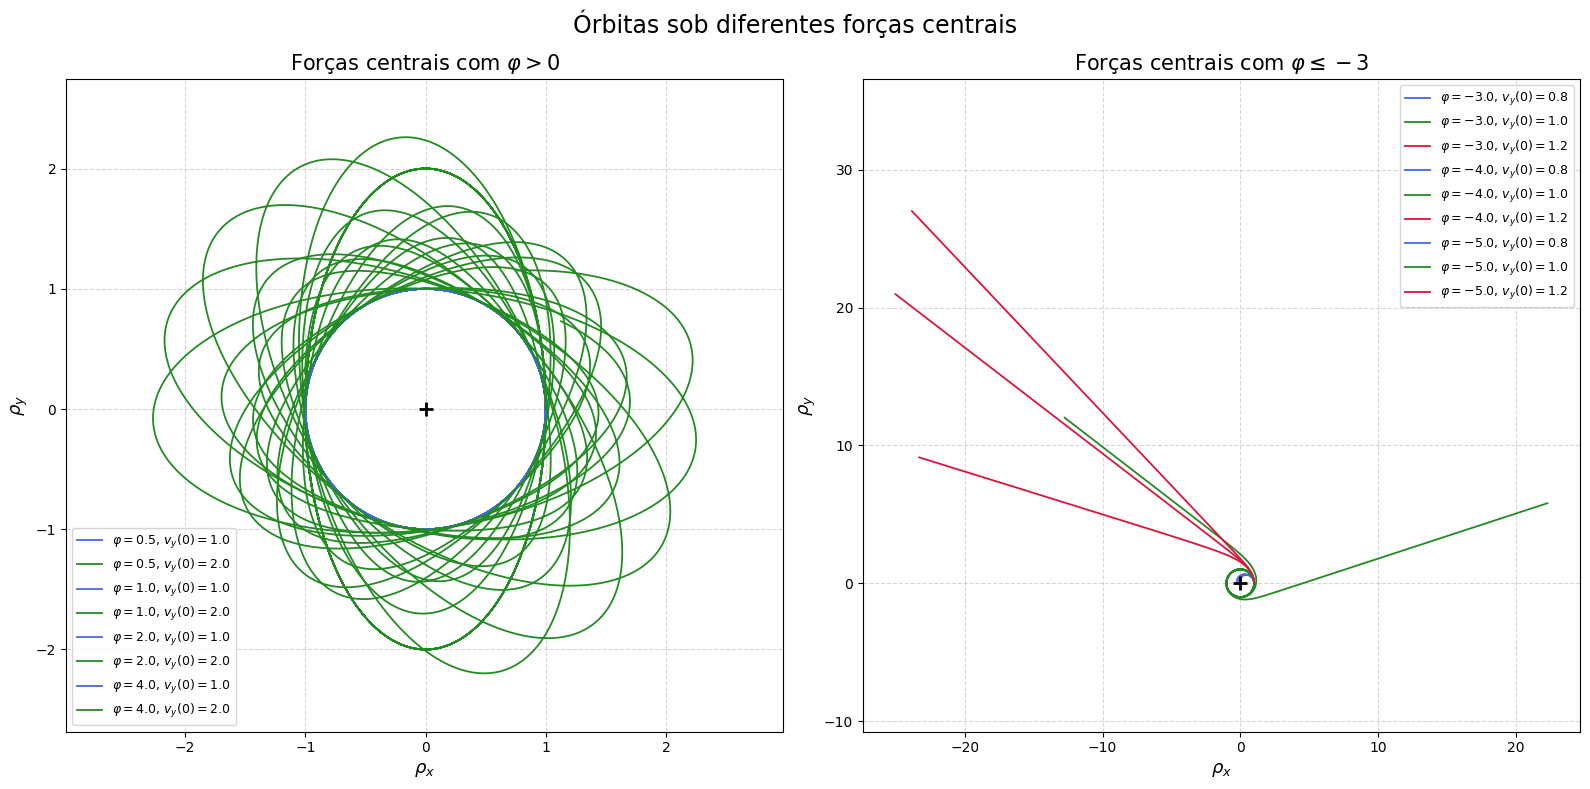
\includegraphics[width=\textwidth]
    {tarefa-2c-grafico-1.png}
    \caption{Trajetórias obtidas pelo método de Verlet para diferentes expoentes $\phi$ e velocidades tangenciais iniciais, considerando $\phi>0$ e $\phi\leq-3$.}
    \label{fig:orbitas-diferentes-forcas}
\end{figure}

\paragraph{Forças centrais com $\phi>0$}

Para os expoentes positivos investigados, $\phi=0,5$, $\phi=1$, $\phi=2$ e $\phi=4$, observa-se que as trajetórias permanecem confinadas a regiões limitadas do plano durante o intervalo de integração.

As diferentes velocidades tangenciais iniciais produzem trajetórias com geometrias distintas, embora todas permaneçam próximas à região central.

Os períodos identificados numericamente pelo programa para essas simulações são apresentados na Tabela \ref{tab:periodos-phi-positivo}.

\begin{table}[htbp]
    \centering
    \caption{Períodos identificados numericamente para os expoentes positivos.}
    \label{tab:periodos-phi-positivo}
    \begin{tabular}{c c c}
        \hline
        $\phi$ & $\upsilon_{y,0}$ & $T$ \\
        \hline
        $0,5$ & $1,0$ & $6,284$ \\
        $0,5$ & $2,0$ & $7,459$ \\
        $1,0$ & $1,0$ & $6,284$ \\
        $1,0$ & $2,0$ & $6,284$ \\
        $2,0$ & $1,0$ & $6,284$ \\
        $2,0$ & $2,0$ & $5,113$ \\
        $4,0$ & $1,0$ & $6,284$ \\
        $4,0$ & $2,0$ & $4,513$ \\
        \hline
    \end{tabular}
\end{table}

Os resultados mostram que o período identificado varia conforme o expoente da força central e a velocidade tangencial inicial. Entretanto, esses valores correspondem ao primeiro cruzamento subsequente do eixo $x$ positivo, não sendo necessariamente períodos de fechamento completo para trajetórias que apresentam precessão.

\paragraph{Forças centrais com $\phi\leq-3$}

Para os expoentes negativos, $\phi=-3$, $\phi=-4$ e $\phi=-5$, observa-se um comportamento significativamente diferente. As trajetórias apresentam maior sensibilidade às condições iniciais, com alguns casos exibindo grandes deslocamentos radiais e outros se aproximando excessivamente do centro de força.

Os demais resultados numéricos são apresentados na Tabela \ref{tab:periodos-phi-negativo}.

\begin{table}[htbp]
    \centering
    \caption{Resultados das simulações para os expoentes $\phi\leq-3$.}
    \label{tab:periodos-phi-negativo}
    \begin{tabular}{c c c}
        \hline
        $\phi$ & $\upsilon_{y,0}$ & Resultado \\
        \hline
        $-3$ & $0,8$ & Aproximação excessiva \\
        $-3$ & $1,0$ & Período não identificado \\
        $-3$ & $1,2$ & $T=6,304$ \\
        $-4$ & $0,8$ & Aproximação excessiva \\
        $-4$ & $1,0$ & Período não identificado \\
        $-4$ & $1,2$ & $T=6,573$ \\
        $-5$ & $0,8$ & Aproximação excessiva \\
        $-5$ & $1,0$ & $T=11,297$ \\
        $-5$ & $1,2$ & Período não identificado \\
        \hline
    \end{tabular}
\end{table}

A aproximação excessiva do centro de força ocorre quando a distância entre o planeta e a origem satisfaz o limite estabelecido no código, provocando a interrupção da integração. Essa rotina evita divisões por $0$.

Para as demais condições iniciais, algumas trajetórias apresentam grandes deslocamentos em relação à origem, conforme observado na representação gráfica. Em particular, são visíveis trajetórias que se estendem para regiões distantes do centro de força, indicando crescimento significativo da distância ao longo do intervalo simulado.

\vspace{0.5cm}
\hrule
\vspace{0.5cm}

\section{Problema 3: Sol, Terra e Júpiter}

\subsection{Item (a): Implementação do método de Verlet para o sistema Sol-Terra-Júpiter}

\subsubsection{Descrição do Problema}

Neste item, considera-se um sistema gravitacional constituído pelo Sol, pela Terra e por Júpiter, mantendo-se o Sol fixo na origem do sistema de coordenadas. Diferentemente do problema anterior, a interação gravitacional entre a Terra e Júpiter também deve ser considerada.

O objetivo é escrever explicitamente as equações de movimento da Terra e de Júpiter, utilizando as equações de aceleração fornecidas no enunciado, e implementá-las numericamente por meio do método de Verlet. Deve-se também desenvolver o programa FORTRAN correspondente.

% ORIENTAÇÕES À IA — ESTRATÉGIA DE SOLUÇÃO
% Examine o código F77 e escreva as equações de aceleração da Terra e de Júpiter conforme implementadas, separando a atração solar da interação mútua entre os planetas.
% Defina os vetores de posição relativa, distâncias e massas utilizadas. Explique a conversão para unidades adimensionais e como os fatores de massa entram nas acelerações.
% Descreva a aplicação do método de Verlet ao sistema acoplado. Esclareça como são calculadas as acelerações em cada etapa e se as atualizações dos dois planetas usam consistentemente o mesmo estado temporal.
% Identifique as condições iniciais, o passo temporal, a duração da simulação e as grandezas gravadas nos arquivos de saída. Não presuma que o Sol se move: neste item ele é descrito como fixo na origem.
\subsubsection{Estratégia de Solução}

Considera-se um sistema composto pelo Sol, pela Terra e por Júpiter, mantendo-se o Sol fixo na origem do sistema de coordenadas. Diferentemente do problema de dois corpos, são consideradas também as interações gravitacionais entre os dois planetas.

Nas unidades adimensionais adotadas, definem-se os vetores posição da Terra e de Júpiter, respectivamente, por $\vec{\rho}_T$ e $\vec{\rho}_J$. A posição do Sol é mantida fixa:

\begin{equation}
    \vec{\rho}_S=(0,0).
\end{equation}

As massas dos planetas são expressas em relação à massa solar, sendo representadas pelos parâmetros

\begin{equation}
    \mu_T=\frac{M_T}{M_{\odot}}=3,003\times10^{-6},
\end{equation}

\begin{equation}
    \mu_J=\frac{M_J}{M_{\odot}}=9,545\times10^{-4}.
\end{equation}

\paragraph{Equações de aceleração}

A aceleração gravitacional de um corpo devido à atração de outro é calculada a partir do vetor posição relativa entre eles. Para dois corpos com posições $\vec{\rho}_1$ e $\vec{\rho}_2$, define-se a distância

\begin{equation}
    d_{12}=|\vec{\rho}_2-\vec{\rho}_1|.
\end{equation}

Nas unidades adotadas, a aceleração do primeiro corpo devido ao segundo, considerando a massa adimensional $\mu_2$ do corpo que exerce a atração, é

\begin{equation}
    \vec{a}_{1\leftarrow 2}
    =
    \mu_2
    \frac{\vec{\rho}_2-\vec{\rho}_1}
    {|\vec{\rho}_2-\vec{\rho}_1|^3}.
\end{equation}

Como o Sol permanece fixo na origem e sua massa adimensional é unitária, sua contribuição para a aceleração de cada planeta é obtida diretamente a partir de suas respectivas posições.

Assim, a aceleração da Terra possui duas contribuições: a atração gravitacional do Sol e a atração gravitacional de Júpiter. Definindo a distância entre os planetas por

\begin{equation}
    d_{TJ}=|\vec{\rho}_J-\vec{\rho}_T|,
\end{equation}

obtém-se

\begin{equation}
    \boxed{
    \vec{a}_T=
    -\frac{\vec{\rho}_T}{|\vec{\rho}_T|^3}
    +
    \mu_J
    \frac{\vec{\rho}_J-\vec{\rho}_T}{d_{TJ}^3}
    }.
\end{equation}

Analogamente, a aceleração de Júpiter é determinada pela atração do Sol e pela interação gravitacional com a Terra:

\begin{equation}
    \boxed{
    \vec{a}_J=
    -\frac{\vec{\rho}_J}{|\vec{\rho}_J|^3}
    +
    \mu_T
    \frac{\vec{\rho}_T-\vec{\rho}_J}{d_{TJ}^3}
    }.
\end{equation}

Portanto, embora os planetas exerçam forças gravitacionais mútuas, as contribuições para suas acelerações são ponderadas pelas massas adimensionais do corpo responsável pela atração. A massa do Sol não aparece explicitamente nas expressões porque foi utilizada como referência na normalização.

\paragraph{Implementação pelo método de Verlet}

A evolução temporal do sistema acoplado é calculada pelo método de Verlet. Para cada planeta, a posição no instante seguinte é determinada a partir das posições nos dois instantes anteriores e da aceleração correspondente:

\begin{equation}
    \vec{\rho}_{T,i+1}
    =
    2\vec{\rho}_{T,i}
    -
    \vec{\rho}_{T,i-1}
    +
    \vec{a}_{T,i}\Delta\tau^2,
\end{equation}

\begin{equation}
    \vec{\rho}_{J,i+1}
    =
    2\vec{\rho}_{J,i}
    -
    \vec{\rho}_{J,i-1}
    +
    \vec{a}_{J,i}\Delta\tau^2.
\end{equation}

As acelerações são calculadas utilizando as posições dos dois planetas no mesmo instante $i$. Dessa maneira, a aceleração da Terra considera a posição atual de Júpiter, enquanto a aceleração de Júpiter considera a posição atual da Terra.

\paragraph{Condições iniciais}

As condições iniciais utilizadas na simulação são:

\begin{equation}
    \vec{\rho}_{T,0}=(1,0),
    \qquad
    \vec{\upsilon}_{T,0}=(0,1),
\end{equation}

para a Terra, e

\begin{equation}
    \vec{\rho}_{J,0}=(5,2,0),
    \qquad
    \vec{\upsilon}_{J,0}=(0,0,44),
\end{equation}

para Júpiter.

O Sol permanece na origem durante toda a simulação, não sendo integrada sua equação de movimento. Assim, o problema implementado consiste na evolução dos dois planetas sob a atração gravitacional do Sol fixo e a interação gravitacional mútua entre eles.

\paragraph{Parâmetros de integração e armazenamento}

A integração numérica é realizada com passo temporal adimensional constante

\begin{equation}
    \Delta\tau=0,001.
\end{equation}

O tempo máximo de simulação é definido por

\begin{equation}
    \tau_{\max}=30\cdot2\pi=60\pi,
\end{equation}

correspondente a 30 anos nas unidades temporais adotadas. O número de passos é calculado por

\begin{equation}
    N=\operatorname{int}
    \left(\frac{\tau_{\max}}{\Delta\tau}\right)
    =188495.
\end{equation}

Os resultados são armazenados no arquivo \texttt{tarefa-3a-saida-1.dat}. Cada linha contém cinco colunas, correspondentes ao tempo adimensional, às componentes da posição da Terra e às componentes da posição de Júpiter:

\begin{equation}
    \tau,\quad
    \rho_{T,x},\quad
    \rho_{T,y},\quad
    \rho_{J,x},\quad
    \rho_{J,y}.
\end{equation}

Dessa maneira, os dados registrados permitem acompanhar simultaneamente as trajetórias dos dois planetas e investigar numericamente os efeitos da interação gravitacional mútua ao longo do intervalo de integração.

\begin{lstlisting}[
style=fortranstyle
]
      program tarefa3a
      ! O problema de três corpos: Sol, Terra e Júpiter com método de Verlet.
      ! Utiliza-se a 3a Lei de Kepler GM = 4pi^2 UA^3 ano^(-2).
      ! Grandezas adimensionais rho = r/UA, tau = 2pi*t/ano, v = v/(2pi*UA/ano).
      ! Toma-se o Sol como origem estática e Terra e Júpiter como corpos em órbita.

      implicit none

      character(30) filename
      real*8 taumax, dtau
      real*8 mu_terra, mu_jupiter
      real*8 rx_terra(200000), ry_terra(200000), vx_terra, vy_terra
      real*8 rx_jupiter(200000), ry_jupiter(200000), 
     & vx_jupiter, vy_jupiter
      real*8 pi
      parameter (pi = 3.14159265358979323d0)

      ! Massas adimensionais dos corpos
      mu_terra = 3.003d-6 ! massa da Terra
      mu_jupiter = 9.545d-4 ! massa de Júpiter

      ! Condições iniciais adimensionais
      ! Terra
      rx_terra(1) = 1.0d0 ! posição inicial no eixo x
      ry_terra(1) = 0.0d0 ! posição inicial no eixo y
      vx_terra = 0.0d0 ! velocidade inicial no eixo x
      vy_terra = 1.0d0 ! velocidade inicial no eixo y
      ! Júpiter
      rx_jupiter(1) = 5.2d0 ! posição inicial no eixo x
      ry_jupiter(1) = 0.0d0 ! posição inicial no eixo y
      vx_jupiter = 0.0d0 ! velocidade inicial no eixo x
      vy_jupiter = 0.44d0 ! velocidade inicial no eixo y

      ! Parâmetros da simulação
      taumax = 30.0d0 * 2.0d0 * pi ! 30 anos de simulação
      dtau = 0.001d0 ! passo de tempo adimensional

      ! Nome do arquivo de saída
      filename = 'tarefa-3a-saida-1.dat'

      ! Chamada da subrotina de simulação
      call simulacao_orbita(
     &     filename, rx_terra, ry_terra, vx_terra, vy_terra,
     &     rx_jupiter, ry_jupiter, vx_jupiter, vy_jupiter,
     &     mu_terra, mu_jupiter, dtau, taumax)

      end program

      subroutine simulacao_orbita(
     &   filename, rx_terra, ry_terra, vx_terra, vy_terra,
     &   rx_jupiter, ry_jupiter, vx_jupiter, vy_jupiter,
     &   mu_terra, mu_jupiter, dtau, taumax)
      ! Simulação via método de Verlet
      ! Retorna tau, rx, ry da Terra e de Júpiter
      implicit none
      character(30) filename
      real*8 rx_sol, ry_sol
      parameter (rx_sol = 0.0d0, ry_sol = 0.0d0) ! Sol na origem
      real*8 rx_terra(200000), ry_terra(200000), vx_terra, vy_terra
      real*8 rx_jupiter(200000), ry_jupiter(200000), 
     & vx_jupiter, vy_jupiter
      real*8 tau, dtau, taumax
      integer*4 i, nsteps
      real*8 mu_jupiter, mu_terra
      real*8 aceleracao

      ! Número de passos da simulação
      nsteps = int(taumax/dtau)

      ! Para o método de Verlet, precisamos de uma segunda posição inicial
      ! Calculamos os valores de rx(1), ry(1), vx(1), vy(1)
      ! por meio do método de Euler para calcular a posição do passo i=2
      open(10, file=filename) ! Posições e velocidades

      write(10,*) 0.0d0, rx_terra(1), ry_terra(1), 
     &   rx_jupiter(1), ry_jupiter(1)

      rx_terra(2) = rx_terra(1) + vx_terra*dtau
      ry_terra(2) = ry_terra(1) + vy_terra*dtau
      rx_jupiter(2) = rx_jupiter(1) + vx_jupiter*dtau
      ry_jupiter(2) = ry_jupiter(1) + vy_jupiter*dtau

      do i = 2, nsteps

        ! Atualização das posições da Terra
        rx_terra(i+1) = 2.0d0*rx_terra(i) - rx_terra(i-1)
     &       + aceleracao('x', rx_terra(i), ry_terra(i),
     &         rx_sol, ry_sol)*dtau**2
     &       + mu_jupiter*aceleracao('x',
     &         rx_terra(i), ry_terra(i),
     &         rx_jupiter(i), ry_jupiter(i))*dtau**2

        ry_terra(i+1) = 2.0d0*ry_terra(i) - ry_terra(i-1)
     &       + aceleracao('y', rx_terra(i), ry_terra(i),
     &         rx_sol, ry_sol)*dtau**2
     &       + mu_jupiter*aceleracao('y',
     &         rx_terra(i), ry_terra(i),
     &         rx_jupiter(i), ry_jupiter(i))*dtau**2

        ! Atualização das posições de Júpiter
        rx_jupiter(i+1) = 2.0d0*rx_jupiter(i)
     &       - rx_jupiter(i-1)
     &       + aceleracao('x', rx_jupiter(i), ry_jupiter(i),
     &         rx_sol, ry_sol)*dtau**2
     &       + mu_terra*aceleracao('x',
     &         rx_jupiter(i), ry_jupiter(i),
     &         rx_terra(i), ry_terra(i))*dtau**2

        ry_jupiter(i+1) = 2.0d0*ry_jupiter(i)
     &       - ry_jupiter(i-1)
     &       + aceleracao('y', rx_jupiter(i), ry_jupiter(i),
     &         rx_sol, ry_sol)*dtau**2
     &       + mu_terra*aceleracao('y',
     &         rx_jupiter(i), ry_jupiter(i),
     &         rx_terra(i), ry_terra(i))*dtau**2

        tau = (i-1)*dtau
        write(10,*) tau, rx_terra(i), ry_terra(i), 
     &   rx_jupiter(i), ry_jupiter(i)

      end do

      close(10)
      end subroutine


      function aceleracao(
     &   componente, rx_corpo_1, ry_corpo_1, rx_corpo_2, ry_corpo_2)
      ! Calcula a aceleração de um corpo devido à gravidade de outro corpo
      ! componente: 'x' para x, 'y' para y
      ! rx_corpo_1, ry_corpo_1: posição do corpo que sofre a aceleração
      ! rx_corpo_2, ry_corpo_2: posição do corpo que exerce a força gravitacional
      implicit none
      character*1 componente
      real*8 rx_corpo_1, ry_corpo_1, rx_corpo_2, ry_corpo_2
      real*8 aceleracao, r
      r = sqrt((rx_corpo_2 - rx_corpo_1)**2 + 
     & (ry_corpo_2 - ry_corpo_1)**2)
      if (componente .eq. 'x') then
        aceleracao = - (rx_corpo_1 - rx_corpo_2) / r**3
      else if (componente .eq. 'y') then
        aceleracao = - (ry_corpo_1 - ry_corpo_2) / r**3
      end if
      return
      end function
\end{lstlisting}

% Não há "Resultados Obtidos" nesta questão.

\subsection{Item (b): Perturbação da órbita terrestre pela presença de Júpiter}

\subsubsection{Descrição do Problema}

Neste item, deve-se utilizar as condições iniciais determinadas no Problema 1(a) para a Terra e Júpiter e investigar os efeitos da interação gravitacional entre os dois planetas sobre a órbita terrestre.

O objetivo é demonstrar que, diferentemente do problema de dois corpos, a órbita da Terra deixa de ser periódica na presença de Júpiter. Deve-se determinar as distâncias típicas entre as posições terrestres correspondentes a anos consecutivos, construir o gráfico da trajetória da Terra durante 30 anos e calcular a razão $\rho_{\oplus,\max}/\rho_{\oplus,\min}$. Essa razão deve ser comparada com aquela esperada a partir da excentricidade da órbita terrestre. Por fim, deve-se justificar a escolha do passo temporal $\Delta\tau$ empregado na simulação.

% ORIENTAÇÕES À IA — ESTRATÉGIA DE SOLUÇÃO
% Leia o código F77 e verifique como as condições iniciais da Terra e de Júpiter provenientes do Problema 1(a) são incorporadas ao sistema acoplado.
% Explique como são calculadas e armazenadas as posições terrestres em instantes separados por um ano, e como se obtêm as distâncias entre posições de anos consecutivos. Especifique se a comparação usa amostragem temporal direta ou o instante mais próximo disponível.
% Descreva a construção da trajetória terrestre durante 30 anos e o cálculo de ρ_⊕,max/ρ_⊕,min. Explique como a razão de referência é obtida da excentricidade terrestre, sem confundir essa previsão com o resultado da simulação.
% Justifique o Δτ usado com base na informação existente no código, nos testes de convergência ou na análise de resolução temporal fornecida. Não invente testes de convergência.
\subsubsection{Estratégia de Solução}

\paragraph{Condições iniciais}

As condições iniciais são determinadas a partir das excentricidades originais das órbitas terrestres e de Júpiter, respectivamente:

\begin{equation}
    e_T=0,017,
    \qquad
    e_J=0,049.
\end{equation}

Para a Terra, são utilizadas as condições

\begin{equation}
    \vec{\rho}_{T,0}=(1,0),
\end{equation}

\begin{equation}
    \vec{\upsilon}_{T,0}
    =
    \left(
    -\frac{e_T}{\sqrt{1}},
    \sqrt{\frac{1-e_T^2}{1}}
    \right).
\end{equation}

Para Júpiter, as condições iniciais são

\begin{equation}
    \vec{\rho}_{J,0}=(5,2,0),
\end{equation}

\begin{equation}
    \vec{\upsilon}_{J,0}
    =
    \left(
    -\frac{e_J}{\sqrt{5,2}},
    \sqrt{\frac{1-e_J^2}{5,2}}
    \right).
\end{equation}

Dessa maneira, as condições iniciais incorporam as excentricidades das órbitas dos dois planetas antes da consideração da perturbação gravitacional mútua.

\paragraph{Distâncias entre posições terrestres em anos consecutivos}

Para investigar a perda de periodicidade da órbita terrestre, são calculadas as distâncias entre posições da Terra separadas por um ano.

Como o tempo adimensional é definido por $\tau=2\pi t/\mathrm{ano}$, um ano corresponde a um intervalo de $2\pi$. Para garantir que esse intervalo corresponda a um número inteiro de passos temporais, utiliza-se

\begin{equation}
    \Delta\tau=\frac{2\pi}{6284}.
\end{equation}

O número de passos correspondentes a um ano é determinado por

\begin{equation}
    N_{\mathrm{ano}}
    =
    \operatorname{nint}
    \left(
    \frac{2\pi}{\Delta\tau}
    \right)
    =6284.
\end{equation}

A cada 6284 iterações, calcula-se a distância entre a posição terrestre atualizada e a posição armazenada exatamente um ano antes:

\begin{equation}
    d_n=
    \sqrt{
    \left(
    \rho_{T,x,n+1}
    -
    \rho_{T,x,n+1-N_{\mathrm{ano}}}
    \right)^2
    +
    \left(
    \rho_{T,y,n+1}
    -
    \rho_{T,y,n+1-N_{\mathrm{ano}}}
    \right)^2
    },
\end{equation}

em que $n$ é o índice da iteração correspondente ao múltiplo de $N_{\mathrm{ano}}$.

Portanto, as posições são comparadas por amostragem temporal direta, sem necessidade de selecionar o instante mais próximo, uma vez que o passo foi escolhido para discretizar cada ano em exatamente 6284 intervalos.

Os desvios anuais são apresentados no terminal pelo programa, permitindo acompanhar a diferença entre as posições da Terra em anos consecutivos.

\paragraph{Razão entre as distâncias máxima e mínima}

Para avaliar as dimensões radiais da trajetória terrestre, calculam-se as distâncias máxima e mínima da Terra ao Sol durante a integração:

\begin{equation}
    \rho_{\oplus,\max}
    =
    \max_i
    \sqrt{
    \rho_{T,x,i}^2+\rho_{T,y,i}^2
    },
\end{equation}

\begin{equation}
    \rho_{\oplus,\min}
    =
    \min_i
    \sqrt{
    \rho_{T,x,i}^2+\rho_{T,y,i}^2
    }.
\end{equation}

A partir desses valores, calcula-se a razão

\begin{equation}
    R=
    \frac{\rho_{\oplus,\max}}
    {\rho_{\oplus,\min}}.
\end{equation}

Essa quantidade é obtida diretamente no programa utilizando as funções intrínsecas \texttt{maxval} e \texttt{minval} do FORTRAN, sendo calculada sobre os elementos de índice 1 até \texttt{nsteps} dos vetores de posição terrestre.

Para comparação, considera-se inicialmente a órbita terrestre não perturbada, cuja excentricidade original é $e_T=0,017$. Em uma órbita elíptica kepleriana, as distâncias mínima e máxima ao Sol são dadas por

\begin{equation}
    \rho_{\min}=a(1-e_T),
    \qquad
    \rho_{\max}=a(1+e_T).
\end{equation}

Consequentemente, a razão esperada para a órbita não perturbada é

\begin{equation}
    R_{\mathrm{teórico}}
    =
    \frac{1+e_T}{1-e_T}.
\end{equation}

Esse valor serve como referência para avaliar as alterações radiais provocadas pela presença de Júpiter.

\paragraph{Parâmetros da simulação}

A simulação é realizada durante 30 anos, com tempo máximo

\begin{equation}
    \tau_{\max}=30\cdot2\pi=60\pi.
\end{equation}

O passo temporal adotado é

\begin{equation}
    \Delta\tau=\frac{2\pi}{6284}
    \approx9,9987\times10^{-4}.
\end{equation}

O número total de passos é determinado por

\begin{equation}
    N=\operatorname{nint}
    \left(
    \frac{\tau_{\max}}{\Delta\tau}
    \right)
    =188520.
\end{equation}

A escolha desse passo temporal, conforme indicado nos comentários do código, baseia-se no critério de estabilidade $\delta<10^{-3}$ investigado no Problema 1(c). Além disso, a discretização garante que cada ano corresponda a 6284 passos inteiros, permitindo comparar diretamente as posições terrestres em anos consecutivos.

As posições da Terra e de Júpiter são armazenadas no arquivo \texttt{tarefa-3b-saida-1.dat}, contendo cinco colunas: tempo adimensional, componentes da posição terrestre e componentes da posição de Júpiter. Os desvios anuais são apresentados separadamente no terminal, enquanto a razão entre as distâncias máxima e mínima da Terra é calculada ao final da simulação.
```

\begin{lstlisting}[
style=fortranstyle
]
      program tarefa3b
      ! O problema de três corpos: Sol, Terra e Júpiter com método de Verlet.
      ! Calcula quais distâncias típicas a Terra passa a cada ano de sua posição anterior; 
      ! Retorna ρ♁(τ) para um período de 30 anos e 
      ! Calcula ρ♁,max/ρ♁,min.
      ! Utiliza-se a 3a Lei de Kepler GM = 4pi^2 UA^3 ano^(-2).
      ! Grandezas adimensionais rho = r/UA, tau = 2pi*t/ano, v = v/(2pi*UA/ano).
      ! Toma-se o Sol como origem estática e Terra e Júpiter como corpos em órbita.

      implicit none

      character(30) filename
      real*8 taumax, dtau
      real*8 mu_terra, mu_jupiter
      real*8 e_original_terra, e_original_jupiter
      real*8 rx_terra(200000), ry_terra(200000), vx_terra, vy_terra
      real*8 rx_jupiter(200000), ry_jupiter(200000), 
     & vx_jupiter, vy_jupiter
      real*8 razao ! ρ♁,max/ρ♁,min
      real*8 pi
      parameter (pi = 3.14159265358979323d0)

      ! Massas adimensionais dos corpos
      mu_terra = 3.003d-6 ! massa da Terra
      mu_jupiter = 9.545d-4 ! massa de Júpiter

      e_original_terra = 0.017d0 ! excentricidade da órbita da Terra sem perturbação
      e_original_jupiter = 0.049d0 ! excentricidade da órbita de Júpiter sem perturbação

      ! Condições iniciais adimensionais
      ! Terra
      rx_terra(1) = 1.0d0 ! posição inicial no eixo x
      ry_terra(1) = 0.0d0 ! posição inicial no eixo y
      vx_terra = - e_original_terra / sqrt(rx_terra(1)) ! velocidade inicial no eixo x
      vy_terra = sqrt((1.0d0-e_original_terra**2)/rx_terra(1)) ! velocidade inicial no eixo y
      ! Júpiter
      rx_jupiter(1) = 5.2d0 ! posição inicial no eixo x
      ry_jupiter(1) = 0.0d0 ! posição inicial no eixo y
      vx_jupiter = - e_original_jupiter / sqrt(rx_jupiter(1)) ! velocidade inicial no eixo x
      vy_jupiter = sqrt((1.0d0-e_original_jupiter**2)/rx_jupiter(1)) ! velocidade inicial no eixo y

      ! Parâmetros da simulação
      taumax = 30.0d0 * 2.0d0 * pi ! 30 anos de simulação
      dtau = 2.0d0*pi/6284.0d0 ! passo de tempo adimensional
      ! Escolhemos esse dtau porque garante delta < 10^(-3)
      ! e discretiza o ano em 6284 passos inteiros

      ! Nome do arquivo de saída
      filename = 'tarefa-3b-saida-1.dat'

      ! Chamada da subrotina de simulação
      call simulacao_orbita(
     &     filename, rx_terra, ry_terra, vx_terra, vy_terra,
     &     rx_jupiter, ry_jupiter, vx_jupiter, vy_jupiter,
     &     mu_terra, mu_jupiter, dtau, taumax, razao)

      print *, 'Razao rho_max/rho_min = ', razao

      end program

      subroutine simulacao_orbita(
     &   filename, rx_terra, ry_terra, vx_terra, vy_terra,
     &   rx_jupiter, ry_jupiter, vx_jupiter, vy_jupiter,
     &   mu_terra, mu_jupiter, dtau, taumax, razao)
      ! Simulação via método de Verlet
      ! Retorna tau, rx, ry da Terra e de Júpiter, calcula desvios anuais e calcula ρ♁,max/ρ♁,min
      implicit none
      character(30) filename
      real*8 rx_sol, ry_sol
      parameter (rx_sol = 0.0d0, ry_sol = 0.0d0) ! Sol na origem
      real*8 rx_terra(200000), ry_terra(200000), vx_terra, vy_terra
      real*8 rx_jupiter(200000), ry_jupiter(200000), 
     & vx_jupiter, vy_jupiter
      real*8 tau, dtau, taumax
      real*8 mu_jupiter, mu_terra
      real*8 aceleracao
      real*8 razao, rho_max, rho_min
      real*8 desvio_anual
      real*8 pi
      parameter (pi = 3.14159265358979323d0)
      integer*4 i, nsteps, nperyear
      
      ! Número de dtau's no ano
      nperyear = nint(2.0d0*pi/dtau)

      ! Número de passos da simulação
      nsteps = nint(taumax/dtau)

      ! Para o método de Verlet, precisamos de uma segunda posição inicial
      ! Calculamos os valores de rx(1), ry(1), vx(1), vy(1)
      ! por meio do método de Euler para calcular a posição do passo i=2
      open(10, file=filename) ! Posições e velocidades

      write(10,*) 0.0d0, rx_terra(1), ry_terra(1), 
     &   rx_jupiter(1), ry_jupiter(1)

      rx_terra(2) = rx_terra(1) + vx_terra*dtau
      ry_terra(2) = ry_terra(1) + vy_terra*dtau
      rx_jupiter(2) = rx_jupiter(1) + vx_jupiter*dtau
      ry_jupiter(2) = ry_jupiter(1) + vy_jupiter*dtau

      do i = 2, nsteps

        ! Atualização das posições da Terra
        rx_terra(i+1) = 2.0d0*rx_terra(i) - rx_terra(i-1)
     &       + aceleracao('x', rx_terra(i), ry_terra(i),
     &         rx_sol, ry_sol)*dtau**2
     &       + mu_jupiter*aceleracao('x',
     &         rx_terra(i), ry_terra(i),
     &         rx_jupiter(i), ry_jupiter(i))*dtau**2

        ry_terra(i+1) = 2.0d0*ry_terra(i) - ry_terra(i-1)
     &       + aceleracao('y', rx_terra(i), ry_terra(i),
     &         rx_sol, ry_sol)*dtau**2
     &       + mu_jupiter*aceleracao('y',
     &         rx_terra(i), ry_terra(i),
     &         rx_jupiter(i), ry_jupiter(i))*dtau**2

        ! Atualização das posições de Júpiter
        rx_jupiter(i+1) = 2.0d0*rx_jupiter(i)
     &       - rx_jupiter(i-1)
     &       + aceleracao('x', rx_jupiter(i), ry_jupiter(i),
     &         rx_sol, ry_sol)*dtau**2
     &       + mu_terra*aceleracao('x',
     &         rx_jupiter(i), ry_jupiter(i),
     &         rx_terra(i), ry_terra(i))*dtau**2

        ry_jupiter(i+1) = 2.0d0*ry_jupiter(i)
     &       - ry_jupiter(i-1)
     &       + aceleracao('y', rx_jupiter(i), ry_jupiter(i),
     &         rx_sol, ry_sol)*dtau**2
     &       + mu_terra*aceleracao('y',
     &         rx_jupiter(i), ry_jupiter(i),
     &         rx_terra(i), ry_terra(i))*dtau**2

        ! Escreve no arquivo de saída as posições da Terra e de Júpiter
        tau = (i-1)*dtau
        write(10,*) tau, rx_terra(i), ry_terra(i), 
     &   rx_jupiter(i), ry_jupiter(i)

        ! Distancia entre posicoes separadas por um ano
        if (mod(i,nperyear) .eq. 0) then
          desvio_anual = sqrt(
     &       (rx_terra(i+1)-rx_terra(i+1-nperyear))**2
     &       + (ry_terra(i+1)-ry_terra(i+1-nperyear))**2)

          print *, 'Ano: ', i/nperyear,
     &             ' Desvio anual (UA): ', desvio_anual
        endif

      end do

      ! Cálculo da razão ρ♁,max/ρ♁,min
      rho_max = maxval(sqrt((rx_terra(1:nsteps) - rx_sol)**2 + 
     &     (ry_terra(1:nsteps) - ry_sol)**2))
      rho_min = minval(sqrt((rx_terra(1:nsteps) - rx_sol)**2 + 
     &     (ry_terra(1:nsteps) - ry_sol)**2))
      razao = rho_max / rho_min

      close(10)
      end subroutine


      function aceleracao(
     &   componente, rx_corpo_1, ry_corpo_1, rx_corpo_2, ry_corpo_2)
      ! Calcula a aceleração de um corpo devido à gravidade de outro corpo
      ! componente: 'x' para x, 'y' para y
      ! rx_corpo_1, ry_corpo_1: posição do corpo que sofre a aceleração
      ! rx_corpo_2, ry_corpo_2: posição do corpo que exerce a força gravitacional
      implicit none
      character*1 componente
      real*8 rx_corpo_1, ry_corpo_1, rx_corpo_2, ry_corpo_2
      real*8 aceleracao, r
      r = sqrt((rx_corpo_2 - rx_corpo_1)**2 + 
     & (ry_corpo_2 - ry_corpo_1)**2)
      if (componente .eq. 'x') then
        aceleracao = - (rx_corpo_1 - rx_corpo_2) / r**3
      else if (componente .eq. 'y') then
        aceleracao = - (ry_corpo_1 - ry_corpo_2) / r**3
      end if
      return
      end function
\end{lstlisting}


% ORIENTAÇÕES À IA — RESULTADOS OBTIDOS
% Apresente o gráfico da trajetória terrestre ao longo dos 30 anos e interprete a evolução observada.
% Informe as distâncias entre posições correspondentes a anos consecutivos, ou suas estatísticas típicas, exatamente conforme calculadas nos arquivos.
% Apresente ρ_⊕,max/ρ_⊕,min e compare com o valor esperado para uma elipse de excentricidade terrestre, explicitando a relação usada e a diferença relativa quando calculável.
% Discuta a perda de periodicidade à luz dos dados simulados e avalie a justificativa para o passo temporal sem tratar uma simulação finita como prova geral.
\subsubsection{Resultados Obtidos}

A Figura \ref{fig:orbita-terra-perturbada} apresenta a trajetória terrestre ao longo dos 30 anos de integração, considerando a interação gravitacional com Júpiter.

\begin{figure}[htbp]
    \centering
    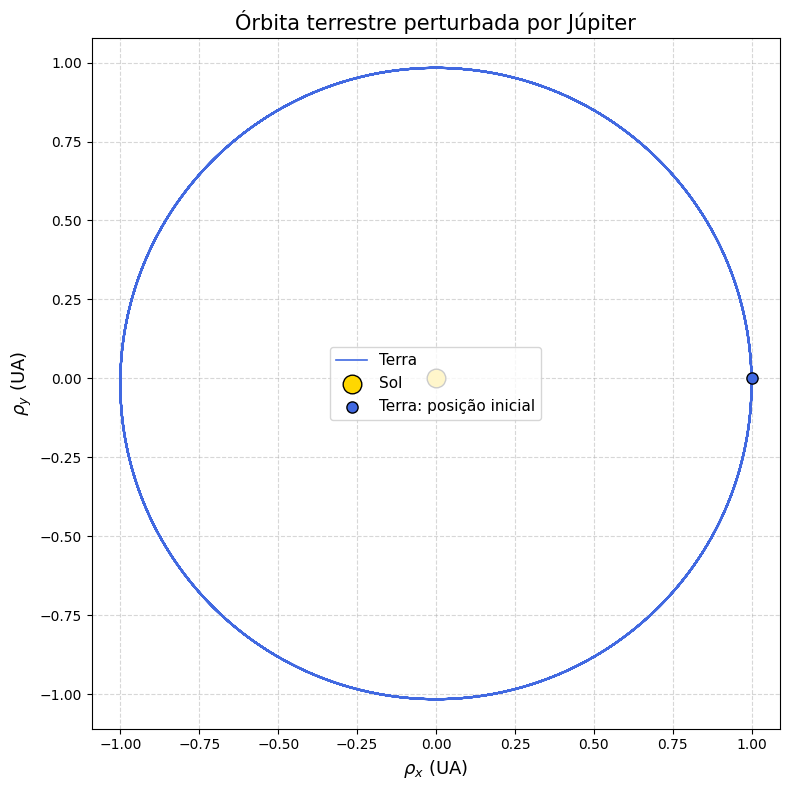
\includegraphics[width=0.9\textwidth]
    {tarefa-3b-grafico-1.png}
    \caption{Trajetória da Terra sob a perturbação gravitacional de Júpiter durante 30 anos.}
    \label{fig:orbita-terra-perturbada}
\end{figure}

Observa-se que a trajetória terrestre permanece aproximadamente circular, com raio próximo de uma unidade astronômica. 

A Figura \ref{fig:orbitas-terra-jupiter} apresenta simultaneamente as trajetórias da Terra e de Júpiter, permitindo visualizar a diferença entre suas escalas orbitais.

\begin{figure}[htbp]
    \centering
    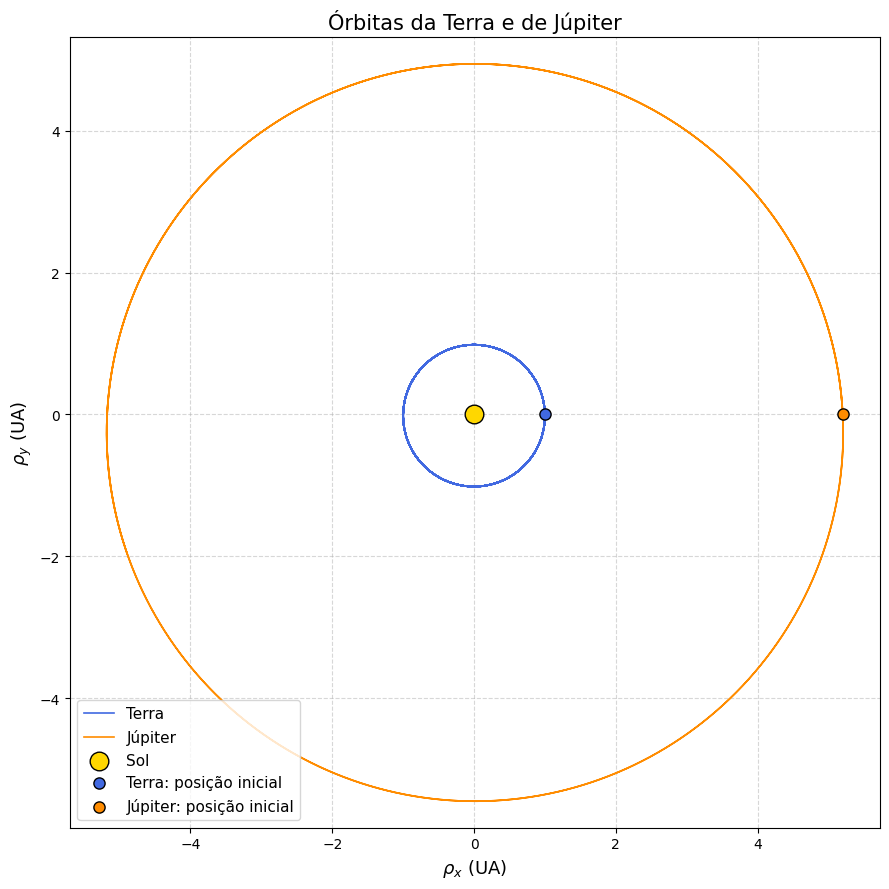
\includegraphics[width=0.9\textwidth]
    {tarefa-3b-grafico-2.png}
    \caption{Trajetórias da Terra e de Júpiter durante a integração numérica do sistema gravitacional acoplado.}
    \label{fig:orbitas-terra-jupiter}
\end{figure}

Verifica-se que Júpiter percorre uma trajetória muito mais extensa que a terrestre, devido à sua maior distância inicial ao Sol.

\paragraph{Distâncias entre posições terrestres em anos consecutivos}

Os valores calculados pelo programa para os 30 anos de integração estão apresentados na Tabela \ref{tab:desvios-anuais}. Todas as distâncias são expressas em unidades astronômicas (UA).

\begin{table}[htbp]
    \centering
    \caption{Distâncias entre posições terrestres correspondentes a anos consecutivos.}
    \label{tab:desvios-anuais}
    \scriptsize
    \begin{tabular}{r r r r}
        \hline
        Ano & Desvio (UA) & Ano & Desvio (UA) \\
        \hline
        1  & \texttt{1.7536132022175385E-003} & 16 & \texttt{7.0444035437735209E-004} \\
        2  & \texttt{1.5995115999186329E-003} & 17 & \texttt{3.2455523231811968E-004} \\
        3  & \texttt{1.2314218802369802E-003} & 18 & \texttt{1.6428934306687211E-004} \\
        4  & \texttt{7.5999747943334436E-004} & 19 & \texttt{3.6405368790220778E-004} \\
        5  & \texttt{3.6190779495137081E-004} & 20 & \texttt{6.6866792880871534E-004} \\
        6  & \texttt{1.6094346984125136E-004} & 21 & \texttt{9.9426330000452166E-004} \\
        7  & \texttt{3.3069531256403297E-004} & 22 & \texttt{1.3060585983169428E-003} \\
        8  & \texttt{6.3034890520414426E-004} & 23 & \texttt{1.5687231623164129E-003} \\
        9  & \texttt{9.5575095392355853E-004} & 24 & \texttt{1.7338489280834277E-003} \\
        10 & \texttt{1.2706367799341282E-003} & 25 & \texttt{1.7389567197169911E-003} \\
        11 & \texttt{1.5407304607945461E-003} & 26 & \texttt{1.5286374264481400E-003} \\
        12 & \texttt{1.7200461517546328E-003} & 27 & \texttt{1.1187308368715660E-003} \\
        13 & \texttt{1.7478991767230967E-003} & 28 & \texttt{6.5054180252889959E-004} \\
        14 & \texttt{1.5658179836294979E-003} & 29 & \texttt{2.9011880638620934E-004} \\
        15 & \texttt{1.1757791170910832E-003} & 30 & \texttt{1.7482663326268494E-004} \\
        \hline
    \end{tabular}
\end{table}

Os dados mostram que os desvios anuais não permanecem constantes ao longo da simulação. Inicialmente, ocorre uma diminuição progressiva da distância entre posições correspondentes a anos consecutivos, atingindo um mínimo no sexto ano. Posteriormente, os desvios voltam a aumentar, alcançando valores próximos de $1,75\times10^{-3}$ UA por volta do décimo terceiro ano.

A sequência apresenta, portanto, uma variação oscilatória, sem tendência monotônica de crescimento ou diminuição.

Assim, os resultados evidenciam que o movimento terrestre deixa de apresentar a repetição anual observada no modelo não perturbado.

\paragraph{Razão entre as distâncias máxima e mínima}

Para avaliar a extensão radial da trajetória terrestre, o programa calcula a razão entre as distâncias máxima e mínima ao Sol durante a integração:

\begin{equation}
    R=
    \frac{\rho_{\oplus,\max}}
    {\rho_{\oplus,\min}}.
\end{equation}

O resultado obtido numericamente foi

\begin{equation}
    \boxed{
    R_{\mathrm{num}}
    =
    1,0350209260862646
    }.
\end{equation}

Para estabelecer uma referência, considera-se a excentricidade original da órbita terrestre, $e_T=0,017$. Na ausência de perturbações, as distâncias mínima e máxima ao Sol para uma órbita elíptica são dadas por

\begin{equation}
    \rho_{\min}=a(1-e_T),
    \qquad
    \rho_{\max}=a(1+e_T).
\end{equation}

Consequentemente, a razão teórica esperada para a órbita não perturbada é

\begin{equation}
    R_{\mathrm{teórico}}
    =
    \frac{1+e_T}{1-e_T}
    =
    \frac{1+0,017}{1-0,017}.
\end{equation}

Numericamente,

\begin{equation}
    R_{\mathrm{teórico}}
    \approx1,034587995930824.
\end{equation}

Comparando os resultados, observa-se que a razão obtida numericamente é ligeiramente superior à previsão para a órbita não perturbada. A diferença absoluta é

\begin{equation}
    \Delta R=
    R_{\mathrm{num}}-R_{\mathrm{teórico}}
    \approx4,329301554406584\times10^{-4}.
\end{equation}

A diferença relativa, tomando o valor teórico como referência, é

\begin{equation}
    \eta=
    \frac{|R_{\mathrm{num}}-R_{\mathrm{teórico}}|}
    {R_{\mathrm{teórico}}}\times100\%
    \approx0,04185\%.
\end{equation}

Portanto, a razão entre as distâncias radiais máxima e mínima permanece bastante próxima daquela esperada para a órbita terrestre original, embora apresente um pequeno desvio decorrente da perturbação gravitacional de Júpiter.

\subsection{Item (c): Aumento da massa de Júpiter}

\subsubsection{Descrição do Problema}

Neste item, deve-se repetir a simulação do sistema Sol-Terra-Júpiter, multiplicando por 100 a massa de Júpiter em relação ao seu valor original.

O objetivo é construir, em um mesmo gráfico, as trajetórias da Terra e de Júpiter e investigar como o aumento da massa do planeta modifica a dinâmica orbital do sistema. A partir dos resultados, deve-se discutir a estabilidade do sistema solar.

% ORIENTAÇÕES À IA — ESTRATÉGIA DE SOLUÇÃO
% Consulte o código F77 e identifique precisamente como a massa de Júpiter é alterada por um fator 100, verificando se as demais massas, condições iniciais e parâmetros permanecem iguais.
% Explique como essa alteração modifica os termos de aceleração no sistema Sol-Terra-Júpiter e descreva o procedimento numérico usado para integrar os dois cenários, caso ambos sejam calculados.
% Informe o integrador, o passo temporal, o tempo total, as condições iniciais e como as trajetórias são gravadas e reunidas no gráfico comparativo.
% Verifique no código se o Sol permanece fixo ou se há tratamento dinâmico adicional; descreva a hipótese efetivamente implementada.
\subsubsection{Estratégia de Solução}

\paragraph{Alteração da massa de Júpiter}

A massa adimensional original de Júpiter é multiplicada por um fator 100, enquanto a massa da Terra permanece inalterada. Assim, os parâmetros utilizados são

\begin{equation}
    \mu_T=3,003\times10^{-6},
\end{equation}

\begin{equation}
    \mu_J=100\cdot9,545\times10^{-4}
    =9,545\times10^{-2}.
\end{equation}

Portanto, a massa de Júpiter passa a corresponder a aproximadamente $9,545\%$ da massa solar.

\paragraph{Análise da trajetória terrestre}

Da mesma forma, calcula-se a distância máxima e mínima da Terra ao Sol durante a integração.

A partir desses valores, determina-se a razão

\begin{equation}
    R=
    \frac{\rho_{\oplus,\max}}
    {\rho_{\oplus,\min}}.
\end{equation}

\begin{lstlisting}[
style=fortranstyle
]
      program tarefa3c
      ! O problema de três corpos: Sol, Terra e Júpiter com método de Verlet.
      ! Retorna ρ♁(τ) para um período de 30 anos simulando Júpiter 100 vezes mais massivo;
      ! Calcula ρ♁,max/ρ♁,min.
      ! Utiliza-se a 3a Lei de Kepler GM = 4pi^2 UA^3 ano^(-2).
      ! Grandezas adimensionais rho = r/UA, tau = 2pi*t/ano, v = v/(2pi*UA/ano).
      ! Toma-se o Sol como origem estática e Terra e Júpiter como corpos em órbita.

      implicit none

      character(30) filename
      real*8 taumax, dtau
      real*8 mu_terra, mu_jupiter
      real*8 e_original_terra, e_original_jupiter
      real*8 rx_terra(200000), ry_terra(200000), vx_terra, vy_terra
      real*8 rx_jupiter(200000), ry_jupiter(200000), 
     & vx_jupiter, vy_jupiter
      real*8 razao ! ρ♁,max/ρ♁,min
      real*8 pi
      parameter (pi = 3.14159265358979323d0)

      ! Massas adimensionais dos corpos
      mu_terra = 3.003d-6 ! massa da Terra
      mu_jupiter = 100.0d0 * 9.545d-4 ! massa de Júpiter

      e_original_terra = 0.017d0 ! excentricidade da órbita da Terra sem perturbação
      e_original_jupiter = 0.049d0 ! excentricidade da órbita de Júpiter sem perturbação

      ! Condições iniciais adimensionais
      ! Terra
      rx_terra(1) = 1.0d0 ! posição inicial no eixo x
      ry_terra(1) = 0.0d0 ! posição inicial no eixo y
      vx_terra = - e_original_terra / sqrt(rx_terra(1)) ! velocidade inicial no eixo x
      vy_terra = sqrt((1.0d0-e_original_terra**2)/rx_terra(1)) ! velocidade inicial no eixo y
      ! Júpiter
      rx_jupiter(1) = 5.2d0 ! posição inicial no eixo x
      ry_jupiter(1) = 0.0d0 ! posição inicial no eixo y
      vx_jupiter = - e_original_jupiter / sqrt(rx_jupiter(1)) ! velocidade inicial no eixo x
      vy_jupiter = sqrt((1.0d0-e_original_jupiter**2)/rx_jupiter(1)) ! velocidade inicial no eixo y

      ! Parâmetros da simulação
      taumax = 30.0d0 * 2.0d0 * pi ! 30 anos de simulação
      dtau = 2.0d0*pi/6284.0d0 ! passo de tempo adimensional
      ! Escolhemos esse dtau porque garante delta < 10^(-3)
      ! e discretiza o ano em 6284 passos inteiros

      ! Nome do arquivo de saída
      filename = 'tarefa-3c-saida-1.dat'

      ! Chamada da subrotina de simulação
      call simulacao_orbita(
     &     filename, rx_terra, ry_terra, vx_terra, vy_terra,
     &     rx_jupiter, ry_jupiter, vx_jupiter, vy_jupiter,
     &     mu_terra, mu_jupiter, dtau, taumax, razao)

      print *, 'Razao rho_max/rho_min = ', razao

      end program

      subroutine simulacao_orbita(
     &   filename, rx_terra, ry_terra, vx_terra, vy_terra,
     &   rx_jupiter, ry_jupiter, vx_jupiter, vy_jupiter,
     &   mu_terra, mu_jupiter, dtau, taumax, razao)
      ! Simulação via método de Verlet
      ! Retorna tau, rx, ry da Terra e de Júpiter, e calcula ρ♁,max/ρ♁,min
      implicit none
      character(30) filename
      real*8 rx_sol, ry_sol
      parameter (rx_sol = 0.0d0, ry_sol = 0.0d0) ! Sol na origem
      real*8 rx_terra(200000), ry_terra(200000), vx_terra, vy_terra
      real*8 rx_jupiter(200000), ry_jupiter(200000), 
     & vx_jupiter, vy_jupiter
      real*8 tau, dtau, taumax
      real*8 mu_jupiter, mu_terra
      real*8 aceleracao
      real*8 razao, rho_max, rho_min
      real*8 pi
      parameter (pi = 3.14159265358979323d0)
      integer*4 i, nsteps, nperyear
      
      ! Número de dtau's no ano
      nperyear = nint(2.0d0*pi/dtau)

      ! Número de passos da simulação
      nsteps = nint(taumax/dtau)

      ! Para o método de Verlet, precisamos de uma segunda posição inicial
      ! Calculamos os valores de rx(1), ry(1), vx(1), vy(1)
      ! por meio do método de Euler para calcular a posição do passo i=2
      open(10, file=filename) ! Posições e velocidades

      write(10,*) 0.0d0, rx_terra(1), ry_terra(1), 
     &   rx_jupiter(1), ry_jupiter(1)

      rx_terra(2) = rx_terra(1) + vx_terra*dtau
      ry_terra(2) = ry_terra(1) + vy_terra*dtau
      rx_jupiter(2) = rx_jupiter(1) + vx_jupiter*dtau
      ry_jupiter(2) = ry_jupiter(1) + vy_jupiter*dtau

      do i = 2, nsteps

        ! Atualização das posições da Terra
        rx_terra(i+1) = 2.0d0*rx_terra(i) - rx_terra(i-1)
     &       + aceleracao('x', rx_terra(i), ry_terra(i),
     &         rx_sol, ry_sol)*dtau**2
     &       + mu_jupiter*aceleracao('x',
     &         rx_terra(i), ry_terra(i),
     &         rx_jupiter(i), ry_jupiter(i))*dtau**2

        ry_terra(i+1) = 2.0d0*ry_terra(i) - ry_terra(i-1)
     &       + aceleracao('y', rx_terra(i), ry_terra(i),
     &         rx_sol, ry_sol)*dtau**2
     &       + mu_jupiter*aceleracao('y',
     &         rx_terra(i), ry_terra(i),
     &         rx_jupiter(i), ry_jupiter(i))*dtau**2

        ! Atualização das posições de Júpiter
        rx_jupiter(i+1) = 2.0d0*rx_jupiter(i)
     &       - rx_jupiter(i-1)
     &       + aceleracao('x', rx_jupiter(i), ry_jupiter(i),
     &         rx_sol, ry_sol)*dtau**2
     &       + mu_terra*aceleracao('x',
     &         rx_jupiter(i), ry_jupiter(i),
     &         rx_terra(i), ry_terra(i))*dtau**2

        ry_jupiter(i+1) = 2.0d0*ry_jupiter(i)
     &       - ry_jupiter(i-1)
     &       + aceleracao('y', rx_jupiter(i), ry_jupiter(i),
     &         rx_sol, ry_sol)*dtau**2
     &       + mu_terra*aceleracao('y',
     &         rx_jupiter(i), ry_jupiter(i),
     &         rx_terra(i), ry_terra(i))*dtau**2

        ! Escreve no arquivo de saída as posições da Terra e de Júpiter
        tau = (i-1)*dtau
        write(10,*) tau, rx_terra(i), ry_terra(i), 
     &   rx_jupiter(i), ry_jupiter(i)

      end do

      ! Cálculo da razão ρ♁,max/ρ♁,min
      rho_max = maxval(sqrt((rx_terra(1:nsteps) - rx_sol)**2 + 
     &     (ry_terra(1:nsteps) - ry_sol)**2))
      rho_min = minval(sqrt((rx_terra(1:nsteps) - rx_sol)**2 + 
     &     (ry_terra(1:nsteps) - ry_sol)**2))
      razao = rho_max / rho_min

      close(10)
      end subroutine


      function aceleracao(
     &   componente, rx_corpo_1, ry_corpo_1, rx_corpo_2, ry_corpo_2)
      ! Calcula a aceleração de um corpo devido à gravidade de outro corpo
      ! componente: 'x' para x, 'y' para y
      ! rx_corpo_1, ry_corpo_1: posição do corpo que sofre a aceleração
      ! rx_corpo_2, ry_corpo_2: posição do corpo que exerce a força gravitacional
      implicit none
      character*1 componente
      real*8 rx_corpo_1, ry_corpo_1, rx_corpo_2, ry_corpo_2
      real*8 aceleracao, r
      r = sqrt((rx_corpo_2 - rx_corpo_1)**2 + 
     & (ry_corpo_2 - ry_corpo_1)**2)
      if (componente .eq. 'x') then
        aceleracao = - (rx_corpo_1 - rx_corpo_2) / r**3
      else if (componente .eq. 'y') then
        aceleracao = - (ry_corpo_1 - ry_corpo_2) / r**3
      end if
      return
      end function
\end{lstlisting}


% ORIENTAÇÕES À IA — RESULTADOS OBTIDOS
% Apresente, no mesmo referencial e com escalas adequadas, as trajetórias da Terra e de Júpiter para a massa original e para a massa multiplicada por 100, conforme os dados disponíveis.
% Compare quantitativa e qualitativamente a alteração das órbitas, destacando mudanças no movimento terrestre e no movimento de Júpiter.
% Discuta o que os resultados permitem concluir sobre a estabilidade do sistema no intervalo simulado. Diferencie instabilidade observada nesse intervalo de uma afirmação sobre estabilidade de longo prazo do Sistema Solar real.
\subsubsection{Resultados Obtidos}

A Figura \ref{fig:terra-jupiter-massivo} apresenta a trajetória terrestre obtida durante os 30 anos de integração, considerando a massa de Júpiter multiplicada por 100.

\begin{figure}[htbp]
    \centering
    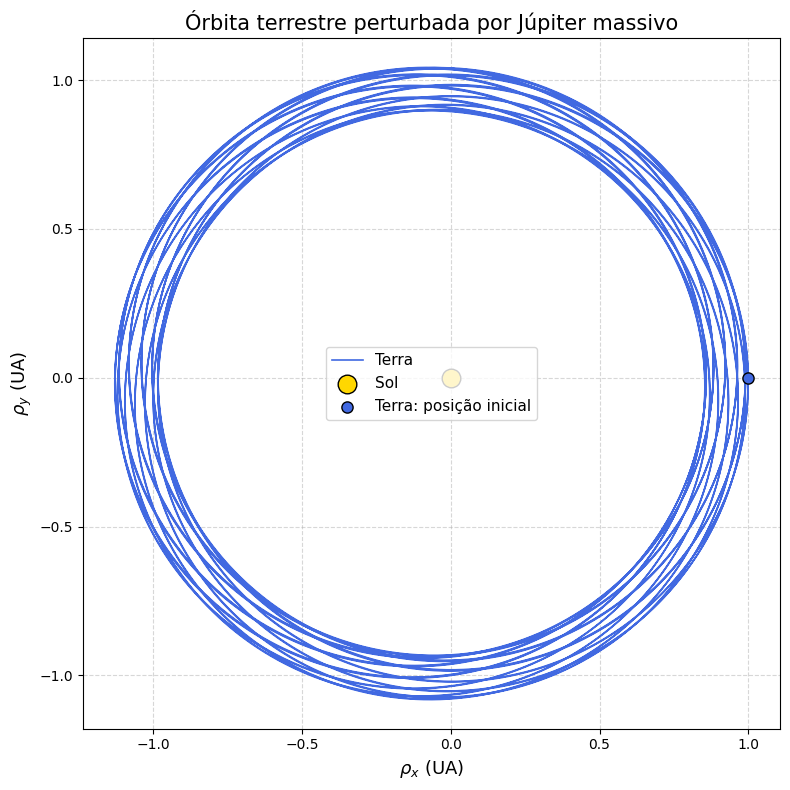
\includegraphics[width=0.9\textwidth]
    {tarefa-3c-grafico-1.png}
    \caption{Trajetória terrestre perturbada pela presença de Júpiter com massa multiplicada por 100.}
    \label{fig:terra-jupiter-massivo}
\end{figure}

Observa-se que a trajetória terrestre apresenta uma região de maior espessura em comparação com a órbita obtida no item anterior. Em vez de uma trajetória aproximadamente coincidente consigo mesma, observa-se um conjunto de curvas que se distribuem em torno da região orbital inicial.

Esse comportamento evidencia a intensificação das perturbações gravitacionais provocadas por Júpiter. Como sua massa foi aumentada por um fator 100, a força gravitacional desse planeta para a aceleração da Terra também é multiplicada por 100, para uma mesma configuração geométrica.

A Figura \ref{fig:orbitas-terra-jupiter-massivo} apresenta simultaneamente as trajetórias da Terra e de Júpiter, permitindo comparar os comportamentos orbitais dos dois planetas.

\begin{figure}[htbp]
    \centering
    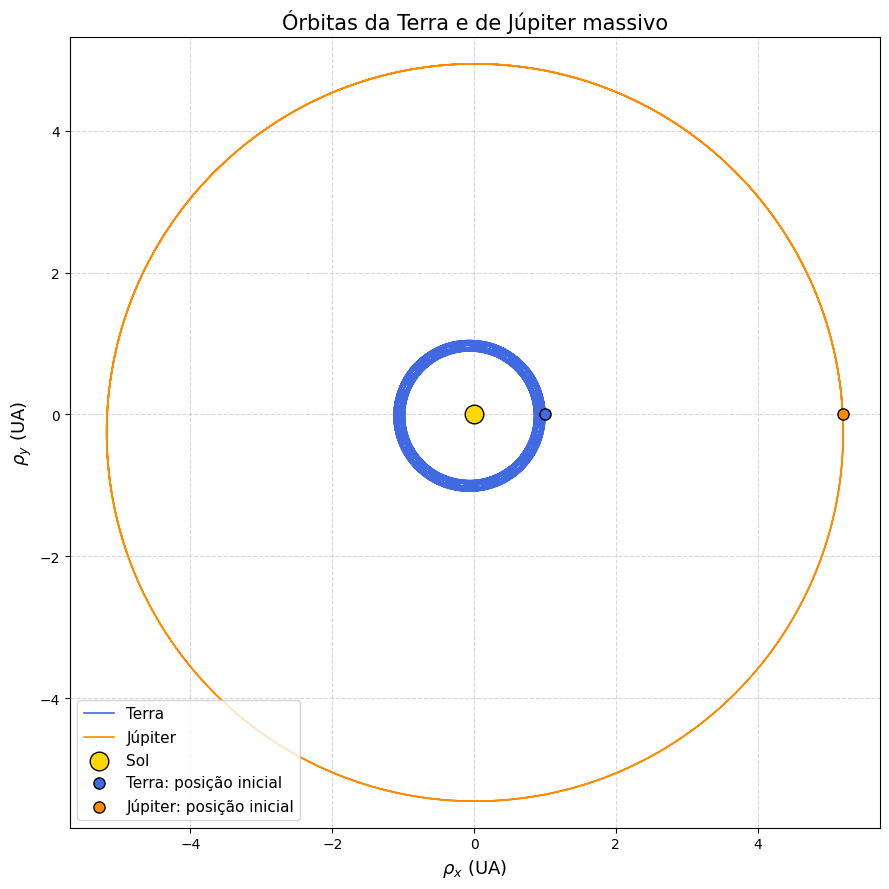
\includegraphics[width=0.9\textwidth]
    {tarefa-3c-grafico-2.png}
    \caption{Trajetórias da Terra e de Júpiter para uma massa de Júpiter multiplicada por 100.}
    \label{fig:orbitas-terra-jupiter-massivo}
\end{figure}

Verifica-se que Júpiter continua descrevendo uma trajetória aproximadamente circular, com raio próximo de $5,2$ UA. 

\paragraph{Razão entre as distâncias máxima e mínima}

Para quantificar a alteração da trajetória terrestre, calcula-se a razão entre as distâncias máxima e mínima ao Sol durante a integração:

\begin{equation}
    R=
    \frac{\rho_{\oplus,\max}}
    {\rho_{\oplus,\min}}.
\end{equation}

O resultado obtido numericamente foi

\begin{equation}
    \boxed{
    R_{\mathrm{num}}=1,3300142319721446
    }.
\end{equation}

Para comparação, no item anterior, em que Júpiter possuía sua massa original, foi obtido

\begin{equation}
    R_{\mathrm{original}}=1,0350209260862646.
\end{equation}

Portanto, o aumento da massa de Júpiter provoca um crescimento expressivo da razão entre as distâncias radiais extremas da Terra. A diferença relativa entre os dois resultados é

\begin{equation}
    \eta=
    \frac{R_{\mathrm{num}}-R_{\mathrm{original}}}
    {R_{\mathrm{original}}}\times100\%
    \approx28,50\%.
\end{equation}

Como referência adicional, para a órbita terrestre não perturbada, com excentricidade $e_T=0,017$, a razão esperada seria

\begin{equation}
    R_{\mathrm{teórico}}
    =
    \frac{1+e_T}{1-e_T}
    \approx1,03459.
\end{equation}

A diferença entre o resultado obtido com Júpiter massivo e essa referência é consideravelmente maior do que aquela observada no item anterior. Portanto, a presença de um Júpiter muito mais massivo modifica significativamente a extensão radial da trajetória terrestre.

\paragraph{Discussão sobre a estabilidade do sistema solar}

Os resultados demonstram como a órbita de um planeta pode ser instável na presença de outros corpos nos seus arredores. 

Nesse sentido, podemos considerar que a Terra se encontra em uma configuração orbital relativamente favorável: os planetas do Sistema Solar possuem massas pequenas em comparação à massa do Sol, de modo que suas influências gravitacionais mútuas são relativamente limitadas. Caso essas massas fossem significativamente maiores, as perturbações gravitacionais poderiam alterar consideravelmente as órbitas planetárias, modificando, por exemplo, os períodos de translação e, consequentemente, a duração dos anos.

\subsection{Item (d): Órbitas de asteroides e lacunas de Kirkwood}

\subsubsection{Descrição do Problema}

Neste item, considera-se a dinâmica de três asteroides localizados no cinturão de asteroides, entre Marte e Júpiter. São fornecidos os raios orbitais e as velocidades iniciais dos três objetos, enquanto Júpiter possui raio orbital de $5{,}2\,\mathrm{UA}$ e velocidade de $2{,}755\,\mathrm{UA/ano}$.

O objetivo é converter os dados fornecidos para as unidades adimensionais adotadas no projeto e simular as órbitas dos asteroides sob a ação gravitacional do Sol e de Júpiter, desprezando-se a influência dos asteroides sobre Júpiter. Por fim, deve-se discutir os resultados obtidos e sua relação com as lacunas de Kirkwood.

% ORIENTAÇÕES À IA — ESTRATÉGIA DE SOLUÇÃO
% Leia o código F77 e identifique os dados iniciais de cada asteroide e de Júpiter, bem como as conversões de UA, UA/ano e demais grandezas para as unidades adimensionais adotadas.
% Apresente as equações de aceleração dos asteroides sob a ação do Sol e de Júpiter. Explique como a posição de Júpiter é atualizada e confirme como o código despreza a reação gravitacional dos asteroides sobre Júpiter.
% Descreva o integrador, o passo temporal, o intervalo de simulação e os dados registrados para cada asteroide. Identifique como os parâmetros orbitais são representados nos arquivos de saída.
% Explique que aspecto da dinâmica ou que comparação com posições/resonâncias orbitais é usado para relacionar as simulações às lacunas de Kirkwood. Não pressuponha a implementação de cálculo de ressonância se ela não existir.
\subsubsection{Estratégia de Solução}

Neste item, considera-se a evolução orbital de três asteroides sob a ação gravitacional do Sol e de Júpiter. Diferentemente dos itens anteriores, os asteroides são tratados como corpos de massa desprezível, de modo que não exercem influência gravitacional sobre Júpiter nem interagem gravitacionalmente entre si.

\paragraph{Condições iniciais e conversão de unidades}

As posições iniciais dos asteroides são fornecidas em unidades astronômicas (UA), enquanto suas velocidades são fornecidas em UA/ano. Para utilizar as unidades adimensionais adotadas no projeto, empregam-se as relações

\begin{equation}
    \rho=\frac{r}{\mathrm{UA}},
    \qquad
    \upsilon=\frac{v}{2\pi\,\mathrm{UA}/\mathrm{ano}}.
\end{equation}

Assim, as velocidades fornecidas são divididas por $2\pi$. As condições iniciais utilizadas estão organizadas na Tabela \ref{tab:condicoes-asteroides}.

\begin{table}[htbp]
    \centering
    \caption{Condições iniciais dos asteroides e de Júpiter.}
    \label{tab:condicoes-asteroides}
    \begin{tabular}{c|c|c|c|c}
        \hline
        Corpo & $\rho_x(0)$ & $\rho_y(0)$ &
        $\upsilon_x(0)$ & $\upsilon_y(0)$ \\
        \hline
        Asteroide I & 3,000 & 0 & 0 & 0,577414 \\
        Asteroide II & 3,276 & 0 & 0 & 0,552427 \\
        Asteroide III & 3,700 & 0 & 0 & 0,519959 \\
        Júpiter & 5,200 & 0 & 0 & 0,438472 \\
        \hline
    \end{tabular}
\end{table}

A massa adimensional de Júpiter é

\begin{equation}
    \mu_J=9,545\times10^{-4}.
\end{equation}

\paragraph{Equações de movimento}

O Sol é mantido fixo na origem do sistema de coordenadas. Os três asteroides sofrem a atração gravitacional do Sol e de Júpiter. Portanto, para cada asteroide $k$, a aceleração adimensional é dada por

\begin{equation}
    \vec{a}_k=
    -\frac{\vec{\rho}_k}{|\vec{\rho}_k|^3}
    +
    \mu_J
    \frac{\vec{\rho}_J-\vec{\rho}_k}
    {|\vec{\rho}_J-\vec{\rho}_k|^3},
    \qquad k=I,II,III.
\end{equation}

O primeiro termo representa a atração gravitacional do Sol, enquanto o segundo corresponde à perturbação gravitacional provocada por Júpiter.

Por outro lado, como a influência dos asteroides sobre Júpiter é desprezada, sua aceleração é determinada exclusivamente pela atração gravitacional solar:

\begin{equation}
    \vec{a}_J=
    -\frac{\vec{\rho}_J}{|\vec{\rho}_J|^3}.
\end{equation}

Dessa maneira, Júpiter descreve uma órbita determinada pelo potencial gravitacional solar, enquanto sua posição é utilizada no cálculo das acelerações dos três asteroides.

\paragraph{Integração numérica}

A integração das equações de movimento é realizada pelo método de Verlet. Para cada corpo, a relação de recorrência utilizada é

\begin{equation}
    \vec{\rho}_{i+1}
    =
    2\vec{\rho}_i-\vec{\rho}_{i-1}
    +
    \vec{a}_i\Delta\tau^2.
\end{equation}

A segunda posição de cada corpo é inicializada por uma aproximação de Euler:

\begin{equation}
    \vec{\rho}_2=
    \vec{\rho}_1+\vec{\upsilon}_1\Delta\tau.
\end{equation}

Em cada iteração, são atualizadas as posições dos três asteroides utilizando a posição de Júpiter no mesmo índice temporal. Em seguida, atualiza-se a posição de Júpiter considerando apenas a atração solar.

A simulação é realizada durante 30 anos, com passo temporal adimensional constante:

\begin{equation}
    \tau_{\max}=60\pi,
    \qquad
    \Delta\tau=0,001.
\end{equation}

O número de passos é determinado por

\begin{equation}
    N=\operatorname{int}
    \left(\frac{\tau_{\max}}{\Delta\tau}\right)
    =188495.
\end{equation}

As posições dos corpos são armazenadas no arquivo \texttt{tarefa-3d-saida-1.dat}, contendo nove colunas: o tempo adimensional, as componentes cartesianas das posições dos três asteroides e as componentes cartesianas da posição de Júpiter.

\begin{lstlisting}[
style=fortranstyle
]
      program tarefa3d
      ! O problema de vários corpos: Sol, Júpiter e asteroides com método de Verlet.
      ! Retorna ρ(τ) de três asteroides no cinturão entre Marte e Júpiter
      ! Utiliza-se a 3a Lei de Kepler GM = 4pi^2 UA^3 ano^(-2).
      ! Grandezas adimensionais rho = r/UA, tau = 2pi*t/ano, v = v/(2pi*UA/ano).
      ! Toma-se o Sol como origem estática e outros corpos em órbita.

      implicit none

      character(30) filename
      real*8 taumax, dtau
      real*8 mu_jupiter
      real*8 rx_i(200000), ry_i(200000), vx_i, vy_i
      real*8 rx_ii(200000), ry_ii(200000), vx_ii, vy_ii
      real*8 rx_iii(200000), ry_iii(200000), vx_iii, vy_iii
      real*8 rx_jupiter(200000), ry_jupiter(200000), 
     & vx_jupiter, vy_jupiter
      real*8 pi
      parameter (pi = 3.14159265358979323d0)

      ! Massas adimensionais dos corpos
      mu_jupiter = 9.545d-4 ! massa de Júpiter

      ! Condições iniciais adimensionais
      ! Asteroides
      rx_i(1) = 3.000d0 ! posição inicial no eixo x
      rx_ii(1) = 3.276d0
      rx_iii(1) = 3.700d0
      ry_i(1) = 0.0d0 ! posição inicial no eixo y
      ry_ii(1) = 0.0d0
      ry_iii(1) = 0.0d0
      vx_i = 0.0d0 ! velocidade inicial no eixo x
      vx_ii = 0.0d0
      vx_iii = 0.0d0
      vy_i = 3.628d0 / (2.0d0 * pi) ! velocidade inicial no eixo y
      vy_ii = 3.471d0 / (2.0d0 * pi)
      vy_iii = 3.267d0 / (2.0d0 * pi)
      ! Júpiter
      rx_jupiter(1) = 5.2d0 ! posição inicial no eixo x
      ry_jupiter(1) = 0.0d0 ! posição inicial no eixo y
      vx_jupiter = 0.0d0 ! velocidade inicial no eixo x
      vy_jupiter = 2.755 / (2.0d0 * pi) ! velocidade inicial no eixo y (órbita circular)

      ! Parâmetros da simulação
      taumax = 30.0d0 * 2.0d0 * pi ! 30 anos de simulação
      dtau = 0.001 ! passo de tempo adimensional

      ! Nome do arquivo de saída
      filename = 'tarefa-3d-saida-1.dat'

      ! Chamada da subrotina de simulação
      call simulacao_orbita(
     &   filename,
     &   rx_i, ry_i, vx_i, vy_i,
     &   rx_ii, ry_ii, vx_ii, vy_ii,
     &   rx_iii, ry_iii, vx_iii, vy_iii,
     &   rx_jupiter, ry_jupiter, vx_jupiter, vy_jupiter,
     &   mu_jupiter, dtau, taumax)

      end program

      subroutine simulacao_orbita(
     &   filename,
     &   rx_i, ry_i, vx_i, vy_i,
     &   rx_ii, ry_ii, vx_ii, vy_ii,
     &   rx_iii, ry_iii, vx_iii, vy_iii,
     &   rx_jupiter, ry_jupiter, vx_jupiter, vy_jupiter,
     &   mu_jupiter, dtau, taumax)
      ! Simulação via método de Verlet
      ! Considera apenas a interação gravitacional do Sol e de Júpiter sobre os asteroides
      ! Retorna tau, rx, ry dos asteroides e de Júpiter
      implicit none
      character(30) filename
      real*8 rx_sol, ry_sol
      parameter (rx_sol = 0.0d0, ry_sol = 0.0d0)
      real*8 rx_i(200000), ry_i(200000), vx_i, vy_i
      real*8 rx_ii(200000), ry_ii(200000), vx_ii, vy_ii
      real*8 rx_iii(200000), ry_iii(200000), vx_iii, vy_iii
      real*8 rx_jupiter(200000), ry_jupiter(200000)
      real*8 vx_jupiter, vy_jupiter
      real*8 tau, dtau, taumax
      real*8 mu_jupiter
      real*8 aceleracao
      real*8 pi
      parameter (pi = 3.14159265358979323d0)
      integer*4 i, nsteps, nperyear

      ! Número de dtau's no ano
      nperyear = nint(2.0d0*pi/dtau)

      ! Número de passos da simulação
      nsteps = nint(taumax/dtau)

      ! Inicialização das posições para o método de Verlet
      open(10, file=filename)

      write(10,*) 0.0d0,
     &   rx_i(1), ry_i(1),
     &   rx_ii(1), ry_ii(1),
     &   rx_iii(1), ry_iii(1),
     &   rx_jupiter(1), ry_jupiter(1)

      rx_i(2) = rx_i(1) + vx_i*dtau
      ry_i(2) = ry_i(1) + vy_i*dtau

      rx_ii(2) = rx_ii(1) + vx_ii*dtau
      ry_ii(2) = ry_ii(1) + vy_ii*dtau

      rx_iii(2) = rx_iii(1) + vx_iii*dtau
      ry_iii(2) = ry_iii(1) + vy_iii*dtau

      rx_jupiter(2) = rx_jupiter(1) + vx_jupiter*dtau
      ry_jupiter(2) = ry_jupiter(1) + vy_jupiter*dtau

      do i = 2, nsteps

        ! Atualização das posições do Asteroide I
        rx_i(i+1) = 2.0d0*rx_i(i) - rx_i(i-1)
     &       + aceleracao('x', rx_i(i), ry_i(i),
     &         rx_sol, ry_sol)*dtau**2
     &       + mu_jupiter*aceleracao('x',
     &         rx_i(i), ry_i(i),
     &         rx_jupiter(i), ry_jupiter(i))*dtau**2

        ry_i(i+1) = 2.0d0*ry_i(i) - ry_i(i-1)
     &       + aceleracao('y', rx_i(i), ry_i(i),
     &         rx_sol, ry_sol)*dtau**2
     &       + mu_jupiter*aceleracao('y',
     &         rx_i(i), ry_i(i),
     &         rx_jupiter(i), ry_jupiter(i))*dtau**2

        ! Atualização das posições do Asteroide II
        rx_ii(i+1) = 2.0d0*rx_ii(i) - rx_ii(i-1)
     &       + aceleracao('x', rx_ii(i), ry_ii(i),
     &         rx_sol, ry_sol)*dtau**2
     &       + mu_jupiter*aceleracao('x',
     &         rx_ii(i), ry_ii(i),
     &         rx_jupiter(i), ry_jupiter(i))*dtau**2

        ry_ii(i+1) = 2.0d0*ry_ii(i) - ry_ii(i-1)
     &       + aceleracao('y', rx_ii(i), ry_ii(i),
     &         rx_sol, ry_sol)*dtau**2
     &       + mu_jupiter*aceleracao('y',
     &         rx_ii(i), ry_ii(i),
     &         rx_jupiter(i), ry_jupiter(i))*dtau**2

        ! Atualização das posições do Asteroide III
        rx_iii(i+1) = 2.0d0*rx_iii(i) - rx_iii(i-1)
     &       + aceleracao('x', rx_iii(i), ry_iii(i),
     &         rx_sol, ry_sol)*dtau**2
     &       + mu_jupiter*aceleracao('x',
     &         rx_iii(i), ry_iii(i),
     &         rx_jupiter(i), ry_jupiter(i))*dtau**2

        ry_iii(i+1) = 2.0d0*ry_iii(i) - ry_iii(i-1)
     &       + aceleracao('y', rx_iii(i), ry_iii(i),
     &         rx_sol, ry_sol)*dtau**2
     &       + mu_jupiter*aceleracao('y',
     &         rx_iii(i), ry_iii(i),
     &         rx_jupiter(i), ry_jupiter(i))*dtau**2

        ! Atualização das posições de Júpiter
        ! Júpiter sofre apenas a atração gravitacional do Sol
        rx_jupiter(i+1) = 2.0d0*rx_jupiter(i)
     &       - rx_jupiter(i-1)
     &       + aceleracao('x', rx_jupiter(i), ry_jupiter(i),
     &         rx_sol, ry_sol)*dtau**2

        ry_jupiter(i+1) = 2.0d0*ry_jupiter(i)
     &       - ry_jupiter(i-1)
     &       + aceleracao('y', rx_jupiter(i), ry_jupiter(i),
     &         rx_sol, ry_sol)*dtau**2

        ! Escreve no arquivo de saída as posições dos corpos
        tau = (i-1)*dtau
        write(10,*) tau,
     &       rx_i(i), ry_i(i),
     &       rx_ii(i), ry_ii(i),
     &       rx_iii(i), ry_iii(i),
     &       rx_jupiter(i), ry_jupiter(i)

      end do

      close(10)
      end subroutine


      function aceleracao(
     &   componente, rx_corpo_1, ry_corpo_1, rx_corpo_2, ry_corpo_2)
      ! Calcula a aceleração de um corpo devido à gravidade de outro corpo
      ! componente: 'x' para x, 'y' para y
      ! rx_corpo_1, ry_corpo_1: posição do corpo que sofre a aceleração
      ! rx_corpo_2, ry_corpo_2: posição do corpo que exerce a força gravitacional
      implicit none
      character*1 componente
      real*8 rx_corpo_1, ry_corpo_1, rx_corpo_2, ry_corpo_2
      real*8 aceleracao, r
      r = sqrt((rx_corpo_2 - rx_corpo_1)**2 + 
     & (ry_corpo_2 - ry_corpo_1)**2)
      if (componente .eq. 'x') then
        aceleracao = - (rx_corpo_1 - rx_corpo_2) / r**3
      else if (componente .eq. 'y') then
        aceleracao = - (ry_corpo_1 - ry_corpo_2) / r**3
      end if
      return
      end function
\end{lstlisting}


% ORIENTAÇÕES À IA — RESULTADOS OBTIDOS
% Apresente as trajetórias dos três asteroides e de Júpiter, identificando cada objeto e mantendo uma escala que permita comparar suas órbitas.
% Descreva as diferenças observadas entre os asteroides, como variações orbitais, aproximações, perturbações ou eventual comportamento de escape, somente quando sustentadas pelos resultados.
% Relacione os comportamentos às lacunas de Kirkwood com cuidado: indique quais evidências da simulação são compatíveis com perturbações ou ressonâncias com Júpiter e quais conclusões não podem ser estabelecidas apenas pelos gráficos.
\subsubsection{Resultados Obtidos}

A Figura \ref{fig:orbitas-asteroides} apresenta as trajetórias dos três asteroides e de Júpiter durante os 30 anos de simulação.

\begin{figure}[htbp]
    \centering
    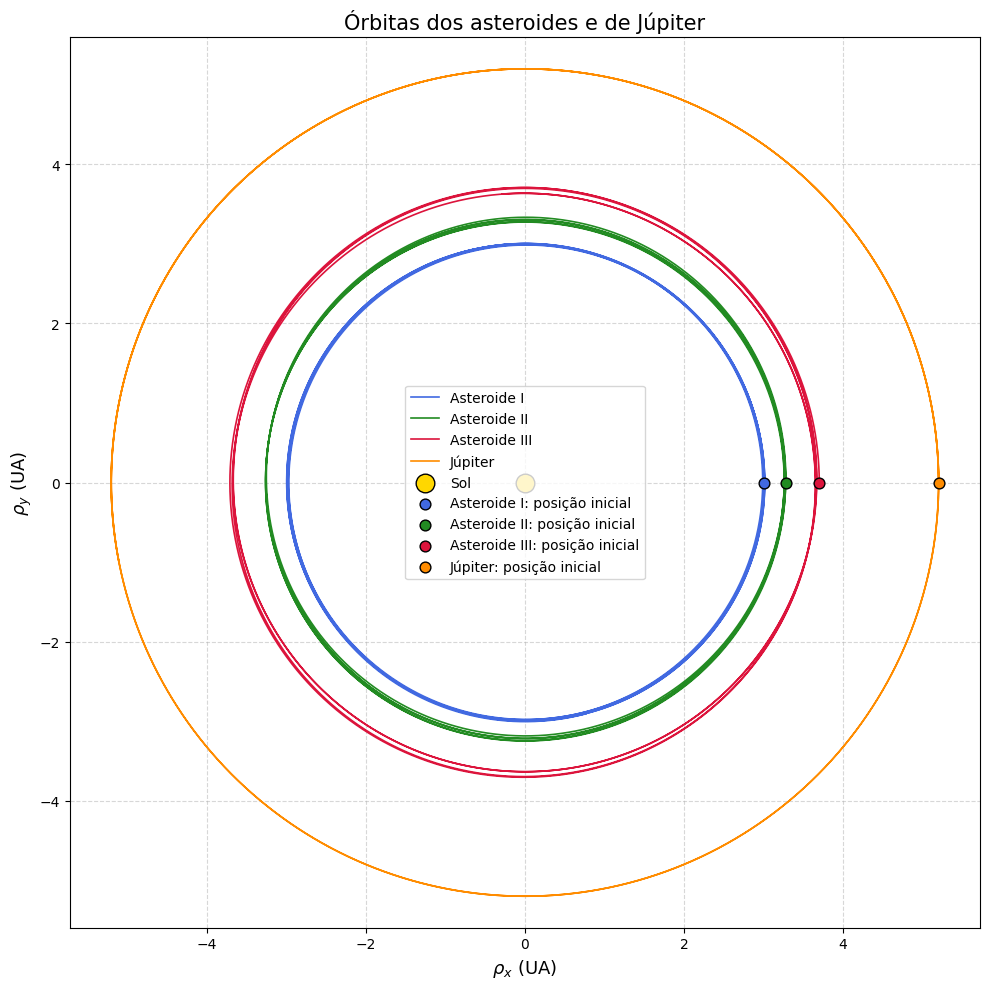
\includegraphics[width=0.9\textwidth]
    {tarefa-3d-grafico-1.png}
    \caption{Trajetórias dos três asteroides e de Júpiter durante o intervalo de integração.}
    \label{fig:orbitas-asteroides}
\end{figure}

Observa-se que os três asteroides permanecem em regiões orbitais distintas, com trajetórias aproximadamente circulares, mas apresentam pequenas variações em relação às órbitas circulares que seriam obtidas na ausência de Júpiter.

Essas variações decorrem da interação gravitacional com o planeta gigante. Como os asteroides possuem diferentes posições e velocidades iniciais, suas configurações orbitais em relação a Júpiter também são distintas, resultando em perturbações diferentes ao longo da integração.

Júpiter, por sua vez, apresenta uma trajetória aproximadamente circular de raio $5,2$ UA, conforme esperado pelo modelo adotado. Isso ocorre porque sua aceleração é calculada exclusivamente a partir da atração gravitacional solar, sem considerar a reação dos asteroides.

\paragraph{Relação com as lacunas de Kirkwood}

As lacunas de Kirkwood são regiões do cinturão de asteroides caracterizadas por uma menor concentração de objetos, associadas principalmente a ressonâncias orbitais com Júpiter.

Uma ressonância orbital ocorre quando os períodos de revolução de dois corpos apresentam uma razão próxima de números inteiros. Nessas configurações, perturbações gravitacionais periódicas podem se acumular e modificar significativamente a evolução orbital dos corpos envolvidos.

Para investigar a relação entre as condições iniciais utilizadas e essas ressonâncias, podemos estimar os períodos orbitais keplerianos dos asteroides e de Júpiter. Na aproximação de um problema de dois corpos, em unidades adimensionais, vale

\begin{equation}
    T=2\pi a^{3/2},
\end{equation}

em que $a$ é o semieixo maior da órbita em unidades astronômicas.

Considerando as órbitas inicialmente circulares, os períodos aproximados são apresentados na Tabela \ref{tab:periodos-asteroides}.

\begin{table}[htbp]
    \centering
    \caption{Períodos orbitais keplerianos aproximados dos corpos.}
    \label{tab:periodos-asteroides}
    \begin{tabular}{c|c|c}
        \hline
        Corpo & $a$ (UA) & $T$ (anos) \\
        \hline
        Asteroide I & 3,000 & 5,196 \\
        Asteroide II & 3,276 & 5,930 \\
        Asteroide III & 3,700 & 7,117 \\
        Júpiter & 5,200 & 11,858 \\
        \hline
    \end{tabular}
\end{table}

Um resultado particularmente interessante é o do Asteroide II. Seu período orbital é aproximadamente metade do período de Júpiter, caracterizando uma configuração próxima da ressonância 2:1:

\begin{equation}
    \frac{T_J}{T_{II}}\approx2.
\end{equation}

Essa ressonância está associada a uma das principais lacunas de Kirkwood, localizada aproximadamente em $3,28$ UA.

O Asteroide I, por sua vez, encontra-se relativamente próximo da região associada à ressonância 7:3, enquanto o Asteroide III não está inicialmente próximo de uma das principais ressonâncias responsáveis pelas lacunas mais conhecidas.

\subsection{Item (e): Simulação conjunta dos planetas (opcional)}

\subsubsection{Descrição do Problema}

Neste item opcional, propõe-se colocar todos os planetas do Sistema Solar no mesmo plano e realizar simulações numéricas de suas interações gravitacionais. O objetivo é observar a evolução dinâmica do sistema e investigar qualitativamente os comportamentos orbitais resultantes.

% ORIENTAÇÕES À IA — ESTRATÉGIA DE SOLUÇÃO
% Examine o código F77 e identifique quais planetas são incluídos, suas massas e condições iniciais, bem como o referencial e as hipóteses do modelo.
% Descreva as equações de movimento implementadas e esclareça explicitamente quais interações gravitacionais são consideradas: planeta-Sol, planeta-planeta e, se aplicável, movimento do próprio Sol. Não suponha que o modelo seja heliocêntrico com Sol fixo ou que inclua todas as interações sem conferir o código.
% Explique como o método numérico calcula as acelerações do sistema de muitos corpos, como atualiza simultaneamente as posições e velocidades e como trata as distâncias entre partículas.
% Informe passo temporal, duração, unidades, critérios de inicialização e arquivos de saída, além das simplificações adotadas.
\subsubsection{Estratégia de Solução}

\paragraph{Unidades e massas dos planetas}

São utilizadas as unidades adimensionais adotadas nos itens anteriores:

\begin{equation}
    \rho=\frac{r}{\mathrm{UA}},
    \qquad
    \tau=\frac{2\pi t}{\mathrm{ano}},
    \qquad
    \upsilon=\frac{v}{2\pi\mathrm{UA}/\mathrm{ano}}.
\end{equation}

As massas dos planetas são expressas em unidades da massa solar, conforme os valores definidos no código:

\begin{table}[htbp]
    \centering
    \caption{Massas adimensionais dos planetas utilizadas na simulação.}
    \label{tab:massas-planetas}
    \begin{tabular}{c c}
        \hline
        Planeta & $\mu=M_{\mathrm{planeta}}/M_{\odot}$ \\
        \hline
        Mercúrio & $1,6601\times10^{-7}$ \\
        Vênus & $2,4478\times10^{-6}$ \\
        Terra & $3,0035\times10^{-6}$ \\
        Marte & $3,2272\times10^{-7}$ \\
        Júpiter & $9,5479\times10^{-4}$ \\
        Saturno & $2,8589\times10^{-4}$ \\
        Urano & $4,3662\times10^{-5}$ \\
        Netuno & $5,1514\times10^{-5}$ \\
        \hline
    \end{tabular}
\end{table}

\paragraph{Condições iniciais}

Todos os planetas são inicialmente posicionados sobre o eixo positivo $x$, com velocidades exclusivamente tangenciais. As posições iniciais são determinadas pelos respectivos raios orbitais, conforme a Tabela \ref{tab:posicoes-planetas}.

\begin{table}[htbp]
    \centering
    \caption{Posições iniciais dos planetas em unidades astronômicas.}
    \label{tab:posicoes-planetas}
    \begin{tabular}{c c}
        \hline
        Planeta & $\rho_x(0)$ (UA) \\
        \hline
        Mercúrio & $0,3871$ \\
        Vênus & $0,7233$ \\
        Terra & $1,0000$ \\
        Marte & $1,5237$ \\
        Júpiter & $5,2026$ \\
        Saturno & $9,5549$ \\
        Urano & $19,2184$ \\
        Netuno & $30,1104$ \\
        \hline
    \end{tabular}
\end{table}

As condições iniciais de velocidade são dadas por

\begin{equation}
    \upsilon_{x,0}=0,
    \qquad
    \upsilon_{y,0}=\frac{1}{\sqrt{\rho_x(0)}}.
\end{equation}

Essa escolha corresponde à velocidade orbital circular kepleriana na ausência das perturbações dos demais planetas.

\paragraph{Modelo gravitacional e integração numérica}

É utilizado o método de Verlet para integração numérica. As interações gravitacionais consideradas relevam ambas as forças entre os planetas quanto a força com o Sol. 
Assim, o modelo é realista no sentido da quantidade de interações, mesmo que as interações entre os planetas seja pequena frente à força causada pelo Sol.
\paragraph{Parâmetros da simulação e armazenamento}

O intervalo de integração e o passo temporal são definidos por

\begin{equation}
    \tau_{\max}=30\cdot2\pi=60\pi,
\end{equation}

\begin{equation}
    \Delta\tau=0,001.
\end{equation}

A simulação corresponde, portanto, a 30 anos nas unidades temporais adotadas.

Os resultados são destinados ao arquivo \texttt{tarefa-3e-saida-1.dat}. Conforme os comentários do programa, são armazenadas as posições dos oito planetas ao longo do tempo, permitindo representar suas trajetórias no mesmo referencial.

A análise dos resultados é realizada por meio da representação gráfica das órbitas, observando-se suas escalas, formas e extensões durante o intervalo simulado.

\begin{lstlisting}[
style=fortranstyle
]

      program tarefa3e
      ! O problema de varios corpos: sistema solar com metodo de Verlet.
      ! Retorna rho(tau) dos oito planetas.
      ! Utiliza-se a 3a Lei de Kepler GM_sol = 4pi^2 UA^3 ano^(-2).
      ! Grandezas adimensionais rho = r/UA, tau = 2pi*t/ano,
      ! v = v/(2pi*UA/ano).
      ! Toma-se o Sol como origem estatica.

      implicit none

      character(30) filename
      real*8 taumax, dtau

      real*8 mu_mercurio, mu_venus, mu_terra, mu_marte
      real*8 mu_jupiter, mu_saturno, mu_urano, mu_netuno

      real*8 rx_mercurio(200000), ry_mercurio(200000)
      real*8 vx_mercurio, vy_mercurio

      real*8 rx_venus(200000), ry_venus(200000)
      real*8 vx_venus, vy_venus

      real*8 rx_terra(200000), ry_terra(200000)
      real*8 vx_terra, vy_terra

      real*8 rx_marte(200000), ry_marte(200000)
      real*8 vx_marte, vy_marte

      real*8 rx_jupiter(200000), ry_jupiter(200000)
      real*8 vx_jupiter, vy_jupiter

      real*8 rx_saturno(200000), ry_saturno(200000)
      real*8 vx_saturno, vy_saturno

      real*8 rx_urano(200000), ry_urano(200000)
      real*8 vx_urano, vy_urano

      real*8 rx_netuno(200000), ry_netuno(200000)
      real*8 vx_netuno, vy_netuno

      real*8 pi
      parameter (pi = 3.14159265358979323d0)

      ! Massas adimensionais dos planetas: M_planeta/M_sol
      mu_mercurio = 1.6601d-7
      mu_venus = 2.4478d-6
      mu_terra = 3.0035d-6
      mu_marte = 3.2272d-7
      mu_jupiter = 9.5479d-4
      mu_saturno = 2.8589d-4
      mu_urano = 4.3662d-5
      mu_netuno = 5.1514d-5

      ! Condicoes iniciais adimensionais
      ! Todos os planetas com orbitas inicialmente circulares
      ! e alinhados sobre o eixo x.

      ! Mercurio
      rx_mercurio(1) = 0.3871d0
      ry_mercurio(1) = 0.0d0
      vx_mercurio = 0.0d0
      vy_mercurio = 1.0d0/sqrt(rx_mercurio(1))

      ! Venus
      rx_venus(1) = 0.7233d0
      ry_venus(1) = 0.0d0
      vx_venus = 0.0d0
      vy_venus = 1.0d0/sqrt(rx_venus(1))

      ! Terra
      rx_terra(1) = 1.0000d0
      ry_terra(1) = 0.0d0
      vx_terra = 0.0d0
      vy_terra = 1.0d0/sqrt(rx_terra(1))

      ! Marte
      rx_marte(1) = 1.5237d0
      ry_marte(1) = 0.0d0
      vx_marte = 0.0d0
      vy_marte = 1.0d0/sqrt(rx_marte(1))

      ! Jupiter
      rx_jupiter(1) = 5.2026d0
      ry_jupiter(1) = 0.0d0
      vx_jupiter = 0.0d0
      vy_jupiter = 1.0d0/sqrt(rx_jupiter(1))

      ! Saturno
      rx_saturno(1) = 9.5549d0
      ry_saturno(1) = 0.0d0
      vx_saturno = 0.0d0
      vy_saturno = 1.0d0/sqrt(rx_saturno(1))

      ! Urano
      rx_urano(1) = 19.2184d0
      ry_urano(1) = 0.0d0
      vx_urano = 0.0d0
      vy_urano = 1.0d0/sqrt(rx_urano(1))

      ! Netuno
      rx_netuno(1) = 30.1104d0
      ry_netuno(1) = 0.0d0
      vx_netuno = 0.0d0
      vy_netuno = 1.0d0/sqrt(rx_netuno(1))

      ! Parametros da simulacao
      taumax = 30.0d0*2.0d0*pi
      dtau = 0.001d0

      ! Nome do arquivo de saida
      filename = 'tarefa-3e-saida-1.dat'

      ! Chamada da subrotina de simulacao
      call simulacao_orbita(
     &   filename,
     &   rx_mercurio, ry_mercurio, vx_mercurio, vy_mercurio,
     &   rx_venus, ry_venus, vx_venus, vy_venus,
     &   rx_terra, ry_terra, vx_terra, vy_terra,
     &   rx_marte, ry_marte, vx_marte, vy_marte,
     &   rx_jupiter, ry_jupiter, vx_jupiter, vy_jupiter,
     &   rx_saturno, ry_saturno, vx_saturno, vy_saturno,
     &   rx_urano, ry_urano, vx_urano, vy_urano,
     &   rx_netuno, ry_netuno, vx_netuno, vy_netuno,
     &   mu_mercurio, mu_venus, mu_terra, mu_marte,
     &   mu_jupiter, mu_saturno, mu_urano, mu_netuno,
     &   dtau, taumax)

      end program

      ...

\end{lstlisting}


% ORIENTAÇÕES À IA — RESULTADOS OBTIDOS
% Apresente as trajetórias dos planetas efetivamente incluídos, com legenda, unidades e escalas que permitam interpretá-las.
% Descreva os comportamentos orbitais qualitativos observados e eventuais perturbações, aproximações ou mudanças de configuração que estejam visíveis ou quantificadas.
% Discuta as limitações do modelo e do tempo de integração. Não generalize resultados de uma simulação curta para a estabilidade de longo prazo do Sistema Solar.
\subsubsection{Resultados Obtidos}

A Figura \ref{fig:orbitas-sistema-solar} apresenta as trajetórias dos oito planetas durante os 30 anos de integração, considerando o Sol fixo na origem.

\begin{figure}[htbp]
    \centering
    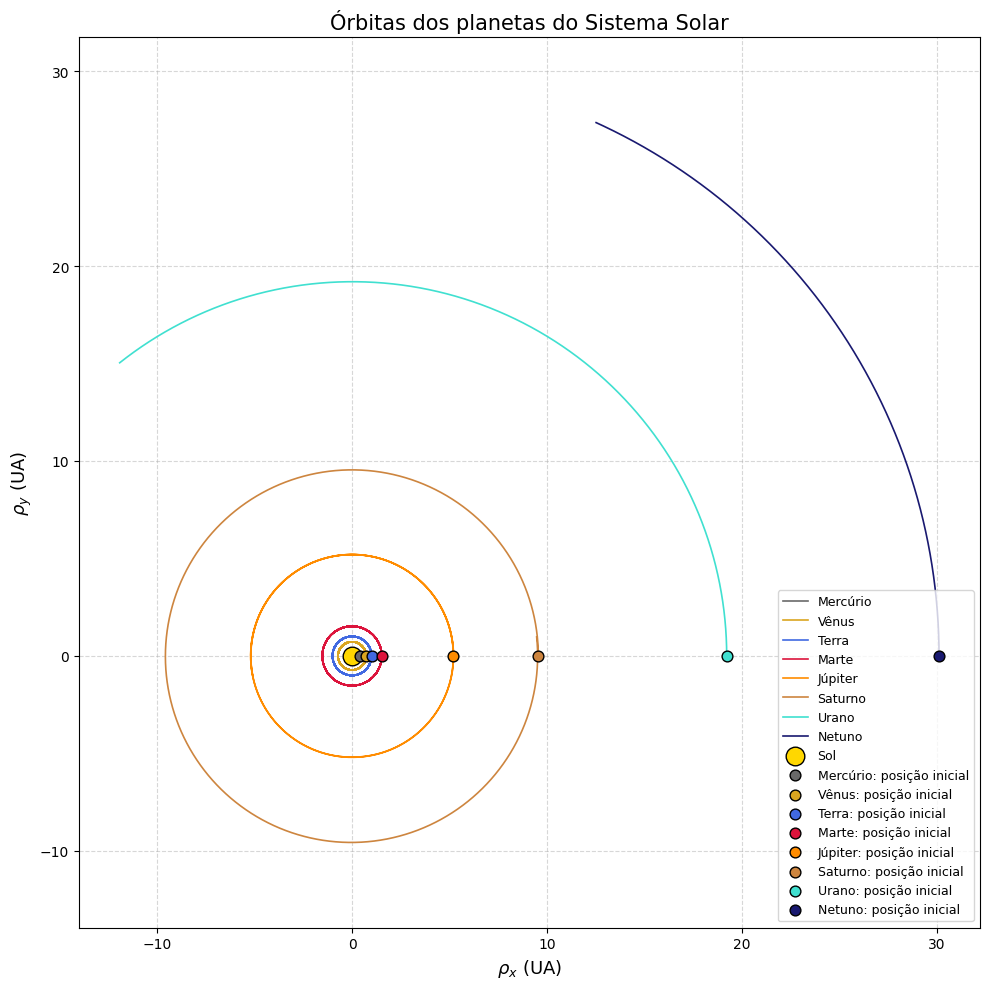
\includegraphics[width=0.9\textwidth]
    {tarefa-3e-grafico-1.png}
    \caption{Trajetórias dos oito planetas do Sistema Solar durante o intervalo de 30 anos.}
    \label{fig:orbitas-sistema-solar}
\end{figure}

Observa-se uma grande diferença entre as escalas orbitais dos planetas. Mercúrio, Vênus, Terra e Marte apresentam trajetórias concentradas nas proximidades do Sol, enquanto Júpiter e Saturno descrevem órbitas consideravelmente maiores. Urano e Netuno apresentam apenas arcos de suas trajetórias no intervalo representado.

Em particular, as trajetórias de Urano e Netuno não completam uma revolução no intervalo considerado. Isso decorre de seus períodos de revolução muito superiores à duração da simulação.
Pela Terceira Lei de Kepler, já era esperado que órbitas de maior raio tivessem período maior.

A representação gráfica permite observar que as órbitas dos planetas interiores ficam bastante próximas entre si quando comparadas à escala necessária para representar Netuno. Por esse motivo, as trajetórias de Mercúrio, Vênus, Terra e Marte aparecem concentradas em uma pequena região próxima à origem.

\subsection{Item (f): Coordenadas planetárias vistas da Terra e cálculo de eclipses (desafio opcional)}

\subsubsection{Descrição do Problema}

Neste desafio opcional, deve-se desenvolver um programa capaz de calcular as coordenadas aparentes dos planetas ao longo do ano, utilizando a Terra como referencial de observação. Adicionalmente, propõe-se implementar um programa para identificar e calcular eclipses lunares e solares.

% ORIENTAÇÕES À IA — ESTRATÉGIA DE SOLUÇÃO
% Leia os códigos F77 deste desafio e separe a rotina de cálculo das coordenadas aparentes da rotina de identificação de eclipses, se forem programas distintos.
% Para as coordenadas aparentes, explique como as posições heliocêntricas dos planetas e da Terra são combinadas para obter vetores geocêntricos. Descreva as coordenadas angulares calculadas, a convenção angular e o tratamento do referencial, conforme o código.
% Para os eclipses, identifique os corpos considerados, os vetores usados e o critério geométrico implementado para reconhecer alinhamento. Se o programa adotar alinhamento perfeito dos vetores, diga isso explicitamente e explique como a ordem dos corpos distingue eclipse solar de lunar.
% Descreva como o instante do evento é localizado e impresso, incluindo a resolução temporal e a eventual exigência de igualdade/alinhamento numérico. Não afirme que o programa calcula penumbra, umbra, diâmetros aparentes ou condições de eclipse parcial se esses efeitos não estiverem implementados.
% Verifique como as coordenadas heliocêntricas da Terra são preservadas no arquivo de saída e utilizadas na conversão para o referencial terrestre, se esse procedimento estiver presente no código.
\subsubsection{Estratégia de Solução}

\paragraph{Modelo gravitacional}

As interações gravitacionais entre os oito planetas são consideradas, assim como a atração gravitacional exercida pelo Sol sobre todos eles. A Lua também sofre a atração gravitacional do Sol e dos oito planetas. Entretanto, sua influência gravitacional sobre os demais corpos é desprezada.

A posição inicial da Lua é estabelecida a partir da posição inicial da Terra, considerando a distância média entre os dois corpos:

\begin{equation}
    d_{TL}=
    \frac{384400}{149597870,7}
    \approx0,002570\ \mathrm{UA}.
\end{equation}

Consequentemente,

\begin{equation}
    \vec{\rho}_{L,0}
    =
    \vec{\rho}_{T,0}+(d_{TL},0).
\end{equation}

A velocidade inicial da Lua possui a mesma componente radial da Terra e uma componente tangencial adicional, determinada pela aproximação de órbita circular do sistema Terra--Lua:

\begin{equation}
    \upsilon_{L,x,0}=\upsilon_{T,x,0},
\end{equation}

\begin{equation}
    \upsilon_{L,y,0}
    =
    \upsilon_{T,y,0}
    +
    \sqrt{\frac{\mu_T+\mu_L}{d_{TL}}}.
\end{equation}

Assim, a velocidade relativa inicial da Lua em relação à Terra é calculada considerando a massa dos dois corpos, embora a influência gravitacional da Lua sobre a Terra não seja posteriormente incluída na integração.

\paragraph{Integração numérica}

A evolução temporal dos planetas e da Lua é realizada pelo método de Verlet no referencial do Sol

\paragraph{Transformação para o referencial terrestre}

Para representar os corpos a partir da Terra, utiliza-se uma translação da origem para a posição terrestre.

Assim, o vetor posição de um planeta $j$ em relação à Terra é

\begin{equation}
    \vec{\rho}_{j/T}
    =
    \vec{\rho}_j-\vec{\rho}_T.
\end{equation}

Em componentes cartesianas,

\begin{equation}
    \rho_{j/T,x}=\rho_{j,x}-\rho_{T,x},
    \qquad
    \rho_{j/T,y}=\rho_{j,y}-\rho_{T,y}.
\end{equation}

Para a Lua, aplica-se a mesma transformação:

\begin{equation}
    \vec{\rho}_{L/T}
    =
    \vec{\rho}_L-\vec{\rho}_T.
\end{equation}

A Terra passa, portanto, a ocupar a origem do sistema de coordenadas, enquanto os demais corpos são representados por suas posições relativas a ela. Essa transformação consiste em uma translação, sem rotação dos eixos coordenados.

O arquivo de saída contém 21 colunas: tempo adimensional, duas coordenadas para cada um dos sete planetas distintos da Terra, duas coordenadas nulas para a Terra, duas coordenadas relativas da Lua e duas coordenadas adicionais da posição heliocêntrica da Terra, utilizadas no procedimento de representação do Sol.

\paragraph{Detecção de eclipses}

A identificação dos eclipses é realizada a partir das posições relativas do Sol, da Terra e da Lua. Para isso, definem-se os vetores com origem na Terra:

\begin{equation}
    \vec{s}=(-\rho_{T,x},-\rho_{T,y}),
\end{equation}

\begin{equation}
    \vec{m}=
    (\rho_{L,x}-\rho_{T,x},
    \rho_{L,y}-\rho_{T,y}).
\end{equation}

O primeiro vetor representa a direção da Terra para o Sol, enquanto o segundo representa a direção da Terra para a Lua.

As respectivas distâncias são calculadas por

\begin{equation}
    d_S=|\vec{s}|,
    \qquad
    d_L=|\vec{m}|.
\end{equation}

Para verificar o alinhamento, calculam-se o produto escalar e o produto vetorial bidimensional entre os vetores:

\begin{equation}
    P=\vec{s}\cdot\vec{m}
    =s_xm_x+s_ym_y,
\end{equation}

\begin{equation}
    Q=s_xm_y-s_ym_x.
\end{equation}

O critério de alinhamento adotado pelo programa é

\begin{equation}
    |Q|\leq\epsilon d_Sd_L,
\end{equation}

em que a tolerância utilizada é

\begin{equation}
    \epsilon=0,02.
\end{equation}

Como $|Q|/(d_Sd_L)$ corresponde ao módulo do seno do ângulo entre os vetores, esse critério admite desvios angulares em relação ao alinhamento perfeito. Próximo às configurações paralela e antiparalela, a tolerância corresponde aproximadamente a $0,020$ radianos, ou $1,15^\circ$.

Após a verificação do alinhamento, o tipo de eclipse é determinado pelo sinal do produto escalar e pela comparação das distâncias.

Um eclipse solar é identificado quando os vetores apresentam o mesmo sentido, isto é, quando $P>0$, e a Lua está mais próxima da Terra do que o Sol:

\begin{equation}
    P>0
    \qquad\text{e}\qquad
    d_L<d_S.
\end{equation}

Um eclipse lunar é identificado quando os vetores apresentam sentidos opostos:

\begin{equation}
    P<0.
\end{equation}

\paragraph{Registro dos eventos e parâmetros da simulação}

Os eclipses são identificados a cada iteração. Para evitar a impressão repetida de um mesmo evento enquanto a condição de alinhamento permanece satisfeita, o programa compara o tipo de eclipse atual com o tipo registrado na iteração anterior.

Um evento somente é impresso quando o tipo atual é diferente de zero e diferente do tipo anterior. Assim, são registrados os inícios das ocorrências identificadas pelo critério geométrico.

O instante do evento é convertido para anos por

\begin{equation}
    t_{\mathrm{anos}}=\frac{\tau}{2\pi}.
\end{equation}

O mês correspondente é determinado pela expressão

\begin{equation}
    M=
    \operatorname{int}
    \left(
    12\frac{\tau}{2\pi}
    \right)+1.
\end{equation}

A integração é realizada durante um ano terrestre:

\begin{equation}
    \tau_{\max}=2\pi,
\end{equation}

com passo temporal constante

\begin{equation}
    \Delta\tau=0,001.
\end{equation}

As posições relativas dos corpos são armazenadas no arquivo \texttt{tarefa-3f-saida-1.dat}, enquanto os instantes e os tipos de eclipse identificados são apresentados no terminal.

\begin{lstlisting}[
style=fortranstyle
]

      program tarefa3f
      ! O problema de varios corpos: sistema solar com metodo de Verlet conforme visto pela Terra.
      ! Retorna rho(tau) dos oito planetas no referencial da Terra.
      ! Utiliza-se a 3a Lei de Kepler GM_sol = 4pi^2 UA^3 ano^(-2).
      ! Grandezas adimensionais rho = r/UA, tau = 2pi*t/ano,
      ! v = v/(2pi*UA/ano).
      ! Toma-se o Sol como origem estatica.

      implicit none

      character(30) filename
      real*8 taumax, dtau

      real*8 mu_mercurio, mu_venus, mu_terra, mu_marte
      real*8 mu_jupiter, mu_saturno, mu_urano, mu_netuno

      real*8 rx_mercurio(200000), ry_mercurio(200000)
      real*8 vx_mercurio, vy_mercurio

      real*8 rx_venus(200000), ry_venus(200000)
      real*8 vx_venus, vy_venus

      real*8 rx_terra(200000), ry_terra(200000)
      real*8 vx_terra, vy_terra

      real*8 rx_marte(200000), ry_marte(200000)
      real*8 vx_marte, vy_marte

      real*8 rx_jupiter(200000), ry_jupiter(200000)
      real*8 vx_jupiter, vy_jupiter

      real*8 rx_saturno(200000), ry_saturno(200000)
      real*8 vx_saturno, vy_saturno

      real*8 rx_urano(200000), ry_urano(200000)
      real*8 vx_urano, vy_urano

      real*8 rx_netuno(200000), ry_netuno(200000)
      real*8 vx_netuno, vy_netuno

      real*8 mu_lua
      real*8 rx_lua(200000), ry_lua(200000)
      real*8 vx_lua, vy_lua

      real*8 pi
      parameter (pi = 3.14159265358979323d0)

      ! Massas adimensionais dos planetas: M_planeta/M_sol
      mu_mercurio = 1.6601d-7
      mu_venus = 2.4478d-6
      mu_terra = 3.0035d-6
      mu_marte = 3.2272d-7
      mu_jupiter = 9.5479d-4
      mu_saturno = 2.8589d-4
      mu_urano = 4.3662d-5
      mu_netuno = 5.1514d-5
      mu_lua = 3.694d-8

      ! Condicoes iniciais adimensionais
      ! Todos os planetas com orbitas inicialmente circulares
      ! e alinhados sobre o eixo x.

      ! Mercurio
      rx_mercurio(1) = 0.3871d0
      ry_mercurio(1) = 0.0d0
      vx_mercurio = 0.0d0
      vy_mercurio = 1.0d0/sqrt(rx_mercurio(1))

      ! Venus
      rx_venus(1) = 0.7233d0
      ry_venus(1) = 0.0d0
      vx_venus = 0.0d0
      vy_venus = 1.0d0/sqrt(rx_venus(1))

      ! Terra
      rx_terra(1) = 1.0000d0
      ry_terra(1) = 0.0d0
      vx_terra = 0.0d0
      vy_terra = 1.0d0/sqrt(rx_terra(1))

      ! Marte
      rx_marte(1) = 1.5237d0
      ry_marte(1) = 0.0d0
      vx_marte = 0.0d0
      vy_marte = 1.0d0/sqrt(rx_marte(1))

      ! Jupiter
      rx_jupiter(1) = 5.2026d0
      ry_jupiter(1) = 0.0d0
      vx_jupiter = 0.0d0
      vy_jupiter = 1.0d0/sqrt(rx_jupiter(1))

      ! Saturno
      rx_saturno(1) = 9.5549d0
      ry_saturno(1) = 0.0d0
      vx_saturno = 0.0d0
      vy_saturno = 1.0d0/sqrt(rx_saturno(1))

      ! Urano
      rx_urano(1) = 19.2184d0
      ry_urano(1) = 0.0d0
      vx_urano = 0.0d0
      vy_urano = 1.0d0/sqrt(rx_urano(1))

      ! Netuno
      rx_netuno(1) = 30.1104d0
      ry_netuno(1) = 0.0d0
      vx_netuno = 0.0d0
      vy_netuno = 1.0d0/sqrt(rx_netuno(1))

      ! Lua
      rx_lua(1) = rx_terra(1) + 384400.0d0/149597870.7d0
      ry_lua(1) = ry_terra(1)
      vx_lua = vx_terra
      vy_lua = vy_terra +
     &   sqrt((mu_terra+mu_lua)/
     &   (384400.0d0/149597870.7d0)) ! calculada via aproximação de órbita circular do sistema Terra–Lua

      ! Parametros da simulacao
      taumax = 1.0d0 * 2.0d0*pi ! 1 ano terrestre
      dtau = 0.001d0

      ! Nome do arquivo de saida
      filename = 'tarefa-3f-saida-1.dat'

      ! Chamada da subrotina de simulacao
      call simulacao_orbita(
     &   filename,
     &   rx_mercurio, ry_mercurio, vx_mercurio, vy_mercurio,
     &   rx_venus, ry_venus, vx_venus, vy_venus,
     &   rx_terra, ry_terra, vx_terra, vy_terra,
     &   rx_marte, ry_marte, vx_marte, vy_marte,
     &   rx_jupiter, ry_jupiter, vx_jupiter, vy_jupiter,
     &   rx_saturno, ry_saturno, vx_saturno, vy_saturno,
     &   rx_urano, ry_urano, vx_urano, vy_urano,
     &   rx_netuno, ry_netuno, vx_netuno, vy_netuno,
     &   mu_mercurio, mu_venus, mu_terra, mu_marte,
     &   mu_jupiter, mu_saturno, mu_urano, mu_netuno, mu_lua,
     &   rx_lua, ry_lua, vx_lua, vy_lua,
     &   dtau, taumax)

      end program

      ...

\end{lstlisting}


% ORIENTAÇÕES À IA — RESULTADOS OBTIDOS
% Apresente os gráficos ou tabelas das coordenadas aparentes dos planetas vistos da Terra, identificando os corpos, o intervalo temporal e as unidades angulares.
% Descreva os eclipses identificados, informando instante e tipo (solar ou lunar) conforme a saída do programa. Não acrescente eventos que não constem dos resultados.
% Explique as limitações do critério geométrico adotado. Em particular, se o código exige alinhamento perfeito, esclareça que se trata de um critério idealizado e não de uma modelagem completa das condições observacionais de eclipses reais.
% Comente consistência, resolução temporal e eventuais limitações numéricas dos resultados, sem inferir precisão maior que a permitida pelo passo da simulação.
\subsubsection{Resultados Obtidos}

A Figura \ref{fig:coordenadas-terra} apresenta a representação do Sistema Solar no referencial terrestre durante um ano, juntamente com a trajetória da Lua em relação à Terra.

\begin{figure}[htbp]
    \centering
    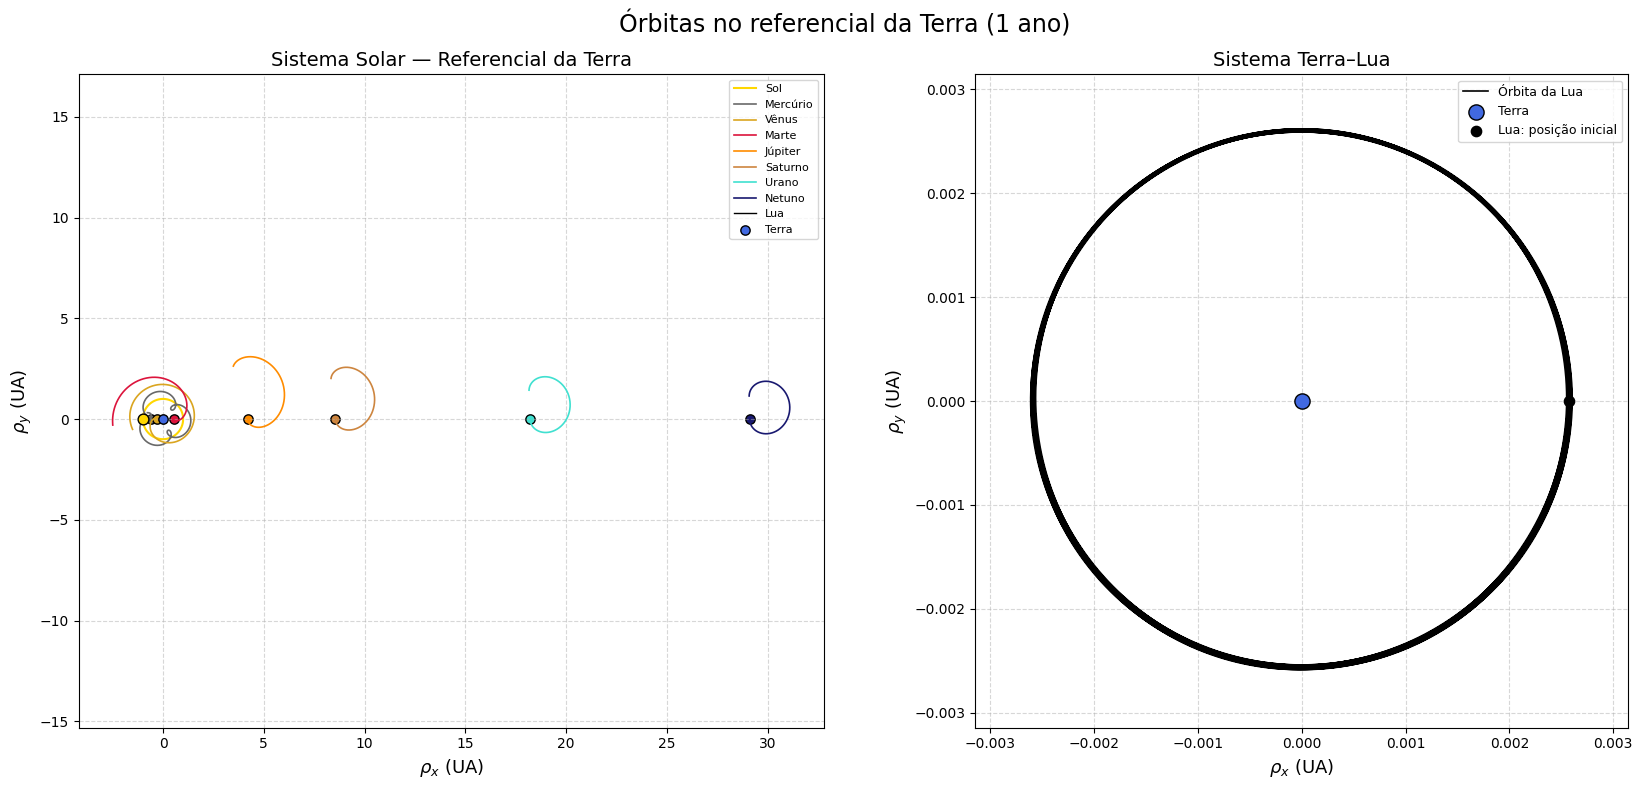
\includegraphics[width=\textwidth]
    {tarefa-3f-grafico-1.png}
    \caption{Trajetórias dos planetas e da Lua no referencial terrestre durante um ano. O painel da direita apresenta em maior escala a órbita relativa da Lua em torno da Terra.}
    \label{fig:coordenadas-terra}
\end{figure}

No painel esquerdo, observa-se o movimento dos planetas em relação à Terra, posicionada na origem do referencial. O Sol também apresenta movimento aparente, pois sua posição relativa é determinada pela translação da origem para a posição terrestre.

É interessante notar a presença dos movimentos que inspiraram a hipótese dos epiciclos no modelo ptolomaico. Esses movimentos são oriundos das forças de inércia presentes no referencial não-inercial da Terra.
Galileu utilizou esse comportamento inercial para defender o seu modelo heliocêntrico.

No painel direito, apresenta-se a órbita da Lua em relação à Terra. Observa-se uma trajetória aproximadamente circular, com raio próximo de $0,00257$ UA, compatível com a distância inicial de 384400 km utilizada na construção das condições iniciais.

\paragraph{Eclipses solares e lunares}

Durante o intervalo de um ano, o programa identificou 12 eclipses solares e 13 eclipses lunares. Os eventos são classificados a partir do alinhamento aproximado entre os vetores Terra--Sol e Terra--Lua.

Os resultados para os eclipses solares estão apresentados na Tabela \ref{tab:eclipses-solares}.

\begin{table}[htbp]
    \centering
    \caption{Eclipses solares identificados durante a simulação.}
    \label{tab:eclipses-solares}
    \scriptsize
    \begin{tabular}{c c c}
        \hline
        Mês & Tempo $\tau$ & Tempo (anos) \\
        \hline
        1 & \texttt{0.25900000000000001} & \texttt{4.1221130260800896E-002} \\
        2 & \texttt{0.77500000000000002} & \texttt{0.12334508089621890} \\
        3 & \texttt{1.2909999999999999} & \texttt{0.20546903153163687} \\
        4 & \texttt{1.8060000000000000} & \texttt{0.28743382722396299} \\
        5 & \texttt{2.3220000000000001} & \texttt{0.36955777785938099} \\
        6 & \texttt{2.8380000000000001} & \texttt{0.45168172849479898} \\
        7 & \texttt{3.3540000000000001} & \texttt{0.53380567913021704} \\
        8 & \texttt{3.8710000000000000} & \texttt{0.61608878470872686} \\
        9 & \texttt{4.3870000000000005} & \texttt{0.69821273534414496} \\
        10 & \texttt{4.9039999999999999} & \texttt{0.78049584092265478} \\
        11 & \texttt{5.4210000000000003} & \texttt{0.86277894650116471} \\
        12 & \texttt{5.9370000000000003} & \texttt{0.94490289713658271} \\
        \hline
    \end{tabular}
\end{table}

Os eclipses lunares identificados estão apresentados na Tabela \ref{tab:eclipses-lunares}.

\begin{table}[htbp]
    \centering
    \caption{Eclipses lunares identificados durante a simulação.}
    \label{tab:eclipses-lunares}
    \scriptsize
    \begin{tabular}{c c c}
        \hline
        Mês & Tempo $\tau$ & Tempo (anos) \\
        \hline
        1 & \texttt{1.0000000000000000E-003} & \texttt{1.5915494309189535E-004} \\
        2 & \texttt{0.51500000000000001} & \texttt{8.1964795692326106E-002} \\
        3 & \texttt{1.0320000000000000} & \texttt{0.16424790127083599} \\
        4 & \texttt{1.5489999999999999} & \texttt{0.24653100684934587} \\
        5 & \texttt{2.0649999999999999} & \texttt{0.32865495748476387} \\
        6 & \texttt{2.5819999999999999} & \texttt{0.41093806306327374} \\
        7 & \texttt{3.0979999999999999} & \texttt{0.49306201369869174} \\
        8 & \texttt{3.6150000000000002} & \texttt{0.57534511927720167} \\
        9 & \texttt{4.1310000000000002} & \texttt{0.65746906991261966} \\
        10 & \texttt{4.6470000000000002} & \texttt{0.73959302054803766} \\
        11 & \texttt{5.1619999999999999} & \texttt{0.82155781624036373} \\
        12 & \texttt{5.6779999999999999} & \texttt{0.90368176687578172} \\
        13 & \texttt{6.1940000000000000} & \texttt{0.98580571751119972} \\
        \hline
    \end{tabular}
\end{table}

Observa-se que os eclipses solares e lunares se alternam ao longo do intervalo de integração. Os eventos ocorrem aproximadamente a cada meio mês, sendo identificados sucessivamente os dois tipos de configuração geométrica.

\vspace{0.5cm}
\hrule
\vspace{0.5cm}

\section{Problema 4: Coreografias celestes}

\subsection{Item (a): Solução de Lagrange -- órbitas circulares}

\subsubsection{Descrição do Problema}

Neste item, considera-se um sistema de três partículas de massas iguais $M$, que interagem gravitacionalmente e se movimentam em torno do centro de massa do sistema. O objetivo é estudar uma solução particular do problema de três corpos, conhecida como solução de Lagrange, na qual as partículas descrevem órbitas circulares mantendo, em todos os instantes, as mesmas distâncias entre si e formando um triângulo equilátero.

São fornecidas as posições e velocidades iniciais das três partículas, em unidades adimensionais, com velocidade inicial determinada por $\upsilon_0=3^{-1/4}$. Deve-se verificar numericamente se as órbitas permanecem circulares e se as distâncias entre as partículas se mantêm iguais ao longo da simulação.

% ORIENTAÇÕES À IA — ESTRATÉGIA DE SOLUÇÃO
% Leia o código F77 e descreva como as três partículas de massas iguais são inicializadas, incluindo posições, velocidades e o valor υ₀ = 3-¹/⁴.
% Apresente as equações do problema gravitacional de três corpos implementadas no programa e explique como cada partícula sofre a ação das outras duas. Identifique o tratamento do centro de massa e o integrador numérico.
% Explique como são calculadas as distâncias par a par e, se implementado, o raio de cada partícula em relação ao centro de massa. Informe passo temporal, duração da simulação e variáveis gravadas.
% Descreva como os dados permitem verificar a configuração triangular equilátera e o caráter circular das trajetórias, sem atribuir ao código verificações que sejam feitas apenas visualmente.

\subsubsection{Estratégia de Solução}

\paragraph{Condições iniciais}

As posições iniciais são escolhidas de modo que as três partículas formem um triângulo equilátero de lado $\sqrt{3}$, centrado na origem:

\begin{equation}
    \vec{\rho}_{I,0}=(1,0),
\end{equation}

\begin{equation}
    \vec{\rho}_{II,0}=
    \left(-\frac{1}{2},\frac{\sqrt{3}}{2}\right),
\end{equation}

\begin{equation}
    \vec{\rho}_{III,0}=
    \left(-\frac{1}{2},-\frac{\sqrt{3}}{2}\right).
\end{equation}

As distâncias iniciais entre as partículas são, portanto,

\begin{equation}
    d_{I,II}=d_{II,III}=d_{III,I}=\sqrt{3}.
\end{equation}

As velocidades iniciais são determinadas a partir da constante

\begin{equation}
    \upsilon_0=3^{-1/4}.
\end{equation}

Consequentemente, suas componentes são

\begin{equation}
    \vec{\upsilon}_{I,0}=(0,\upsilon_0),
\end{equation}

\begin{equation}
    \vec{\upsilon}_{II,0}=
    \left(
    -\frac{\sqrt{3}}{2}\upsilon_0,
    -\frac{1}{2}\upsilon_0
    \right),
\end{equation}

\begin{equation}
    \vec{\upsilon}_{III,0}=
    \left(
    \frac{\sqrt{3}}{2}\upsilon_0,
    -\frac{1}{2}\upsilon_0
    \right).
\end{equation}

Observa-se que as três partículas possuem velocidades de mesmo módulo, tangentes às respectivas circunferências centradas na origem.

Além disso, devido à simetria das condições iniciais e à igualdade das massas, o centro de massa é inicialmente localizado na origem:

\begin{equation}
    \vec{R}_{CM}(0)
    =
    \frac{
    \vec{\rho}_{I,0}
    +\vec{\rho}_{II,0}
    +\vec{\rho}_{III,0}
    }{3}
    =\vec{0}.
\end{equation}

A soma das velocidades iniciais também é nula, de modo que o centro de massa permanece em repouso no referencial adotado.

\paragraph{Equações de movimento}

Cada partícula sofre a atração gravitacional das outras duas. Para uma partícula $i$, sua aceleração adimensional é dada por

\begin{equation}
    \vec{a}_i=
    \sum_{\substack{j=I,II,III\\j\neq i}}
    \mu_j
    \frac{\vec{\rho}_j-\vec{\rho}_i}
    {|\vec{\rho}_j-\vec{\rho}_i|^3}.
\end{equation}

Como todas as massas adimensionais são unitárias, as equações específicas são

\begin{equation}
    \vec{a}_I=
    \frac{\vec{\rho}_{II}-\vec{\rho}_I}
    {|\vec{\rho}_{II}-\vec{\rho}_I|^3}
    +
    \frac{\vec{\rho}_{III}-\vec{\rho}_I}
    {|\vec{\rho}_{III}-\vec{\rho}_I|^3},
\end{equation}

\begin{equation}
    \vec{a}_{II}=
    \frac{\vec{\rho}_I-\vec{\rho}_{II}}
    {|\vec{\rho}_I-\vec{\rho}_{II}|^3}
    +
    \frac{\vec{\rho}_{III}-\vec{\rho}_{II}}
    {|\vec{\rho}_{III}-\vec{\rho}_{II}|^3},
\end{equation}

\begin{equation}
    \vec{a}_{III}=
    \frac{\vec{\rho}_I-\vec{\rho}_{III}}
    {|\vec{\rho}_I-\vec{\rho}_{III}|^3}
    +
    \frac{\vec{\rho}_{II}-\vec{\rho}_{III}}
    {|\vec{\rho}_{II}-\vec{\rho}_{III}|^3}.
\end{equation}

Essas expressões são implementadas pela subrotina \texttt{derivadas}, que calcula as derivadas das posições e velocidades das três partículas. A função auxiliar \texttt{aceleracao} determina cada contribuição gravitacional a partir das posições relativas dos corpos.

\paragraph{Integração pelo método de Runge-Kutta de quarta ordem}

A integração numérica é realizada pelo método de Runge-Kutta de quarta ordem (RK4), e não pelo método de Verlet.

Para isso, o programa organiza as variáveis do sistema em um vetor de estado com doze componentes:

\begin{equation}
    \vec{y}=
    \begin{pmatrix}
    \rho_{I,x}\\
    \rho_{I,y}\\
    \upsilon_{I,x}\\
    \upsilon_{I,y}\\
    \rho_{II,x}\\
    \rho_{II,y}\\
    \upsilon_{II,x}\\
    \upsilon_{II,y}\\
    \rho_{III,x}\\
    \rho_{III,y}\\
    \upsilon_{III,x}\\
    \upsilon_{III,y}
    \end{pmatrix}.
\end{equation}

O sistema de equações diferenciais de primeira ordem é escrito genericamente como

\begin{equation}
    \frac{d\vec{y}}{d\tau}
    =\vec{f}(\vec{y}).
\end{equation}

Em cada passo temporal, são calculados os quatro estágios do método:

\begin{equation}
    \vec{k}_1=
    \vec{f}(\vec{y}_i),
\end{equation}

\begin{equation}
    \vec{k}_2=
    \vec{f}\left(
    \vec{y}_i+\frac{\Delta\tau}{2}\vec{k}_1
    \right),
\end{equation}

\begin{equation}
    \vec{k}_3=
    \vec{f}\left(
    \vec{y}_i+\frac{\Delta\tau}{2}\vec{k}_2
    \right),
\end{equation}

\begin{equation}
    \vec{k}_4=
    \vec{f}\left(
    \vec{y}_i+\Delta\tau\vec{k}_3
    \right).
\end{equation}

A atualização do vetor de estado é então realizada por

\begin{equation}
    \vec{y}_{i+1}
    =
    \vec{y}_i+
    \frac{\Delta\tau}{6}
    \left(
    \vec{k}_1+2\vec{k}_2+2\vec{k}_3+\vec{k}_4
    \right).
\end{equation}

Dessa maneira, as posições e velocidades das três partículas são atualizadas conjuntamente, considerando as interações gravitacionais entre todos os pares durante os quatro estágios de integração.

\paragraph{Parâmetros da simulação}

A integração é realizada durante cinco anos, correspondendo ao intervalo adimensional

\begin{equation}
    \tau_{\max}=5\cdot2\pi=10\pi.
\end{equation}

O passo temporal utilizado é

\begin{equation}
    \Delta\tau=0,001.
\end{equation}

O número de passos é determinado por

\begin{equation}
    N=\operatorname{nint}
    \left(
    \frac{\tau_{\max}}{\Delta\tau}
    \right)
    =31416.
\end{equation}

As posições das três partículas são armazenadas no arquivo \texttt{tarefa-4a-saida-1.dat}, contendo sete colunas: tempo adimensional, as duas componentes da posição de cada uma das três partículas.

\begin{lstlisting}[
style=fortranstyle
]
      program tarefa4a
      ! Coreografia celeste: problema de Lagrange com método Runge-Kutta de 4a ordem.
      ! Retorna ρ(τ) de três partículas gravitando em um triângulo equilátero
      ! Utiliza-se a 3a Lei de Kepler GM = 4pi^2 UA^3 ano^(-2).
      ! Grandezas adimensionais rho = r/UA, tau = 2pi*t/ano, v = v/(2pi*UA/ano).

      implicit none

      character(30) filename
      real*8 taumax, dtau
      real*8 mu_i, mu_ii, mu_iii
      real*8 v0
      real*8 rx_i(200000), ry_i(200000), vx_i, vy_i
      real*8 rx_ii(200000), ry_ii(200000), vx_ii, vy_ii
      real*8 rx_iii(200000), ry_iii(200000), vx_iii, vy_iii
      real*8 pi
      parameter (pi = 3.14159265358979323d0)

      ! Massas das partículas (adimensionais com o Sol)
      mu_i = 1.0d0
      mu_ii = 1.0d0
      mu_iii = 1.0d0

      ! Condições iniciais adimensionais
      ! Posições das partículas
      rx_i(1) = 1.0d0 ! posição inicial no eixo x
      rx_ii(1) = - 0.5d0
      rx_iii(1) = - 0.5d0
      ry_i(1) = 0.0d0 ! posição inicial no eixo y
      ry_ii(1) = sqrt(3.0d0)/2.0d0
      ry_iii(1) = - sqrt(3.0d0)/2.0d0

      ! Velocidades das partículas
      v0 = 3d0**(-0.25d0) ! constante de normalização das velocidades iniciais
      vx_i = 0.0d0 ! velocidade inicial no eixo x
      vx_ii = - sqrt(3.0d0)/2.0d0 * v0
      vx_iii = sqrt(3.0d0)/2.0d0 * v0
      vy_i = v0 ! velocidade inicial no eixo y
      vy_ii = - 0.5d0 * v0
      vy_iii = - 0.5d0 * v0

      ! Parâmetros da simulação
      taumax = 5.0d0 * 2.0d0 * pi ! 5 anos de simulação
      dtau = 0.001d0 ! passo de tempo adimensional

      ! Nome do arquivo de saída
      filename = 'tarefa-4a-saida-1.dat'

      ! Chamada da subrotina de simulação
      call simulacao_orbita(
     &   filename,
     &   rx_i, ry_i, vx_i, vy_i,
     &   rx_ii, ry_ii, vx_ii, vy_ii,
     &   rx_iii, ry_iii, vx_iii, vy_iii,
     &   mu_i, mu_ii, mu_iii, dtau, taumax)

      end program


      subroutine simulacao_orbita(
     &   filename,
     &   rx_i, ry_i, vx_i, vy_i,
     &   rx_ii, ry_ii, vx_ii, vy_ii,
     &   rx_iii, ry_iii, vx_iii, vy_iii,
     &   mu_i, mu_ii, mu_iii, dtau, taumax)
      ! Simulacao via metodo de Runge-Kutta de quarta ordem
      ! Considera apenas a interacao gravitacional entre as tres particulas
      ! Retorna tau, rx, ry das particulas em um arquivo de saida
      implicit none
      character(30) filename

      real*8 rx_i(200000), ry_i(200000), vx_i, vy_i
      real*8 rx_ii(200000), ry_ii(200000), vx_ii, vy_ii
      real*8 rx_iii(200000), ry_iii(200000), vx_iii, vy_iii

      real*8 mu_i, mu_ii, mu_iii
      real*8 tau, dtau, taumax
      real*8 y(12), yt(12)
      real*8 k1(12), k2(12), k3(12), k4(12)
      integer*4 i, j, nsteps

      ! Numero de passos da simulacao
      nsteps = nint(taumax/dtau)

      ! Vetor de estado inicial
      y(1) = rx_i(1)
      y(2) = ry_i(1)
      y(3) = vx_i
      y(4) = vy_i

      y(5) = rx_ii(1)
      y(6) = ry_ii(1)
      y(7) = vx_ii
      y(8) = vy_ii

      y(9) = rx_iii(1)
      y(10) = ry_iii(1)
      y(11) = vx_iii
      y(12) = vy_iii

      ! Arquivo de saida
      open(10, file=filename, status='replace')

      write(10,*) 0.0d0,
     &   y(1), y(2), y(5), y(6), y(9), y(10)

      ! Integracao pelo metodo de Runge-Kutta de quarta ordem
      do i = 1, nsteps

        ! Primeiro estagio
        call derivadas(y, mu_i, mu_ii, mu_iii, k1)

        ! Segundo estagio
        do j = 1, 12
          yt(j) = y(j) + 0.5d0*dtau*k1(j)
        end do

        call derivadas(yt, mu_i, mu_ii, mu_iii, k2)

        ! Terceiro estagio
        do j = 1, 12
          yt(j) = y(j) + 0.5d0*dtau*k2(j)
        end do

        call derivadas(yt, mu_i, mu_ii, mu_iii, k3)

        ! Quarto estagio
        do j = 1, 12
          yt(j) = y(j) + dtau*k3(j)
        end do

        call derivadas(yt, mu_i, mu_ii, mu_iii, k4)

        ! Atualizacao do vetor de estado
        do j = 1, 12
          y(j) = y(j) + (dtau/6.0d0)*
     &       (k1(j) + 2.0d0*k2(j)
     &       + 2.0d0*k3(j) + k4(j))
        end do

        ! Armazenamento das posicoes
        rx_i(i+1) = y(1)
        ry_i(i+1) = y(2)

        rx_ii(i+1) = y(5)
        ry_ii(i+1) = y(6)

        rx_iii(i+1) = y(9)
        ry_iii(i+1) = y(10)

        ! Escrita no arquivo de saida
        tau = dble(i)*dtau

        write(10,*) tau,
     &       rx_i(i+1), ry_i(i+1),
     &       rx_ii(i+1), ry_ii(i+1),
     &       rx_iii(i+1), ry_iii(i+1)

      end do

      close(10)
      end subroutine

      
      subroutine derivadas(y, mu_i, mu_ii, mu_iii, dydtau)
      ! Calcula as derivadas do vetor de estado
      ! Sistema gravitacional de tres particulas
      implicit none

      real*8 y(12), dydtau(12)
      real*8 mu_i, mu_ii, mu_iii
      real*8 aceleracao

      ! Particula I
      dydtau(1) = y(3)
      dydtau(2) = y(4)

      dydtau(3) = mu_ii*aceleracao('x',
     &   y(1), y(2), y(5), y(6))
     &   + mu_iii*aceleracao('x',
     &   y(1), y(2), y(9), y(10))

      dydtau(4) = mu_ii*aceleracao('y',
     &   y(1), y(2), y(5), y(6))
     &   + mu_iii*aceleracao('y',
     &   y(1), y(2), y(9), y(10))

      ! Particula II
      dydtau(5) = y(7)
      dydtau(6) = y(8)

      dydtau(7) = mu_i*aceleracao('x',
     &   y(5), y(6), y(1), y(2))
     &   + mu_iii*aceleracao('x',
     &   y(5), y(6), y(9), y(10))

      dydtau(8) = mu_i*aceleracao('y',
     &   y(5), y(6), y(1), y(2))
     &   + mu_iii*aceleracao('y',
     &   y(5), y(6), y(9), y(10))

      ! Particula III
      dydtau(9) = y(11)
      dydtau(10) = y(12)

      dydtau(11) = mu_i*aceleracao('x',
     &   y(9), y(10), y(1), y(2))
     &   + mu_ii*aceleracao('x',
     &   y(9), y(10), y(5), y(6))

      dydtau(12) = mu_i*aceleracao('y',
     &   y(9), y(10), y(1), y(2))
     &   + mu_ii*aceleracao('y',
     &   y(9), y(10), y(5), y(6))

      return
      end subroutine


      function aceleracao(
     &   componente, rx_corpo_1, ry_corpo_1, rx_corpo_2, ry_corpo_2)
      ! Calcula a aceleração de um corpo devido à gravidade de outro corpo
      ! componente: 'x' para x, 'y' para y
      ! rx_corpo_1, ry_corpo_1: posição do corpo que sofre a aceleração
      ! rx_corpo_2, ry_corpo_2: posição do corpo que exerce a força gravitacional
      implicit none
      character*1 componente
      real*8 rx_corpo_1, ry_corpo_1, rx_corpo_2, ry_corpo_2
      real*8 aceleracao, r
      r = sqrt((rx_corpo_2 - rx_corpo_1)**2 + 
     & (ry_corpo_2 - ry_corpo_1)**2)
      if (componente .eq. 'x') then
        aceleracao = - (rx_corpo_1 - rx_corpo_2) / r**3
      else if (componente .eq. 'y') then
        aceleracao = - (ry_corpo_1 - ry_corpo_2) / r**3
      end if
      return
      end function
\end{lstlisting}


% ORIENTAÇÕES À IA — RESULTADOS OBTIDOS
% Apresente as trajetórias das três partículas e interprete sua rotação em torno do centro de massa.
% Mostre a evolução das três distâncias par a par e compare-as entre si e com seus valores iniciais. Quantifique a maior variação ou erro relativo quando os dados permitirem.
% Discuta em que medida os resultados sustentam a solução de Lagrange: manutenção aproximada do triângulo equilátero e das órbitas circulares durante o intervalo integrado.
% Comente possíveis desvios numéricos e a dependência da conclusão em relação ao passo temporal e ao tempo de simulação.
\subsubsection{Resultados Obtidos}

A Figura \ref{fig:coreografia-lagrange} apresenta as trajetórias das três partículas durante os cinco anos de integração numérica.

\begin{figure}[htbp]
    \centering
    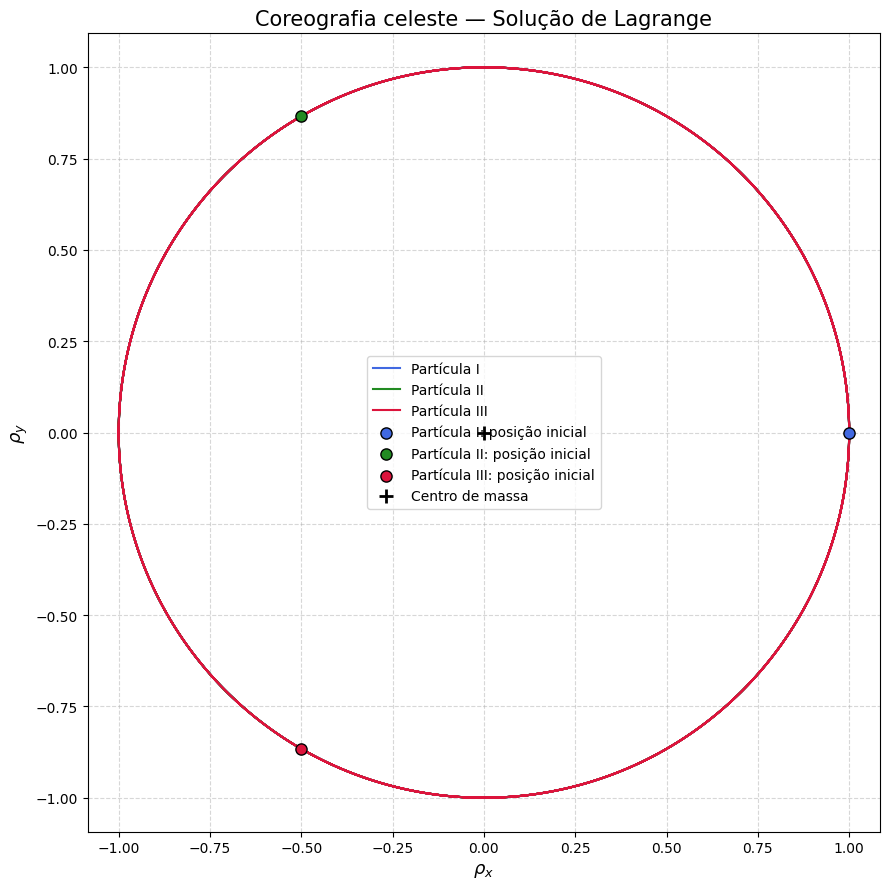
\includegraphics[width=0.9\textwidth]
    {tarefa-4a-grafico-1.png}
    \caption{Trajetórias das três partículas na solução de Lagrange para o problema gravitacional de três corpos.}
    \label{fig:coreografia-lagrange}
\end{figure}

Observa-se que as três trajetórias permanecem praticamente sobrepostas, formando uma circunferência de raio unitário em torno da origem. O gráfico também apresenta o centro de massa na origem, em concordância com as condições iniciais simétricas e com a igualdade das massas.

\subsection{Item (b): Solução periódica em forma de oito}

\subsubsection{Descrição do Problema}

Neste item, devem-se utilizar as condições iniciais fornecidas no enunciado para simular o movimento de três partículas de massas iguais, que apresentam uma configuração orbital periódica conhecida como ``O Oito''.

O objetivo é construir o gráfico das trajetórias das três partículas e apresentar suas posições em determinados instantes de tempo, de modo a acompanhar a evolução temporal da configuração. Essa solução foi descoberta por C. Moore em 1993.

% ORIENTAÇÕES À IA — ESTRATÉGIA DE SOLUÇÃO
% Consulte o código F77 e transcreva com cuidado as condições iniciais efetivamente utilizadas para as três partículas, incluindo massas, posições e velocidades.
% Apresente as equações gravitacionais de três corpos e explique a integração numérica implementada, incluindo o cálculo de todas as acelerações e a atualização temporal.
% Descreva como as trajetórias são armazenadas e como são selecionados os instantes de tempo mostrados para acompanhar a configuração. Informe passo temporal, duração e unidades.
% Se houver cálculo do período ou teste de retorno à condição inicial, explique o critério; caso contrário, limite a descrição à visualização das trajetórias e posições amostradas.
```latex
\subsubsection{Estratégia de Solução}

A única diferença deste código para o anterior é a declaração das condições iniciais.

\paragraph{Condições iniciais}

As posições e velocidades iniciais são escolhidas conforme a solução periódica em forma de oito:

\begin{equation}
    \vec{\rho}_{I,0}=
    (0,97000436,-0,24308753),
\end{equation}

\begin{equation}
    \vec{\upsilon}_{I,0}=
    (0,466203685,0,43236573),
\end{equation}

\begin{equation}
    \vec{\rho}_{II,0}=
    (-0,97000436,0,24308753),
\end{equation}

\begin{equation}
    \vec{\upsilon}_{II,0}=
    (0,466203685,0,43236573),
\end{equation}

\begin{equation}
    \vec{\rho}_{III,0}=(0,0),
\end{equation}

\begin{equation}
    \vec{\upsilon}_{III,0}=
    (-0,93240737,-0,86473146).
\end{equation}

\begin{lstlisting}[
style=fortranstyle
]
      program tarefa4b
      ! Coreografia celeste: figure-eight choreography com método Runge-Kutta de 4a ordem.
      ! Retorna ρ(τ) de três partículas gravitando em forma de 8
      ! Utiliza-se a 3a Lei de Kepler GM = 4pi^2 UA^3 ano^(-2).
      ! Grandezas adimensionais rho = r/UA, tau = 2pi*t/ano, v = v/(2pi*UA/ano).

      implicit none

      character(30) filename
      real*8 taumax, dtau
      real*8 mu_i, mu_ii, mu_iii
      real*8 rx_i(200000), ry_i(200000), vx_i, vy_i
      real*8 rx_ii(200000), ry_ii(200000), vx_ii, vy_ii
      real*8 rx_iii(200000), ry_iii(200000), vx_iii, vy_iii
      real*8 pi
      parameter (pi = 3.14159265358979323d0)

      ! Massas das partículas (adimensionais com o Sol)
      mu_i = 1.0d0
      mu_ii = 1.0d0
      mu_iii = 1.0d0

      ! Condições iniciais adimensionais
      ! Partícula I
      rx_i(1) = 0.97000436d0
      ry_i(1) = -0.24308753d0
      vx_i = 0.466203685d0
      vy_i = 0.43236573d0

      ! Partícula II
      rx_ii(1) = -0.97000436d0
      ry_ii(1) = 0.24308753d0
      vx_ii = 0.466203685d0
      vy_ii = 0.43236573d0

      ! Partícula III
      rx_iii(1) = 0.0d0
      ry_iii(1) = 0.0d0
      vx_iii = -0.93240737d0
      vy_iii = -0.86473146d0

      ! Parâmetros da simulação
      taumax = 5.0d0 * 2.0d0 * pi ! 5 anos de simulação
      dtau = 0.001d0 ! passo de tempo adimensional

      ! Nome do arquivo de saída
      filename = 'tarefa-4b-saida-1.dat'

      ! Chamada da subrotina de simulação
      call simulacao_orbita(
     &   filename,
     &   rx_i, ry_i, vx_i, vy_i,
     &   rx_ii, ry_ii, vx_ii, vy_ii,
     &   rx_iii, ry_iii, vx_iii, vy_iii,
     &   mu_i, mu_ii, mu_iii, dtau, taumax)

      end program


      subroutine simulacao_orbita(
     &   filename,
     &   rx_i, ry_i, vx_i, vy_i,
     &   rx_ii, ry_ii, vx_ii, vy_ii,
     &   rx_iii, ry_iii, vx_iii, vy_iii,
     &   mu_i, mu_ii, mu_iii, dtau, taumax)
      ! Simulacao via metodo de Runge-Kutta de quarta ordem
      ! Considera apenas a interacao gravitacional entre as tres particulas
      ! Retorna tau, rx, ry das particulas em um arquivo de saida
      implicit none
      character(30) filename

      real*8 rx_i(200000), ry_i(200000), vx_i, vy_i
      real*8 rx_ii(200000), ry_ii(200000), vx_ii, vy_ii
      real*8 rx_iii(200000), ry_iii(200000), vx_iii, vy_iii

      real*8 mu_i, mu_ii, mu_iii
      real*8 tau, dtau, taumax
      real*8 y(12), yt(12)
      real*8 k1(12), k2(12), k3(12), k4(12)
      integer*4 i, j, nsteps

      ! Numero de passos da simulacao
      nsteps = nint(taumax/dtau)

      ! Vetor de estado inicial
      y(1) = rx_i(1)
      y(2) = ry_i(1)
      y(3) = vx_i
      y(4) = vy_i

      y(5) = rx_ii(1)
      y(6) = ry_ii(1)
      y(7) = vx_ii
      y(8) = vy_ii

      y(9) = rx_iii(1)
      y(10) = ry_iii(1)
      y(11) = vx_iii
      y(12) = vy_iii

      ! Arquivo de saida
      open(10, file=filename, status='replace')

      write(10,*) 0.0d0,
     &   y(1), y(2), y(5), y(6), y(9), y(10)

      ! Integracao pelo metodo de Runge-Kutta de quarta ordem
      do i = 1, nsteps

        ! Primeiro estagio
        call derivadas(y, mu_i, mu_ii, mu_iii, k1)

        ! Segundo estagio
        do j = 1, 12
          yt(j) = y(j) + 0.5d0*dtau*k1(j)
        end do

        call derivadas(yt, mu_i, mu_ii, mu_iii, k2)

        ! Terceiro estagio
        do j = 1, 12
          yt(j) = y(j) + 0.5d0*dtau*k2(j)
        end do

        call derivadas(yt, mu_i, mu_ii, mu_iii, k3)

        ! Quarto estagio
        do j = 1, 12
          yt(j) = y(j) + dtau*k3(j)
        end do

        call derivadas(yt, mu_i, mu_ii, mu_iii, k4)

        ! Atualizacao do vetor de estado
        do j = 1, 12
          y(j) = y(j) + (dtau/6.0d0)*
     &       (k1(j) + 2.0d0*k2(j)
     &       + 2.0d0*k3(j) + k4(j))
        end do

        ! Armazenamento das posicoes
        rx_i(i+1) = y(1)
        ry_i(i+1) = y(2)

        rx_ii(i+1) = y(5)
        ry_ii(i+1) = y(6)

        rx_iii(i+1) = y(9)
        ry_iii(i+1) = y(10)

        ! Escrita no arquivo de saida
        tau = dble(i)*dtau

        write(10,*) tau,
     &       rx_i(i+1), ry_i(i+1),
     &       rx_ii(i+1), ry_ii(i+1),
     &       rx_iii(i+1), ry_iii(i+1)

      end do

      close(10)
      end subroutine

      
      subroutine derivadas(y, mu_i, mu_ii, mu_iii, dydtau)
      ! Calcula as derivadas do vetor de estado
      ! Sistema gravitacional de tres particulas
      implicit none

      real*8 y(12), dydtau(12)
      real*8 mu_i, mu_ii, mu_iii
      real*8 aceleracao

      ! Particula I
      dydtau(1) = y(3)
      dydtau(2) = y(4)

      dydtau(3) = mu_ii*aceleracao('x',
     &   y(1), y(2), y(5), y(6))
     &   + mu_iii*aceleracao('x',
     &   y(1), y(2), y(9), y(10))

      dydtau(4) = mu_ii*aceleracao('y',
     &   y(1), y(2), y(5), y(6))
     &   + mu_iii*aceleracao('y',
     &   y(1), y(2), y(9), y(10))

      ! Particula II
      dydtau(5) = y(7)
      dydtau(6) = y(8)

      dydtau(7) = mu_i*aceleracao('x',
     &   y(5), y(6), y(1), y(2))
     &   + mu_iii*aceleracao('x',
     &   y(5), y(6), y(9), y(10))

      dydtau(8) = mu_i*aceleracao('y',
     &   y(5), y(6), y(1), y(2))
     &   + mu_iii*aceleracao('y',
     &   y(5), y(6), y(9), y(10))

      ! Particula III
      dydtau(9) = y(11)
      dydtau(10) = y(12)

      dydtau(11) = mu_i*aceleracao('x',
     &   y(9), y(10), y(1), y(2))
     &   + mu_ii*aceleracao('x',
     &   y(9), y(10), y(5), y(6))

      dydtau(12) = mu_i*aceleracao('y',
     &   y(9), y(10), y(1), y(2))
     &   + mu_ii*aceleracao('y',
     &   y(9), y(10), y(5), y(6))

      return
      end subroutine


      function aceleracao(
     &   componente, rx_corpo_1, ry_corpo_1, rx_corpo_2, ry_corpo_2)
      ! Calcula a aceleração de um corpo devido à gravidade de outro corpo
      ! componente: 'x' para x, 'y' para y
      ! rx_corpo_1, ry_corpo_1: posição do corpo que sofre a aceleração
      ! rx_corpo_2, ry_corpo_2: posição do corpo que exerce a força gravitacional
      implicit none
      character*1 componente
      real*8 rx_corpo_1, ry_corpo_1, rx_corpo_2, ry_corpo_2
      real*8 aceleracao, r
      r = sqrt((rx_corpo_2 - rx_corpo_1)**2 + 
     & (ry_corpo_2 - ry_corpo_1)**2)
      if (componente .eq. 'x') then
        aceleracao = - (rx_corpo_1 - rx_corpo_2) / r**3
      else if (componente .eq. 'y') then
        aceleracao = - (ry_corpo_1 - ry_corpo_2) / r**3
      end if
      return
      end function
\end{lstlisting}


% ORIENTAÇÕES À IA — RESULTADOS OBTIDOS
% Apresente o gráfico das trajetórias das três partículas e as posições nos instantes efetivamente selecionados, com legenda e escala adequadas.
% Interprete a configuração em forma de oito, descrevendo a relação entre os movimentos das partículas e a evolução temporal observada.
% Avalie a periodicidade apenas na medida sustentada pelos dados: quantifique o retorno ao estado inicial ou ao padrão orbital se isso tiver sido calculado; caso contrário, descreva a recorrência visual sem afirmar periodicidade exata.
% Comente eventuais diferenças numéricas entre a trajetória obtida e a configuração ideal, se observáveis.
\subsubsection{Resultados Obtidos}

A Figura \ref{fig:coreografia-oito} apresenta as trajetórias das três partículas durante os cinco anos de integração numérica.

\begin{figure}[htbp]
    \centering
    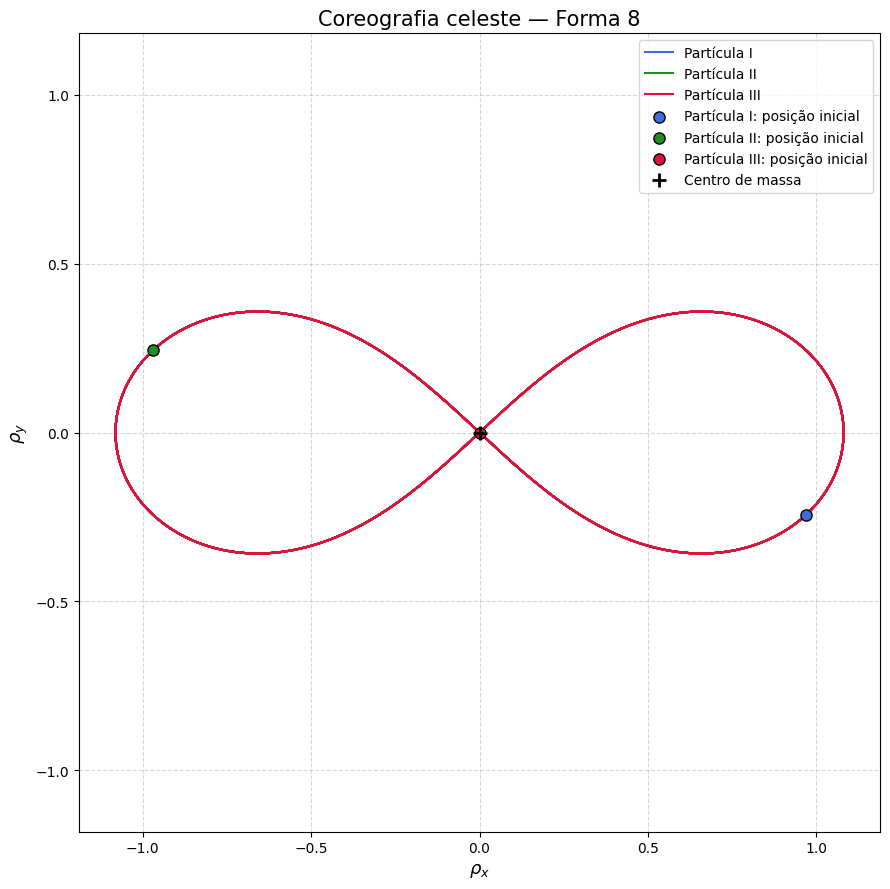
\includegraphics[width=0.9\textwidth]
    {tarefa-4b-grafico-1.png}
    \caption{Trajetórias das três partículas na solução periódica em forma de oito.}
    \label{fig:coreografia-oito}
\end{figure}

Observa-se que as três partículas percorrem trajetórias praticamente sobrepostas, formando uma curva em formato de oito. Diferentemente da solução de Lagrange apresentada no item anterior, não são descritas circunferências independentes: as três partículas percorrem uma mesma curva, em diferentes fases do movimento.

O centro de massa permanece na origem, conforme esperado a partir das condições iniciais simétricas e da conservação do momento linear total.

\subsection{Item (c): Perturbação da solução em forma de oito}

\subsubsection{Descrição do Problema}

Neste item, deve-se investigar a estabilidade da solução periódica em forma de oito, modificando-se a coordenada inicial $\rho_{x,0}$ da partícula 1, originalmente igual a $0{,}97000436$, para $0{,}95000436$.

O objetivo é observar como essa pequena alteração na condição inicial modifica a evolução temporal do sistema e verificar o que acontece com a configuração orbital em forma de oito.

% ORIENTAÇÕES À IA — ESTRATÉGIA DE SOLUÇÃO
% Leia o código F77 e identifique precisamente a alteração da coordenada inicial ρ_x,0 da partícula 1, de 0,97000436 para 0,95000436.
\subsubsection{Estratégia de Solução}

Neste item, investiga-se a sensibilidade da solução em forma de oito a pequenas perturbações nas condições iniciais. Para isso, mantém-se a configuração do item anterior, modificando exclusivamente a coordenada inicial $\rho_{x,0}$ da partícula I:

\begin{equation}
    \rho_{I,x}(0)=0,95000436,
\end{equation}

em substituição ao valor original $0,97000436$. Portanto, a perturbação introduzida corresponde a

\begin{equation}
    \Delta\rho_{I,x}=-0,02.
\end{equation}

As demais condições iniciais permanecem inalteradas, assim como as massas das partículas, que continuam sendo unitárias. As equações gravitacionais e o procedimento de integração também são os mesmos do item anterior.

As posições das três partículas são armazenadas no arquivo \texttt{tarefa-4c-saida-1.dat}, permitindo representar suas trajetórias e acompanhar a alteração da configuração orbital ao longo do tempo.

\begin{lstlisting}[
style=fortranstyle
]
      program tarefa4c
      ! Coreografia celeste: figure-eight choreography perturbada com método Runge-Kutta de 4a ordem.
      ! Retorna ρ(τ) de três partículas gravitando em forma de 8 até precessionar
      ! Utiliza-se a 3a Lei de Kepler GM = 4pi^2 UA^3 ano^(-2).
      ! Grandezas adimensionais rho = r/UA, tau = 2pi*t/ano, v = v/(2pi*UA/ano).

      implicit none

      character(30) filename
      real*8 taumax, dtau
      real*8 mu_i, mu_ii, mu_iii
      real*8 rx_i(200000), ry_i(200000), vx_i, vy_i
      real*8 rx_ii(200000), ry_ii(200000), vx_ii, vy_ii
      real*8 rx_iii(200000), ry_iii(200000), vx_iii, vy_iii
      real*8 pi
      parameter (pi = 3.14159265358979323d0)

      ! Massas das partículas (adimensionais com o Sol)
      mu_i = 1.0d0
      mu_ii = 1.0d0
      mu_iii = 1.0d0

      ! Condições iniciais adimensionais
      ! A única diferença em relação à tarefa4b é que a posição inicial da Partícula I foi perturbada em 0.02 UA no eixo x.
      ! Partícula I
      rx_i(1) = 0.95000436d0 ! perturbada
      ry_i(1) = -0.24308753d0
      vx_i = 0.466203685d0
      vy_i = 0.43236573d0

      ! Partícula II
      rx_ii(1) = -0.97000436d0
      ry_ii(1) = 0.24308753d0
      vx_ii = 0.466203685d0
      vy_ii = 0.43236573d0

      ! Partícula III
      rx_iii(1) = 0.0d0
      ry_iii(1) = 0.0d0
      vx_iii = -0.93240737d0
      vy_iii = -0.86473146d0

      ! Parâmetros da simulação
      taumax = 5.0d0 * 2.0d0 * pi ! 5 anos de simulação
      dtau = 0.001d0 ! passo de tempo adimensional

      ! Nome do arquivo de saída
      filename = 'tarefa-4c-saida-1.dat'

      ! Chamada da subrotina de simulação
      call simulacao_orbita(
     &   filename,
     &   rx_i, ry_i, vx_i, vy_i,
     &   rx_ii, ry_ii, vx_ii, vy_ii,
     &   rx_iii, ry_iii, vx_iii, vy_iii,
     &   mu_i, mu_ii, mu_iii, dtau, taumax)

      end program


      subroutine simulacao_orbita(
     &   filename,
     &   rx_i, ry_i, vx_i, vy_i,
     &   rx_ii, ry_ii, vx_ii, vy_ii,
     &   rx_iii, ry_iii, vx_iii, vy_iii,
     &   mu_i, mu_ii, mu_iii, dtau, taumax)
      ! Simulacao via metodo de Runge-Kutta de quarta ordem
      ! Considera apenas a interacao gravitacional entre as tres particulas
      ! Retorna tau, rx, ry das particulas em um arquivo de saida
      implicit none
      character(30) filename

      real*8 rx_i(200000), ry_i(200000), vx_i, vy_i
      real*8 rx_ii(200000), ry_ii(200000), vx_ii, vy_ii
      real*8 rx_iii(200000), ry_iii(200000), vx_iii, vy_iii

      real*8 mu_i, mu_ii, mu_iii
      real*8 tau, dtau, taumax
      real*8 y(12), yt(12)
      real*8 k1(12), k2(12), k3(12), k4(12)
      integer*4 i, j, nsteps

      ! Numero de passos da simulacao
      nsteps = nint(taumax/dtau)

      ! Vetor de estado inicial
      y(1) = rx_i(1)
      y(2) = ry_i(1)
      y(3) = vx_i
      y(4) = vy_i

      y(5) = rx_ii(1)
      y(6) = ry_ii(1)
      y(7) = vx_ii
      y(8) = vy_ii

      y(9) = rx_iii(1)
      y(10) = ry_iii(1)
      y(11) = vx_iii
      y(12) = vy_iii

      ! Arquivo de saida
      open(10, file=filename, status='replace')

      write(10,*) 0.0d0,
     &   y(1), y(2), y(5), y(6), y(9), y(10)

      ! Integracao pelo metodo de Runge-Kutta de quarta ordem
      do i = 1, nsteps

        ! Primeiro estagio
        call derivadas(y, mu_i, mu_ii, mu_iii, k1)

        ! Segundo estagio
        do j = 1, 12
          yt(j) = y(j) + 0.5d0*dtau*k1(j)
        end do

        call derivadas(yt, mu_i, mu_ii, mu_iii, k2)

        ! Terceiro estagio
        do j = 1, 12
          yt(j) = y(j) + 0.5d0*dtau*k2(j)
        end do

        call derivadas(yt, mu_i, mu_ii, mu_iii, k3)

        ! Quarto estagio
        do j = 1, 12
          yt(j) = y(j) + dtau*k3(j)
        end do

        call derivadas(yt, mu_i, mu_ii, mu_iii, k4)

        ! Atualizacao do vetor de estado
        do j = 1, 12
          y(j) = y(j) + (dtau/6.0d0)*
     &       (k1(j) + 2.0d0*k2(j)
     &       + 2.0d0*k3(j) + k4(j))
        end do

        ! Armazenamento das posicoes
        rx_i(i+1) = y(1)
        ry_i(i+1) = y(2)

        rx_ii(i+1) = y(5)
        ry_ii(i+1) = y(6)

        rx_iii(i+1) = y(9)
        ry_iii(i+1) = y(10)

        ! Escrita no arquivo de saida
        tau = dble(i)*dtau

        write(10,*) tau,
     &       rx_i(i+1), ry_i(i+1),
     &       rx_ii(i+1), ry_ii(i+1),
     &       rx_iii(i+1), ry_iii(i+1)

      end do

      close(10)
      end subroutine

      
      subroutine derivadas(y, mu_i, mu_ii, mu_iii, dydtau)
      ! Calcula as derivadas do vetor de estado
      ! Sistema gravitacional de tres particulas
      implicit none

      real*8 y(12), dydtau(12)
      real*8 mu_i, mu_ii, mu_iii
      real*8 aceleracao

      ! Particula I
      dydtau(1) = y(3)
      dydtau(2) = y(4)

      dydtau(3) = mu_ii*aceleracao('x',
     &   y(1), y(2), y(5), y(6))
     &   + mu_iii*aceleracao('x',
     &   y(1), y(2), y(9), y(10))

      dydtau(4) = mu_ii*aceleracao('y',
     &   y(1), y(2), y(5), y(6))
     &   + mu_iii*aceleracao('y',
     &   y(1), y(2), y(9), y(10))

      ! Particula II
      dydtau(5) = y(7)
      dydtau(6) = y(8)

      dydtau(7) = mu_i*aceleracao('x',
     &   y(5), y(6), y(1), y(2))
     &   + mu_iii*aceleracao('x',
     &   y(5), y(6), y(9), y(10))

      dydtau(8) = mu_i*aceleracao('y',
     &   y(5), y(6), y(1), y(2))
     &   + mu_iii*aceleracao('y',
     &   y(5), y(6), y(9), y(10))

      ! Particula III
      dydtau(9) = y(11)
      dydtau(10) = y(12)

      dydtau(11) = mu_i*aceleracao('x',
     &   y(9), y(10), y(1), y(2))
     &   + mu_ii*aceleracao('x',
     &   y(9), y(10), y(5), y(6))

      dydtau(12) = mu_i*aceleracao('y',
     &   y(9), y(10), y(1), y(2))
     &   + mu_ii*aceleracao('y',
     &   y(9), y(10), y(5), y(6))

      return
      end subroutine


      function aceleracao(
     &   componente, rx_corpo_1, ry_corpo_1, rx_corpo_2, ry_corpo_2)
      ! Calcula a aceleração de um corpo devido à gravidade de outro corpo
      ! componente: 'x' para x, 'y' para y
      ! rx_corpo_1, ry_corpo_1: posição do corpo que sofre a aceleração
      ! rx_corpo_2, ry_corpo_2: posição do corpo que exerce a força gravitacional
      implicit none
      character*1 componente
      real*8 rx_corpo_1, ry_corpo_1, rx_corpo_2, ry_corpo_2
      real*8 aceleracao, r
      r = sqrt((rx_corpo_2 - rx_corpo_1)**2 + 
     & (ry_corpo_2 - ry_corpo_1)**2)
      if (componente .eq. 'x') then
        aceleracao = - (rx_corpo_1 - rx_corpo_2) / r**3
      else if (componente .eq. 'y') then
        aceleracao = - (ry_corpo_1 - ry_corpo_2) / r**3
      end if
      return
      end function
\end{lstlisting}


% ORIENTAÇÕES À IA — RESULTADOS OBTIDOS
% Apresente as trajetórias do caso perturbado e compare-as com a solução de referência em forma de oito, usando gráficos ou dados efetivamente fornecidos.
% Descreva quando e como a configuração se afasta do padrão em forma de oito. Quantifique a divergência temporal se houver dados comparáveis para os dois casos.
% Interprete o resultado como resposta a uma perturbação das condições iniciais. Não conclua, com base em uma única perturbação e em tempo finito, uma classificação rigorosa de estabilidade ou caos sem análise adicional.
% Discuta a influência potencial do passo temporal e de erros numéricos, distinguindo-os da amplificação física da perturbação.
\subsubsection{Resultados Obtidos}

A Figura \ref{fig:coreografia-oito-perturbada} apresenta as trajetórias das três partículas após a perturbação da condição inicial.

\begin{figure}[htbp]
    \centering
    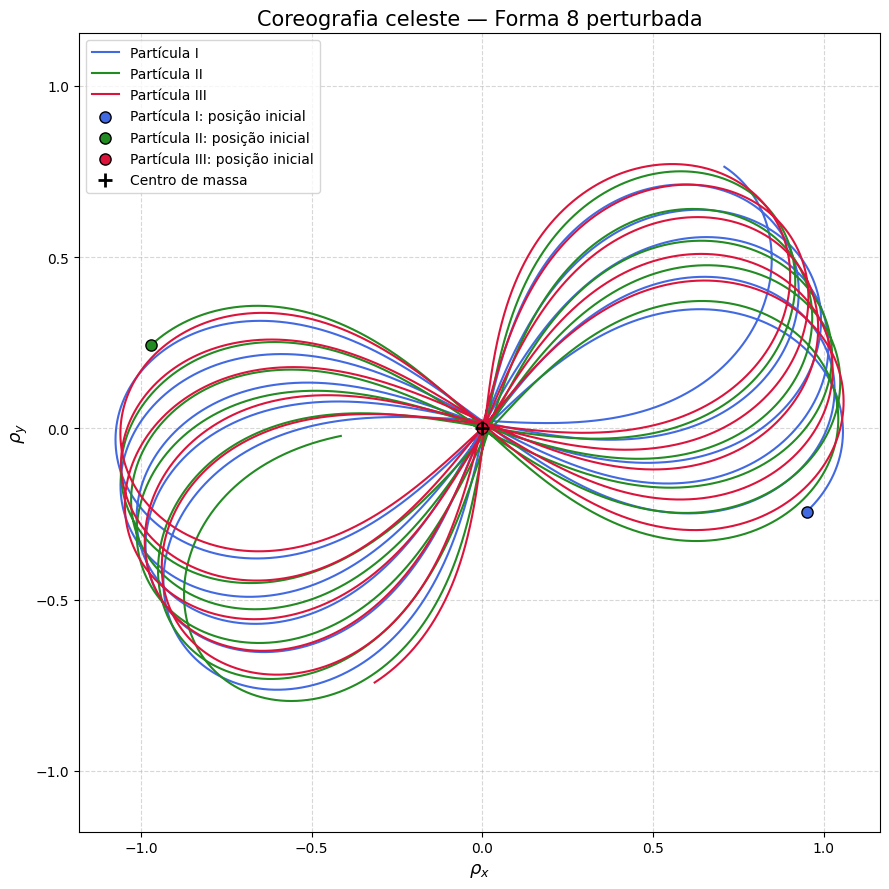
\includegraphics[width=0.9\textwidth]
    {tarefa-4c-grafico-1.png}
    \caption{Trajetórias das três partículas após a perturbação da condição inicial da partícula I.}
    \label{fig:coreografia-oito-perturbada}
\end{figure}

Observa-se que a configuração original em forma de oito deixa de ser preservada. A perturbação inicial é pequena, mas provoca alterações progressivas na evolução do sistema. Esse resultado evidencia a sensibilidade da coreografia às condições iniciais.

Além disso, a animação da simulação sugere uma aparente precessão da configuração em forma de oito: ao longo do tempo, a orientação da figura parece girar gradualmente em torno do centro de massa

\end{document}